% Digital Mohalla (F26-188) -- FYP-1 Mid-Evaluation Report, Iteration 1
% Built on the distributed FAST-NUCES template (fast-nuces-bs.cls, unmodified).
% Compile: pdflatex main -> bibtex main -> pdflatex main -> pdflatex main
\PassOptionsToPackage{obeyspaces,spaces}{url}
\documentclass[oneside]{fast-nuces-bs}
%\documentclass{article}

\usepackage{blindtext}
\usepackage{mathptmx}% Times Roman font
\usepackage[T1]{fontenc}
\usepackage{lipsum}
\usepackage{sectsty}
\usepackage{tikz-uml}
\usepackage{titlesec}
% Packages used by the chapter files (tables, figures, lists)
\usepackage{longtable}
\usepackage{booktabs}
\usepackage{array}
\usepackage{float}
\usepackage{enumitem}
\usepackage{xcolor}
\usetikzlibrary{shapes.geometric,arrows.meta}
% The class loads natbib with both "numbers" and "authoryear"; the references are
% numbered (IEEEtran), so select numeric citations in square brackets.
\setcitestyle{numbers,square,comma}

% Information about the Thesis
% -----------------------------------------------------------------------------
% (All are compulsory, do not delete any line other than author Information)
% For e.g., usually there are 3 students in a group, so leave authorone,
% authortwo, and authorthree, and delete authorfour.
%%%%%%%%%%%%%%%%%%%%%%%%%%%%%%%%%%%%%%%%%%%%%%%%%%%%%%%%%%%%%%%%%%%%%%%%%%%%%%%
\department{FAST School of Computing}
\faculty{Computer Science}
\degreeyear{2026}
\degreemonth{October}
\degreename{Computer Science}
\campuscity{Islamabad}
\authorone{Fatima Khursheed}{23i-0746}
\authortwo{Areeba Javed}{23i-0570}
\authorthree{Minahil Kashif}{23i-0554}
\supervisor{Dr. Ali Zeeshan}
\sessionduration{2023--2027}
% No co-supervisor for this project, so \cosupervisor is not set (template instruction).
\deanname{Dr. Dean Computing}
\directorname{Dr. Director of the Campus}
\hodname{Dr. Head of Computer Science Department}
\fypcoordinatorname{Name of FYP Coordinator}
\title{Digital Mohalla: A Trust-Based Platform for Neighbors}
%%%%%%%%%%%%%%%%%%%%%%%%%%%%%%%%%%%%%%%%%%%%%%%%%%%%%%%%%%%%%%%%%%%%%%%%%%%%%%%

% Names used by the front-matter chapters
\newcommand{\projecttitle}{Digital Mohalla: A Trust-Based Platform for Neighbors}
\newcommand{\projectid}{F26-188}
\newcommand{\studentone}{Fatima Khursheed (23i-0746)}
\newcommand{\studenttwo}{Areeba Javed (23i-0570)}
\newcommand{\studentthree}{Minahil Kashif (23i-0554)}

% Inline code, file names and identifiers (small typewriter; may break after / . _)
\DeclareUrlCommand\code{\def\UrlFont{\small\ttfamily}}
% Layout settings carried over from the V2 source
\setlist{itemsep=2pt,topsep=4pt}
\renewcommand{\arraystretch}{1.15}
\setcounter{tocdepth}{1}
% Long identifiers such as INSUFFICIENT_EVIDENCE may break after the underscore
\let\dmunderscore\_
\renewcommand{\_}{\dmunderscore\allowbreak}

% Tables: ragged-right paragraph columns
% Let TeX loosen a line slightly instead of letting long identifiers overflow
\setlength{\emergencystretch}{3em}

\newcolumntype{L}[1]{>{\raggedright\arraybackslash}p{#1}}
\newcolumntype{R}[1]{>{\raggedleft\arraybackslash}p{#1}}
\setlength{\LTpre}{0.5em}
\setlength{\LTpost}{0.5em}

% Diagrams too large to read on an A4 page: the picture plus a link that opens
% the full-size, zoomable diagram in draw.io (diagrams.net viewer).
% #1 = file name in figures/diagrams and figures/drawio_links,
% #2 = path of the source file in the design folder.
\newcommand{\drawionote}[2]{%
  \par\vspace{0.4em}{\small\centering
  Full-size diagram: \input{figures/drawio_links/#1}\\
  Source: \code{#2}\par}}

% Title page in the template's layout, with the report type and project ID
% added. The table of contents and the lists are printed after the front
% matter (see below), so the title page does not repeat them.
\makeatletter
\renewcommand{\maketitle}{%
\begin{alwayssingle}
    \thispagestyle{empty}
    \begin{center}
        { \setstretch{1}
        \par{\fontsize{24}{28}\selectfont \textbf{\@title}}\par
        \vspace{0.8cm}
        \par{\fontsize{14}{14}\selectfont FYP-1 Mid-Evaluation Report (Iteration 1)}\par
        \vspace{0.3cm}
        \par{\fontsize{14}{14}\selectfont Project ID: \projectid}\par
        \vspace{1cm}
        \par{\fontsize{14}{14}\selectfont Project Team}\\~\\
        {\fontsize{16}{16}\selectfont
        \begin{tabular}{lr}
            \@authoronename & \@authoroneroll \\
            \@authortwoname & \@authortworoll \\
            \@authorthreename & \@authorthreeroll
        \end{tabular}
        }\par
        \vspace{0.4cm}
        \par{\fontsize{14}{14}\selectfont Session \@sessionduration}\par
        \vspace{1.2cm}
        \par{\fontsize{14}{14}\selectfont Supervised by}\\~\\
        {\fontsize{17}{17}\selectfont \@supervisor}\par
        \vspace{.5cm}
        \begin{figure}[h]\centering
            
\includegraphics[width=.30\columnwidth]{ThesisFigs/FASTLogo}
        \end{figure}
        \vspace{0.5cm}
        \par{\fontsize{15}{15}\selectfont \textbf{\@department}}\par
        \vspace{0.5cm}
        \par{\fontsize{15}{18}\selectfont \textbf{National University of
        Computer and Emerging Sciences\\\@campuscity, Pakistan}}\par
        \vspace{0.5cm}
        \par{\fontsize{15}{15}\selectfont \textbf{\@degreemonth, \@degreeyear}}\par
    }
    \end{center}
    \null\vfill
    \clearpage
\end{alwayssingle}
}
\makeatother

%%%%%%%%%%%%%%%%%%%%%%%%%%%%%%%%%%%%%%%%%%%%%%%%%%%%%%%%%%%%%%%%%%%%%%%%%%%%%%
% Former document starts below this
\begin{document}

\cleardoublepage
\pagenumbering{roman}
\chapter*{Students' Submission}
\addcontentsline{toc}{chapter}{Students' Submission}
We certify that this report is submitted as the FYP-1 mid-report for the project titled \textit{\projecttitle} (project ID F26-188).

The report describes the work of Iteration~1: the Part~A design baseline and the Part~B implementation in three vertical slices (A: workflow skeleton, B: assurance core, C: human review loop), as it stands in the repository on 14 October 2026. Items that are deferred, provisional or not yet measured are stated as such where they appear.

\vspace{1cm}
\begin{tabular}{p{0.58\textwidth}p{0.36\textwidth}}
Student 1: \studentone & Signature: \rule{0.18\textwidth}{0.4pt}\\[1cm]
Student 2: \studenttwo & Signature: \rule{0.18\textwidth}{0.4pt}\\[1cm]
Student 3: \studentthree & Signature: \rule{0.18\textwidth}{0.4pt}
\end{tabular}

\chapter*{Anti-Plagiarism Statement}
\addcontentsline{toc}{chapter}{Anti-Plagiarism Statement}
The students certify that this report is their own work and that all sources used in preparing the report have been appropriately acknowledged and referenced.

Generative AI tools were used during the project: Claude Code for drafting code, tests and documents, and GitHub Copilot for an earlier report draft and automated pull-request review comments. Their use is declared per module in Section~\ref{sec:tool-use} and recorded entry by entry in the project's AI usage log (\code{docs/\allowbreak{}ai-usage-log.\allowbreak{}md}). Open-source libraries are listed with their versions and licences in Section~\ref{sec:dependencies}.

\chapter*{Authors' Declaration}
\addcontentsline{toc}{chapter}{Authors' Declaration}
We declare that the work documented in this report represents the work completed by the project team up to the FYP-1 mid-report stage. Contributions, tools, external components, and relevant sources are disclosed where applicable.

Each member owns the modules assigned in the Iteration 1 plan (Table~\ref{tab:work-division-iteration-1}) and has reviewed, tested and can explain the design, code and tests of those modules. All data used in development and testing is synthetic and is labelled as synthetic.

\chapter*{Abstract}
\addcontentsline{toc}{chapter}{Abstract}
Neighbourhood lending ends in a physical handover between people who often have little or no shared history, so a platform has to decide whether a loan is safe from evidence that is sparse, indirect and open to manipulation. Digital Mohalla is a neighbourhood resource-sharing platform built around that decision. Its core is an assurance engine that combines a recency-weighted Beta posterior over a borrower's verified loan outcomes, bounded $k$-hop evidence through the community's trust graph and interpretable manipulation signals, and returns one of four evidence states with its uncertainty, recommended safeguards and a written explanation; uncertain or suspicious cases go to a human moderator instead of being rejected automatically.

Iteration~1 delivered a live core: an event-sourced borrowing lifecycle (14 states; every lifecycle rule, namely allowed transitions, actor roles, no double booking and append-only events, is also enforced in PostgreSQL), the assurance engine, disputes and moderator decisions, a resident and moderator app, and a CI/CD pipeline deploying to a public instance. \NBackendTests{} backend and \NFrontendTests{} frontend tests pass. All seven evaluation scenarios required at mid-term return the expected state and explanation, and eleven of the thirteen scenarios reproduce their expected state end to end on synthetic data. Parameters remain hypotheses until the FYP-2 evaluation, which this report plans.

\chapter*{Acknowledgments}
\addcontentsline{toc}{chapter}{Acknowledgments}
We thank our supervisor, Dr. Ali Zeeshan, for guidance throughout the project, and the proposal defence panel, whose feedback on location and on the depth of the technical challenge shaped the direction of this iteration. We also thank the faculty of the FAST School of Computing and the maintainers of the open-source tools listed in Section~\ref{sec:dependencies}.

\chapter*{Executive Summary}
\addcontentsline{toc}{chapter}{Executive Summary}

\textbf{Problem.} Neighbours lend to one another, but a loan ends with an item handed to someone the lender may not know. Existing platforms either show one averaged rating, which hides how little evidence stands behind it, or show nothing at all. Neighbourhood evidence is sparse (most members have few loans), role-dependent (a good lender is not necessarily a good borrower), indirect (a borrower may be known to the lender's neighbours but not to the lender) and manipulable (a small group can rate itself up). Digital Mohalla treats the question \textit{``is there enough trustworthy evidence for this loan?''} as its complex computing problem.

\textbf{Response to the proposal defence.} The panel approved the proposal with minor modifications and made three points: show that location is a real issue, the platform has positive social potential, and the technical challenge looked limited. The third point changed the project most. The team narrowed the first iteration to the assurance engine and the transaction lifecycle that feeds it, and answered the location point with a comparison of five locality methods, a threat model and eighteen test checks on the chosen rule (Chapter~\ref{ch:proposal-feedback-iteration}).

\textbf{What Iteration 1 delivered.} All three planned slices are complete and merged:
\begin{itemize}
\item \textbf{Slice A, workflow skeleton:} an append-only, hash-chained event store; a 14-state borrowing lifecycle whose transitions are checked in Python and again by a PostgreSQL foreign key; double booking prevented by a database exclusion constraint; login and a REST API; a resident app; CI and CD.
\item \textbf{Slice B, assurance core:} outcome extraction from closed loans, a recency-weighted Beta posterior with a 90\% credible interval and similarity weighting, trust edges and bounded $k$-hop search ($k=3$), a decision policy of rules R1--R9 (R6 in two variants) with safeguards and plain-language explanations, a scenario suite in CI and the lender's evidence screen.
\item \textbf{Slice C, human loop:} partner-clustering and review-similarity signals with a retaliation check, disputes that freeze a loan, moderator decisions on disputes and holds, privacy checks on every API response and log line, request fuzzing, and the moderator app.
\end{itemize}

\textbf{Evidence.} 623 backend tests (unit, integration on PostgreSQL 16, property-based and scenario tests) and 29 frontend tests pass in CI, with 97\% line coverage of the backend code, and every pull request runs them before merge. All seven scenarios required at mid-term (ES-01 to ES-06 and ES-13) return the documented state \textit{and} explanation, against a target of seven of thirteen (NFR-Q-01); eleven of the thirteen reproduce their expected state end to end on synthetic data. At $k=3$ the indirect-evidence search takes 4.5~ms at the 95th percentile on a 2,026-user synthetic graph and finds a path for 93.2\% of loan pairs. The API and the web app are deployed on Render with a Neon PostgreSQL database, from the \code{main} branch after CI passes.

\textbf{Honest limits.} All parameters (half-life, thresholds, decay, signal weights) are initial hypotheses checked only on synthetic data. The locality method is designed but not built; photo uploads, the audit-log screen, three manipulation signals (S2, S3, S5) and the scheduler move to Iteration 2. Generative AI (Claude Code) drafted most first-draft code under the team's direction; its use is declared per module in Section~\ref{sec:tools-tool-assisted-development}.

\textbf{Next.} Iteration 2 completes the core modules (membership and locality, the remaining lifecycle timers, the remaining signals and reviews, case information requests and appeals) and builds the simulator, baselines and FYP-2 evaluation plan that will test whether the engine's uncertainty actually improves decisions over simple averages.

\tableofcontents
\listoffigures
\listoftables
\chapter*{List of Abbreviations}
\addcontentsline{toc}{chapter}{List of Abbreviations}
\begin{longtable}{L{0.16\textwidth}L{0.76\textwidth}}
\toprule Abbreviation & Meaning \\ \midrule \endfirsthead
\toprule Abbreviation & Meaning \\ \midrule \endhead
ADR & Architecture Decision Record \\
API & Application Programming Interface \\
AWS & Amazon Web Services \\
CCP & Complex Computing Problem \\
CD & Continuous Deployment \\
CI & Continuous Integration \\
CI (in statistics) & Credible Interval \\
CNIC & Computerised National Identity Card \\
CORE / ENAB / SUPP / STRC & Requirement scope tags: core, core-enabling, supporting, stretch \\
D1--D20 & Team decisions recorded in \code{docs/\allowbreak{}design/\allowbreak{}00\_management/} \\
DEI & Diversity, Equity and Inclusion \\
DF & Defect (defect log entries DF-01 to DF-09) \\
DFD & Data Flow Diagram \\
ER, ERD & Entity--Relationship (Diagram) \\
ES & Evaluation Scenario (ES-01 to ES-13) \\
EXIF & Exchangeable Image File Format (photo metadata) \\
FK & Foreign Key \\
FR & Functional Requirement \\
FYP & Final Year Project \\
GPS & Global Positioning System \\
HCI & Human--Computer Interaction \\
HTTP(S) & Hypertext Transfer Protocol (Secure) \\
JSON & JavaScript Object Notation \\
JWT & JSON Web Token \\
L2, L3 & Levels of generative-AI use (assisted; core-assist), Section~\ref{sec:tool-use} \\
MoSCoW & Must, Should, Could, Won't (prioritisation) \\
NFR & Non-Functional Requirement \\
NUL & The null character (code 0) \\
P2P & Peer to Peer \\
P50, P95 & 50th and 95th percentile (latency) \\
PKR & Pakistani Rupee \\
PR & Pull Request; in NFR identifiers, Privacy \\
R1--R9 & Rules of the decision policy (Algorithm 4) \\
REST & Representational State Transfer \\
S1--S5 & Manipulation signals; in ownership tables, Students 1 to 3 \\
SDG & Sustainable Development Goal \\
SDK & Software Development Kit \\
SQL & Structured Query Language \\
SSD & System Sequence Diagram \\
SUS & System Usability Scale \\
TC & Test Case (Test Plan v1.3) \\
TF-IDF & Term Frequency--Inverse Document Frequency \\
TLS & Transport Layer Security \\
UC & Use Case \\
UI & User Interface \\
UML & Unified Modeling Language \\
UTC & Coordinated Universal Time \\
W1--W7 & Wireframes of the core screens \\
\bottomrule
\end{longtable}


\cleardoublepage
\pagenumbering{arabic}
\chapter{Introduction and Project Vision}
\label{ch:intro}

\section{Project Overview}
Digital Mohalla (\emph{mohalla}: neighbourhood) is a neighbourhood borrowing and lending platform. A member lists an item, a neighbour requests it for some dates, the lender decides, the item changes hands, and it comes back. Every step is recorded, and the outcome of each loan becomes evidence for the next one.

Its central computing problem is to decide whether a proposed loan has enough trustworthy evidence when history is sparse, role-dependent and possibly manipulated, while protecting location privacy and sending uncertain cases to people. A recency-weighted Beta posterior, bounded indirect evidence and interpretable manipulation signals produce an explained \emph{assurance state}; the platform never labels a person or issues a single trust score. Everything else in the platform (listings, workflow, search, interface) exists to feed that decision or to act on it.

\section{Problem Statement}
\begin{quote}
Determine whether a proposed borrowing transaction has sufficient trustworthy evidence under sparse, role-dependent and potentially manipulated history, while protecting location privacy and escalating uncertain cases to humans.
\end{quote}
Four properties make this hard:
\begin{enumerate}
\item \textbf{Sparse evidence.} Most neighbours have a handful of loans, or none. A newcomer with no history is not a risky person, so ``no evidence'' must not be reported as ``bad evidence''.
\item \textbf{Role dependence.} Returning items on time as a borrower says little about describing items honestly as a lender, so evidence is kept per role and metric.
\item \textbf{Indirect evidence.} A borrower may have a good record with the lender's neighbours but none with the lender. That evidence is useful but weaker than direct history and must never be enough on its own.
\item \textbf{Manipulation.} A small ring of accounts can rate one another up, and a lender can post a retaliatory review after a dispute. A real family that lends within itself looks statistically similar to such a ring, so signals must be evidence for a human, never an automatic verdict.
\end{enumerate}

\section{Problem Context and Motivation}
Lending between neighbours is an old practice; what a platform has to add is a way to make a handover between near-strangers feel safe. In the team's own experience of Pakistani neighbourhoods, such lending is arranged informally, in messaging groups and by word of mouth, which leaves no record of who borrowed what, no evidence of the item's condition and no process for resolving a dispute. Research on online marketplaces shows that the trust cues a platform chooses change behaviour \cite{ert2016trust} and that averaged reputation hides uncertainty and is easy to game \cite{josang2007survey}. The project therefore puts its effort into the quality of the evidence behind a decision, not into another listings app.

\section{Project Vision}
A neighbourhood platform where any member can lend to any other member with a clear, honest picture of the evidence behind the request: how much verified history exists, how certain it is, what the community knows, whether anything looks anomalous, and which safeguards are sensible. The platform supports the lender's decision and never makes it for them; whenever the evidence is uncertain or suspicious, a human moderator decides.

\section{Project Objectives}
\begin{enumerate}
\item Record every borrowing transaction as an immutable, replayable event stream in which invalid transitions and double bookings are impossible (NFR-R-01 to R-03: 100\% of runs).
\item Return, for every request, exactly one of four assurance states with its uncertainty, evidence, safeguards and explanation (FR-T-01), with direct-evidence assessment under 1~s at the 95th percentile (NFR-P-03).
\item Show that the engine behaves as designed on the evaluation scenarios: at least 7 of 13 at mid-term and 13 of 13 at the end, state and explanation both correct (NFR-Q-01).
\item Route every hold and dispute to a moderator, never restrict anyone automatically, and record each decision with a reason in a tamper-evident log (FR-T-11, FR-M-05).
\item Keep exact location and identity numbers out of every API response and log (NFR-PR-01, NFR-S-07).
\item In FYP-2, show that the full engine beats global-average and role-average baselines on Brier score and calibration, with each component justified by ablation (NFR-Q-02).
\end{enumerate}

\section{Project Scope}
The committed core is: community membership with privacy-preserving locality verification, borrowing requests, the event-sourced transaction lifecycle, evidence-based assurance, handover and return confirmation, dispute management and moderator review. Requirements are tagged CORE (named in the committed core), ENAB (core-enabling), SUPP (supporting) and STRC (stretch, only after the core works).

\textbf{Excluded} (or stretch only): vendors, community events, kameti (rotating savings), a general chatbot, a social feed, advertisements and broad analytics. Search and matching are supporting scope for Iteration~3. The project must not become a generic social network, a conventional listings app, a surveillance system, an opaque social-scoring system, or a large-language-model substitute for a computing challenge.

\section{Project Modules}
\label{sec:modules}
The platform is organised into the ten modules of the project overview. Table~\ref{tab:modules} gives each module's scope and its state after Iteration~1.

\begin{longtable}{L{0.04\textwidth}L{0.27\textwidth}L{0.13\textwidth}L{0.44\textwidth}}
\caption{The ten modules and their state after Iteration~1}\label{tab:modules}\\
\toprule
\# & Module & Scope & Iteration 1 \\ \midrule \endfirsthead
\toprule \# & Module & Scope & Iteration 1 \\ \midrule \endhead
1 & User \& Community Management & Core (membership, locality) & Password login and roles; communities, memberships and items seeded. Locality method designed (A11), build in Iteration~2 \\
2 & Community Events \& Activities & Stretch & Not started (by design) \\
3 & Resource Sharing \& Item Management & Core (lifecycle) & \textbf{Built}: event store, 14-state lifecycle, request, accept/decline/cancel, handover, return, disputes, replay, double-booking guard \\
4 & Search, Discovery \& Matching & Supporting & Not started; Iteration~3 \\
5 & Trust, Reputation \& Safety & \textbf{Core (CCP)} & \textbf{Built}: Beta posterior, similarity, trust edges, $k$-hop, two manipulation signals and the retaliation check, decision rules R1--R9 (R6 in two variants), explanations, engine-failure hold \\
6 & Community Forum \& Chatbot & Stretch & Not started (by design) \\
7 & Communication \& Notifications & Enabling & Not started; in-app notifications in Iteration~2 \\
8 & Vendor Management & Stretch & Not started (by design) \\
9 & Administration \& Moderation & Core (cases, disputes, audit) & \textbf{Built}: escalation cases with evidence trail, moderator decisions on disputes and holds, append-only hash-chained audit log; audit-log screen in Iteration~2 \\
10 & Analytics \& Reports & Core (event logging, evaluation) & \textbf{Built}: frozen event logging, synthetic dataset generator, scenario suite in CI, $k$ sweep \\
\bottomrule
\end{longtable}

\section{Stakeholders and User Classes}
\begin{longtable}{L{0.2\textwidth}L{0.72\textwidth}}
\caption{User classes}\label{tab:users}\\
\toprule User class & Characteristics and needs \\ \midrule \endfirsthead
\toprule User class & Characteristics and needs \\ \midrule \endhead
Borrower & Requests items for dates; needs a fair hearing even with no history; may raise or withdraw a dispute. \\
Lender & Owns items; decides requests from the evidence summary; records the handover checklist and deposit (record only, no money moves). \\
Newcomer & A borrower with no verified history; must receive INSUFFICIENT\_EVIDENCE with a route forward, never a negative label. \\
Moderator & A member trusted by one community; decides holds and disputes in that community only, always with a reason. \\
Admin & Manages communities, roles and categories (Iteration~2 onwards). \\
Community & The group of members who share a locality; the source of indirect evidence and the unit of moderation. \\
Project team and examiners & Need replayable events, versioned parameters and reproducible scenario results to evaluate the engine. \\
\bottomrule
\end{longtable}

\section{Success Criteria}
\begin{longtable}{L{0.3\textwidth}L{0.36\textwidth}L{0.26\textwidth}}
\caption{Measurable success criteria}\label{tab:success}\\
\toprule Criterion & Measure & Status after Iteration 1 \\ \midrule \endfirsthead
\toprule Criterion & Measure & Status after Iteration 1 \\ \midrule \endhead
No double booking (NFR-R-01) & Exactly one of N simultaneous acceptances commits, every run & Met (TC-08: 5 simultaneous acceptances, 3 rounds) \\
Invalid transitions rejected (NFR-R-02) & 100\% of invalid (state, event) pairs refused & Met (TC-01: all 294 state--event pairs, 263 refused) \\
Replay (NFR-R-03) & Rebuilt state equals stored state & Met (TC-07 and the replay tests of suite 2) \\
Tamper evidence (NFR-S-05) & 100\% of altered events detected & Met (TC-13, TC-14) \\
Configuration versioned (NFR-D-01) & 100\% of assessments store \code{config\_version} & Met (TC-71, database NOT NULL) \\
Scenario quality (NFR-Q-01) & $\geq$7 of 13 at mid-term, 13 of 13 final & 7 of 7 required pass; 11 of 13 states end to end \\
Assessment latency (NFR-P-03) & Direct evidence P95 $\leq$ 1~s & Not yet measured (Iteration~2); $k$-hop component only: P95 4.5~ms at $k=3$ \\
Privacy (NFR-PR-01, S-07) & No location or CNIC in any response or log & Met for the built API (suite 14) \\
Decision quality (NFR-Q-02) & Beats averaging baselines on Brier score and calibration & FYP-2 evaluation \\
Newcomer fairness (NFR-Q-07) & Assurance for new vs.\ established users reported & FYP-2 evaluation \\
\bottomrule
\end{longtable}

\section{Constraints and Assumptions}
\begin{itemize}
\item Three students and two semesters: no framework or abstraction is added unless a requirement needs it.
\item No real user data in FYP-1. All development and test data is synthetic, generated with a fixed seed and labelled synthetic in every file and screen. Public trust networks (Epinions, Bitcoin OTC) are used only for aggregate shape statistics; no rows are copied.
\item The team does not run interviews or surveys; the location question is answered by a method comparison, threat model and test cases (Section~\ref{sec:actions}).
\item Free-tier hosting (Render and Neon); the API sleeps when idle, so the first request after a pause is slow.
\item Every tunable parameter is an initial hypothesis kept in a versioned configuration file (currently \code{\ConfigVersion}) and is to be justified by the FYP-2 sensitivity analysis.
\item Android and web are the target clients; iOS is not targeted (team decision, 13 October).
\end{itemize}

\section{Ethical, Legal and DEI Considerations}
\begin{itemize}
\item \textbf{Decision support, not judgement.} Assurance states describe the evidence for a transaction, not the person. No screen shows a single trust number (NFR-U-01), and every state is shown with the evidence behind it.
\item \textbf{No automatic restriction.} Manipulation signals are anomalies with evidence, worded neutrally; a request is only ever held for a moderator, who must give a reason. Nothing is restricted without a human decision.
\item \textbf{Newcomers are not penalised.} Zero history yields INSUFFICIENT\_EVIDENCE with the message ``Insufficient verified history; lender review required'' and sensible safeguards, never a low score. Fairness between new and established users is a reported metric (NFR-Q-07).
\item \textbf{Privacy.} Only approximate (community-level) location is used; GPS is read once, in memory, when a member joins a community, and a borrowing request carries no location. No exact address or CNIC is stored. Automated tests check every API response model and log line.
\item \textbf{Consent.} Pilot data in FYP-2 will be collected with consent and a right to withdraw (NFR-PR-05); applicable Pakistani data-protection obligations are to be confirmed with the supervisor.
\item \textbf{Social value.} The project supports SDG~12 (responsible consumption, through reuse and local circulation) and SDG~11 (inclusive, safe communities).
\end{itemize}

\chapter{Research and Existing Solutions}\label{ch:research-existing-solutions}
\section{Research Method / Approach}\label{sec:research-method-approach}
The research had four strands, each feeding a specific design question:

\begin{enumerate}
\item \textbf{Literature on reputation and trust.} Beta reputation and its uncertainty \cite{josang2002beta,josang2016subjective}, surveys of trust and reputation systems \cite{josang2007survey,resnick2000}, trust propagation in social networks \cite{golbeck2005,kamvar2003}, graph anomaly and collusion detection \cite{akoglu2015,mukherjee2012,hooi2016}, and reciprocity in two-sided review systems \cite{bolton2013,fradkin2021}. Each source is cited where it shaped a decision, and the report states whether a method was reproduced, adapted or replaced.
\item \textbf{Products and prior projects.} The products residents use today and four earlier FAST final-year projects in the same space were compared on the features that matter for safe lending (Section~\ref{sec:comparison-existing-solutions}).
\item \textbf{Public data, for shape only.} Aggregate statistics of public trust networks (Epinions \cite{massa2007} and Bitcoin OTC/Alpha \cite{kumar2016,kumar2018}), such as degree distributions and the share of positive edges, were measured to make the synthetic neighbourhood data realistic. No rows from these datasets are copied into the project.
\item \textbf{Design-time verification.} Every algorithm was worked by hand on small examples (for instance an 8-node graph for the $k$-hop search and thirteen scenario fixtures for the decision policy) before code was written, and the code is tested against those worked numbers (Chapter~\ref{ch:testing-early-validation}).
\end{enumerate}

\section{Existing Solutions / Products}\label{sec:existing-solutions-products}
\begin{itemize}
\item \textbf{OLX and Facebook Marketplace} \cite{olx,fbmarketplace}. General classifieds. Strong reach and listings, but built for one-off sales between strangers; trust cues are a profile and, at most, a star average.
\item \textbf{WhatsApp groups and kameti apps.} In the team's experience, the informal channel through which neighbourhood lending is arranged today. Familiar and immediate, but there is no record of who borrowed what, no condition evidence and no dispute process. Kameti (rotating savings) apps digitise contributions \cite{mehmood2019} but not item lending.
\item \textbf{Nextdoor} \cite{nextdoor}. A neighbourhood social network with verified addresses and posts; lending is informal and outside any workflow.
\item \textbf{Peerby and Fat Llama} \cite{peerby,fatllama}. Peer-to-peer rental platforms with listings and booking flows; reputation is a review average, without a statement of how much evidence stands behind it.
\item \textbf{Prior FAST FYPs} (identified by their FAST FYP project IDs). Kiraya (F22-071) and AIRental (F23-029) address rentals, Kitabiyat (S25-040) book sharing and PawPal (F25-101) a pet community. None models evidence quality or manipulation.
\end{itemize}

\section{Comparison of Existing Solutions}\label{sec:comparison-existing-solutions}
Table~\ref{tab:comparison-existing-products-prior} repeats the comparison presented at the proposal defence. Ratings are the team's assessment of each product's public features at that time: $\checkmark$~supported, $\sim$~partial, $\times$ not supported.

\begin{table}[!htbp]
\centering
\caption{Comparison with existing products and prior projects (proposal defence)}\label{tab:comparison-existing-products-prior}
\resizebox{\textwidth}{!}{%
\begin{tabular}{@{}lccccccccc@{}}
\toprule
Feature & DM & OLX/FB & WA/kameti & Nextdoor & Peerby/FL & Kiraya & AIRental & Kitabiyat & PawPal \\
\midrule
P2P lending & $\checkmark$ & $\checkmark$ & $\sim$ & $\times$ & $\checkmark$ & $\sim$ & $\checkmark$ & $\checkmark$ & $\times$ \\
Shared reputation & $\checkmark$ & $\sim$ & $\times$ & $\sim$ & $\sim$ & $\times$ & $\times$ & $\times$ & $\sim$ \\
Trust-aware decisions & $\checkmark$ & $\times$ & $\times$ & $\times$ & $\sim$ & $\times$ & $\sim$ & $\sim$ & $\times$ \\
Moderation workflow & $\checkmark$ & $\sim$ & $\sim$ & $\sim$ & $\sim$ & $\times$ & $\times$ & $\times$ & $\sim$ \\
Unified neighbourhood platform & $\checkmark$ & $\times$ & $\times$ & $\checkmark$ & $\times$ & $\times$ & $\times$ & $\times$ & $\sim$ \\
\bottomrule
\end{tabular}}
\par\vspace{0.3em}{\footnotesize DM = Digital Mohalla; FB = Facebook; WA = WhatsApp; FL = Fat Llama. The DM column shows the proposal-time vision: ``Unified neighbourhood platform'' and ``Shared reputation'' describe the full platform. After the defence the scope was narrowed (Section~\ref{sec:project-modules}), and the engine reports evidence states for a loan rather than a reputation score for a person.\par}
\end{table}


After the defence the comparison was narrowed to the properties the assurance engine adds, which none of the compared products offers as a whole: (1) reporting how much verified evidence stands behind a judgement, with an interval, instead of an average; (2) keeping evidence per role; (3) using the community's indirect evidence while capping it below direct evidence; (4) treating manipulation as a separate risk dimension reviewed by a person; and (5) recording handover, return and disputes as evidence for future decisions.

\section{Limitations and Gaps}\label{sec:limitations-gaps}
\begin{itemize}
\item \textbf{Averages hide uncertainty.} A 5.0 from one review and a 4.8 from two hundred look alike, and averaged reputation is easy to game \cite{josang2007survey,resnick2000}.
\item \textbf{Newcomers are invisible or penalised.} Cold start cannot be solved by a model, because the history does not exist \cite{schein2002}; it needs an explicit policy.
\item \textbf{No evidence trail.} Informal channels record nothing about handover condition or returns, so a dispute is one person's word against another's.
\item \textbf{Manipulation is handled by deletion or not at all.} Where it is handled, it is usually an opaque automatic action, which is unacceptable in a neighbourhood where members cannot simply leave.
\end{itemize}

\section{Proposed Solution}\label{sec:proposed-solution}
Digital Mohalla records every loan as an immutable event stream and turns confirmed outcomes into evidence. For each request the assurance engine (i) estimates the borrower's reliability in the borrower role with a recency-weighted Beta posterior and a 90\% credible interval, (ii) adds capped indirect evidence from at most three hops in the lender's community, (iii) computes manipulation signals as a separate risk, and (iv) applies an ordered decision table that returns one of four states (SUFFICIENT\_EVIDENCE, REVIEW\_RECOMMENDED, INSUFFICIENT\_EVIDENCE, ACTIVE\_DISPUTE) with safeguards and an explanation. Requests the engine cannot clear are held for a moderator; nothing is rejected automatically.

\section{Complex Computing Problem}\label{sec:complex-computing-problem}
The problem meets the Seoul Accord characteristics of a complex computing problem (Table~\ref{tab:mapping-seoul-accord-complex}).

\begin{table}[!htbp]
\centering
\caption{Mapping to the Seoul Accord complex computing problem characteristics}\label{tab:mapping-seoul-accord-complex}
\begin{tabular}{@{}L{111pt}L{268pt}@{}}
\toprule
Characteristic & How Digital Mohalla meets it \\
\midrule
Depth of knowledge & Bayesian inference with recency weighting; bounded graph search with path-diversity rules; anomaly detection on review graphs and text; concurrency control and event sourcing in a relational database. \\
Conflicting requirements & Safety vs. inclusion of newcomers; manipulation detection vs. false suspicion of real families; trust verification vs. location privacy; explanation detail vs. disclosure of other members' data. \\
Depth of analysis, no obvious solution & No off-the-shelf model answers ``is there enough evidence for this loan''; the rule order, thresholds and caps had to be analysed on worked scenarios (ADR-0007, ADR-0008). \\
Infrequently encountered issues & Collusion in sparse graphs; retaliatory reviews after disputes; a ring that also trades with outsiders lowers its own density (camouflage \cite{hooi2016}). \\
Beyond standards and codes & Reputation averages, the usual practice, are what the design replaces. \\
Diverse stakeholders & Borrowers, lenders, newcomers, moderators, admins and the community as a whole, with different and sometimes opposed interests. \\
Significant consequences & A wrong ``sufficient'' risks a physical item and a relationship between neighbours; a wrong ``suspicious'' damages a person's standing in a place they cannot leave. \\
Interdependence & The engine depends on lifecycle evidence (only confirmed outcomes count), and the lifecycle depends on the engine (holds, safeguards); disputes feed back into evidence after a moderator rules. \\
Ill-defined requirements & ``Enough evidence'' has no external definition; thresholds are hypotheses to be calibrated in FYP-2 against baselines and ablations. \\
\bottomrule
\end{tabular}
\end{table}
\section{Technical Challenges}\label{sec:technical-challenges}
\begin{enumerate}
\item \textbf{Concurrent acceptances.} Two lenders' (or one lender's two) acceptances for overlapping dates can race. Solved in the database: an exclusion constraint on held bookings makes the second commit fail, and the transition, booking and event commit in one transaction (ADR-0002).
\item \textbf{Correctness of the lifecycle under every command.} 14 states and 21 event types give 294 pairs; only 31 are valid. The transition table is enforced in Python and by a composite foreign key in PostgreSQL, and all 294 pairs are tested.
\item \textbf{Uncertainty under sparse data.} The posterior must distinguish ``no evidence'' from ``bad evidence''; the effective evidence count $n_{\mathrm{eff}}$ and the interval's lower bound enter the rules directly.
\item \textbf{Correlated indirect evidence.} Several paths through the same neighbour are not independent; only the strongest path per first-hop neighbour is kept before combining with noisy-OR.
\item \textbf{Latency of graph search.} Path enumeration grows quickly with $k$; the $k=1$ to 4 sweep (Section~\ref{sec:algorithm-2-bounded-hop-indirect}) measured a 3.5-fold rise in 95th-percentile latency from $k=3$ to $k=4$ for one percentage point more coverage.
\item \textbf{Real families vs. rings.} A family that lends within itself fills its review graph like a ring. A hold now needs two corroborating signals (ADR-0007), so one strong signal alone only asks for verification.
\item \textbf{Engine failure.} A slow or failing engine must never yield a default state; requests are held with reason \code{engine_failure} after a 2,000 ms timeout.
\end{enumerate}

\section{Research Findings and Design Decisions}\label{sec:research-findings-design-decisions}
\begingroup
\begin{longtable}{@{}L{136pt}L{69pt}L{170pt}@{}}
\caption{How research findings shaped the design}\label{tab:how-research-findings-shaped}\\
\toprule
Finding & Source & Design consequence \\
\midrule
\endfirsthead
\toprule
Finding & Source & Design consequence \\
\midrule
\endhead
\bottomrule
\endlastfoot
Averaged reputation hides uncertainty and is easy to game & \cite{josang2007survey,resnick2000} & Report a posterior with a 90\% interval and effective evidence; never show a single number (NFR-U-01). \\
Binary outcomes have a conjugate Beta posterior & \cite{josang2002beta} & \textit{Adapted}: Beta(1,1) prior updated with outcomes weighted by a 180-day half-life, kept per role and metric. \\
Trust propagates with decreasing influence & \cite{golbeck2005} & \textit{Adapted}: bounded $k$-hop paths with decay $\gamma^{h-1}$, one path per first hop, noisy-OR, capped at $\rho \leq 0.6$. A global score such as EigenTrust \cite{kamvar2003} was not used, because it gives every user one number. \\
Two-sided reviews are reciprocal by nature & \cite{bolton2013,fradkin2021} & ``A rated B and B rated A'' was rejected as a signal; on the synthetic data it flagged 6 of 8 ordinary members (decision D18). \\
Collusion shows as groups that rate one another & \cite{mukherjee2012,hooi2016} & S1 measures how many of a member's review partners also reviewed each other both ways (partner clustering, D18). \\
Graph anomaly methods trade accuracy for interpretability & \cite{akoglu2015} & Rule-based, interpretable signals rather than a trained model: there is no labelled neighbourhood fraud data, and every signal must be explainable to a moderator. \\
Cold start is a policy problem & \cite{schein2002} & Zero history gives INSUFFICIENT\_EVIDENCE with safeguards (rule R3), not a low score. \\
Trust cues change behaviour & \cite{ert2016} & States are worded as evidence, not as judgements of people; tests check that explanations contain no accusing words. \\
Explanations raise transparency and trust & \cite{zhang2020} & Every assessment carries a written explanation naming the rule that fired and the evidence behind it. \\
Event logs make state reproducible and auditable & \cite{fowler2005es,kleppmann2017} & Append-only, hash-chained event log; current state is a replay, and evaluation data is recorded from day one (FR-N-03). \\
Exclusion constraints prevent overlapping ranges atomically & \cite{postgres16} & Double booking prevented in PostgreSQL with \code{btree_gist} (ADR-0002), not in application code. \\
\end{longtable}
\endgroup

\chapter{Proposal Feedback and Iteration Plan}\label{ch:proposal-feedback-iteration}
\section{Proposal Feedback Summary}\label{sec:proposal-feedback-summary}
The proposal was approved with minor modifications. The panel made three points:

\begin{enumerate}
\item the project should show that location is a real issue for neighbourhood lending;
\item the platform has positive social potential;
\item the technical challenge, as proposed, looked limited.
\end{enumerate}

The third point had the largest effect. The proposal described a broad platform (listings, events, kameti, vendors, forum and chatbot, search and matching) with trust as one feature among many. After the defence the team made the trust decision the centre of the project: the complex computing problem is now stated as a single question (Section~\ref{ch:introduction-project-vision}), stretch modules were moved behind the core, and Iteration 1 was spent on the assurance engine and the lifecycle that feeds it.

\section{Proposal Action Register}\label{sec:proposal-action-register}
Table~\ref{tab:proposal-action-register-form} is the Form 10 register. Items 1--3 are the panel's points; items 4 and 5 are changes the team identified while planning against the handbook.

\begingroup
\begin{longtable}{@{}L{20pt}L{81pt}L{149pt}L{51pt}L{69pt}@{}}
\caption{Proposal action register (Form 10)}\label{tab:proposal-action-register-form}\\
\toprule
No. & Feedback / required change & Action taken & Status & Evidence \\
\midrule
\endfirsthead
\toprule
No. & Feedback / required change & Action taken & Status & Evidence \\
\midrule
\endhead
\bottomrule
\endlastfoot
1 & Show that location is a real issue & \textit{Why location matters:} every loan ends in a physical handover, so the lender needs to know the borrower really lives in the community. Without a locality check, an outsider can join a neighbourhood to borrow and disappear, one person can join with several accounts, and a fake GPS fix can place anyone ``inside'' (threat model in A11). \textit{Response:} five locality methods compared on false accepts, false rejects, privacy, spoofing resistance and cost; chosen: a one-time coarse geofence plus an invitation from a verified member, with a moderator deciding anything inconclusive (never an automatic rejection). The reference rule passes 12 checks in six test-case groups (spoofing, boundary homes, visitors, permission refusal, duplicate accounts, genuine residents), plus 4 invitation-error checks and 2 privacy and no-rejection checks (18 in total). A borrowing request now carries no location at all (decision D13); privacy tests check every API response and log. & Partly addressed: design evidence; method built in Iteration 2 (Module 1) & \code{docs/design/12_locality/}; \code{test_privacy.py}; Section~\ref{sec:locality-method-comparison-design-step} \\
2 & Positive social potential & Kept as a design constraint: decision support only, newcomers never penalised, no automatic restriction, approximate location only. Aligned with SDG 11 and SDG 12. & Addressed & Chapter~\ref{ch:introduction-project-vision}; FR/NFR Part F (framing note) \\
3 & Limited technical challenges & Scope re-centred on the assurance engine as the CCP: recency-weighted Beta posterior, bounded $k$-hop indirect evidence, manipulation signals with corroboration, and an ordered decision policy, each with a written algorithm, worked examples and tests. Built and tested in Iteration 1; evaluation against baselines planned for FYP-2. & Addressed in Iteration 1; evaluation in FYP-2 & Chapters~\ref{ch:research-existing-solutions}, \ref{ch:system-design}, \ref{ch:iteration-1-design}; scenario suite in CI \\
4 & Proposal \S{}13 planned Iteration 1 as design only (team-identified) & The mid-evaluation brief asks for a live core module with CI/CD, so Iteration 1 was split into Part A (design) and Part B (three vertical slices, each deployable). & Done & Section~\ref{sec:progress-against-plan} \\
5 & Proposal \S{}14 listed trust as shared by all three students (team-identified) & Replaced by a module ownership split in which each student owns a technical part of the core (Table~\ref{tab:work-division-iteration-1}). & Done & Iteration 1 plan; commit history \\
\end{longtable}
\endgroup
\section{Iteration Strategy}\label{sec:iteration-strategy}
The project runs in four iterations, each ending in a working system and an evaluation (Table~\ref{tab:four-iterations}). Within Iteration 1, development followed vertical slices: each slice cuts through the database, domain, API and app, ends deployable, and is released from \code{develop} to \code{main} through a pull request.

\begin{table}[!htbp]
\centering
\caption{The four iterations}\label{tab:four-iterations}
\begin{tabular}{@{}L{39pt}L{89pt}L{247pt}@{}}
\toprule
Iteration & Stage & Required outcome \\
\midrule
1 & FYP-1 Mid & Live core module implementing project logic; design evolved since the proposal; one failure case tested; CI/CD with meaningful branches and automated tests \\
2 & FYP-1 Final & About 45\% of committed scope; testing beyond the happy path; report matches the live system; written FYP-2 evaluation plan \\
3 & FYP-2 Mid & All major modules connected; realistic scenarios; held-out attack generator; preliminary comparison with the FYP-1 baseline \\
4 & FYP-2 Final & Evaluation (baselines, ablations, pilot), no regression, honest limitations, no new scope \\
\bottomrule
\end{tabular}
\end{table}
\section{Iteration 1 Plan}\label{sec:iteration-1-plan}
\textbf{Objective:} a live, tested core: the borrowing lifecycle and the assurance engine, with the human review loop around them.

\textbf{Part A, design (steps A0--A14).} Clean baseline; four then eight ADRs; domain model; lifecycle and escalation-case state machines with a transition table; data dictionary and event catalogue; algorithm and policy design with a configuration draft and hand-worked scenario expectations; ER diagram and schema; class, component and layer diagrams with a REST endpoint table; sequence and activity diagrams, SSDs and the use case diagram; DFD; locality design; wireframes; test plan and deployment diagram; and a design review (A14).

\textbf{Part B, implementation.} B0 setup (repository, CI, configuration loader, synthetic seed data), then:

\begin{itemize}
\item \textbf{Slice A, workflow skeleton:} event store, transition table, aggregate and replay, overlap constraint, authorisation on every transition, the request-to-completion loop with a stub engine, minimal UI, first deployment. Gate: loop runs; matrix, replay, concurrency, authorisation and append-only tests pass.
\item \textbf{Slice B, assurance core:} outcome extraction, Beta posterior, trust edges and $k$-hop, decision policy with safeguards and explanation, scenario suite in CI, lender evidence screen. Gate: ES-01, 02, 03, 06 and 13 pass with state and explanation.
\item \textbf{Slice C, human loop:} manipulation checks (ES-04, ES-05, dense-group guard), disputes with freeze and evidence trail, moderator decisions for disputes and holds, privacy checks, moderator app. Gate: feature freeze.
\end{itemize}

\textbf{Deliverables:} the deployed system, the repository with CI/CD, the design baseline in \code{docs/design/}, this report, and the demo.

\section{Iteration 2 Plan}\label{sec:iteration-2-plan}
\textbf{Objective:} complete the core modules and prepare the FYP-2 evaluation.

\begin{itemize}
\item \textbf{Module 1:} membership requests and approval (UC-A3, A4) with the A11 locality method; ES-09 and ES-10.
\item \textbf{Module 3:} scheduler jobs (request expiry, no-show, reminders, overdue escalation), extensions and counter-offers; photo uploads with metadata stripping (decision D20).
\item \textbf{Module 5:} all roles and metrics, reviews (UC-D1), the remaining signals (rating velocity S2, new-account activity S3, linkage S5); ES-07 to ES-12 with their workflows.
\item \textbf{Module 7:} in-app notifications.
\item \textbf{Module 9:} information requests, appeals and reversal; the audit-log screen with filters and masking.
\item \textbf{Module 10:} simulator (50--100 users, 200--300 transactions), baselines, time-ordered hold-out, the written FYP-2 evaluation plan.
\end{itemize}

\textbf{Evidence:} all thirteen scenarios in CI, a first baseline comparison, the evaluation plan, and the report matching the live system.

\section{Work Breakdown and Responsibilities}\label{sec:work-breakdown-responsibilities}
\begin{table}[H]
\centering
\caption{Work division for Iteration 1 (from the Iteration 1 plan)}\label{tab:work-division-iteration-1}
\begin{tabular}{@{}L{51pt}L{102pt}L{102pt}L{99pt}@{}}
\toprule
 & S1 Fatima Khursheed: lifecycle, indirect trust, locality & S2 Areeba Javed: estimation, policy, detection & S3 Minahil Kashif: moderation, evaluation, apps \\
\midrule
Modules & Module 3 lifecycle; Module 5 indirect trust; Module 1 login and locality design; CI & Module 5 trust estimation, decision policy, first manipulation checks & Module 9 cases and disputes; Module 10 scenario suite; resident and moderator apps; deployment \\
Part A & ADRs (lead), state machines, data dictionary, ERD, architecture, locality, indirect-trust part of A5, sequence (b) & A5 algorithm design (lead), config file, decision-policy activity diagram, sequence (a), DFD & Sequence (c), dispute activity diagram, SSDs, use case diagram, wireframes, test plan, deployment diagram \\
Part B & Repo and CI; Slice A lifecycle; Slice B trust edges and $k$-hop; Slice C privacy checks & Slice A engine interface; Slice B outcomes, posterior, policy; Slice C manipulation checks & Slice A UI; synthetic data; Slice B scenario suite and lender screen; Slice C disputes, moderator decisions and app \\
Tests owned & Transition matrix, replay, concurrency, authorisation, append-only, $k$-hop, $k$ sweep, privacy & Beta maths, policy table, scenarios logic, dense-group guard, engine timeout & Dispute and hold resolution, UI tests, scenario suite \\
\bottomrule
\end{tabular}
\end{table}
Module 5 is shared on purpose: S2 owns estimation, policy and detection, S1 owns indirect trust, and the boundary is one interface, \code{IAssess.assess(request)}. Module 10 sits with S3, so the Iteration 3 attack generator will not be written by the author of the manipulation checks. Feature pull requests are reviewed by a member other than their main author: 22 of 24 before merge and the remaining two after merge (Section~\ref{sec:repository-version-control-evidence}).

\section{Progress Against Plan}\label{sec:progress-against-plan}
\begin{table}[H]
\centering
\caption{Planned milestones against actual progress}\label{tab:planned-milestones-against-actual}
\begin{tabular}{@{}L{98pt}L{56pt}L{213pt}@{}}
\toprule
Milestone & Status & Evidence \\
\midrule
Part A design baseline (A0--A14) & Done & \code{docs/design/}; design review A14 (11 Oct); decisions D1--D9 (11 Oct) \\
B0 setup & Done & PRs \#1, \#6, \#7; CI on every push and pull request \\
Slice A: workflow skeleton & Done & PRs \#2--\#5; release PR \#8 \\
Deployment (CD) & Done & PRs \#17, \#20: API and web app on Render, database on Neon; releases \#18, \#24 \\
Slice B: assurance core & Done & PRs \#15, \#16, \#19, \#21--\#23, \#25, \#27, \#28; releases \#29, \#30 \\
Slice C: human loop & Done & PRs \#31--\#35; release \#36 (feature freeze) \\
NFR-Q-01 at mid-term ($\geq$7 of 13) & Met & 7 of 7 required scenarios pass with state and explanation \\
Freeze activities & Partly done & Report and test evidence done; release tag, alpha session and deployed-instance system tests outstanding (Section~\ref{sec:delays-deviations-recovery-plan}) \\
\bottomrule
\end{tabular}
\end{table}
The design baseline was completed first (Part A documents dated 10 and 11 October 2026), and implementation followed it closely in an intensive build between 12 and 14 October 2026, with all three slices merged and released. The pace was possible because each task was specified in advance down to its test cases, and because an AI coding assistant drafted code under the team's direction (Section~\ref{sec:tools-tool-assisted-development}).

\section{Delays, Deviations and Recovery Plan}\label{sec:delays-deviations-recovery-plan}
\begin{table}[H]
\centering
\caption{Deviations from the Iteration 1 plan}\label{tab:deviations-from-iteration-1}
\begin{tabular}{@{}L{115pt}L{132pt}L{128pt}@{}}
\toprule
Deviation & Reason & Recovery \\
\midrule
Locality method not built & Built only if the D-11 gate chose it; the slices took priority. Requests read the stored membership-time result (stub), so the lifecycle is unaffected & Built with membership (UC-A3, A4) in Iteration 2; ES-09, ES-10 \\
Hosting: Render and Neon instead of one AWS host & The free tiers needed no server administration and deploy straight from \code{main} after CI; the provisional A13 design had marked AWS ``to be confirmed'' & Deployment diagram redrawn for the as-built target (Figure~\ref{fig:deployment-diagram}); rollback rehearsal before the FYP-1 final \\
Photo uploads (TC-59, TC-85) deferred & No upload storage yet; storing files safely needs size and type checks and EXIF stripping (decision D20) & Iteration 2; the \code{attachment} table already exists as designed \\
Audit-log screen (UC-I6) not built & The log itself is built (append-only, hash-chained, tamper-tested); the screen was the lowest-value Slice C item & Iteration 2 with filters and masking \\
Manipulation signals S2, S3, S5 & Planned for Iteration 1: S1 and the retaliation check; ADR-0007 added S4; built: S1, S4 and the retaliation check & Iteration 2 \\
Release tag \code{v0.1.0-rc1}, alpha session, deployed system tests (suite 15) & Not yet done at the time of writing & Before the demo: tag the release and run the demo story on the deployed instance (alpha session). Iteration 2: the timing tests, full-assessment latency (NFR-P-03) and transition latency (TC-61, NFR-P-04) \\
\bottomrule
\end{tabular}
\end{table}

\chapter{Software Requirements}
\label{ch:requirements}
The requirements baseline is \emph{FR/NFR v1.3} and \emph{Use Cases v1.3} (11 October 2026), in \code{docs/\allowbreak{}design/\allowbreak{}01\_requirements/\allowbreak{}}. Both use the same identifiers, one state list and one vocabulary. This chapter presents the core; the full set is in Appendix~\ref{app:requirements}.

\section{User Interactions / Use Cases}
The baseline has 68 use case IDs in ten groups (A accounts 9, B borrowing 13, C events 10, D trust 7, E forum 6, F chatbot 5, G communication 4, H vendors 5, I administration 6, J analytics 3). Eleven are core and fully dressed; Table~\ref{tab:uc} lists them with MoSCoW priority and their state after Iteration~1.

\begin{longtable}{L{0.32\textwidth}L{0.14\textwidth}L{0.06\textwidth}L{0.17\textwidth}L{0.2\textwidth}}
\caption{Prioritised core use cases}\label{tab:uc}\\
\toprule Use case & Scope & Pri & FRs & Iteration 1 \\ \midrule \endfirsthead
\toprule Use case & Scope & Pri & FRs & Iteration 1 \\ \midrule \endhead
B5 Send borrowing request & CORE & M & FR-B-05 to B-07 & Built \\
B6 Respond to request & CORE & M & FR-B-05, B-10 & Built (no counter-offer) \\
B7 Confirm handover & CORE & M & FR-B-11, B-12 & Built (photos in It.~2) \\
B8 Return and complete & CORE & M & FR-B-13 to B-15 & Built \\
B12 Raise dispute & CORE & M & FR-B-16, B-17 & Built \\
D3/4/5 Assess transaction assurance & CORE & M & FR-T-01 to T-07 & Built \\
D6 Escalate case with evidence trail & CORE & M & FR-T-10 & Built \\
I4 Resolve escalated case or dispute & CORE & M & FR-T-11 & Built (no appeal yet) \\
I6 View audit logs & CORE & M & FR-M-05 & Log built; screen in It.~2 \\
A3 Request community membership & CORE (It.~2) & M & FR-A-06 to A-09 & Seeded; It.~2 \\
A4 Approve membership & CORE (It.~2) & M & FR-A-10, A-11 & Seeded; It.~2 \\
\bottomrule
\end{longtable}

\section{Use Case Diagram}
Figure~\ref{fig:usecase} shows the Iteration~1 core. The Trust Engine is not an actor: it is part of the system, reached through the \emph{include} from B5. A3 and A4 are drawn because they are core, although they are built in Iteration~2.

\begin{figure}[H]
\centering
\resizebox{\textwidth}{!}{%
\begin{tikzpicture}
\begin{umlsystem}[x=0, y=0, fill=white]{Digital Mohalla}
\umlusecase[x=4, y=0, name=b5, width=3.4cm]{B5 Send borrowing request}
\umlusecase[x=11, y=0, name=d3, width=3.4cm]{D3/4/5 Assess transaction assurance}
\umlusecase[x=4, y=-2, name=b6, width=3.4cm]{B6 Respond to request}
\umlusecase[x=4, y=-4, name=b7, width=3.4cm]{B7 Confirm handover}
\umlusecase[x=4, y=-6, name=b8, width=3.4cm]{B8 Return and complete}
\umlusecase[x=4, y=-8, name=b12, width=3.4cm]{B12 Raise dispute}
\umlusecase[x=4, y=-10, name=a3, width=3.4cm]{A3 Request membership (iteration 2)}
\umlusecase[x=11, y=-11.5, name=a4, width=3.4cm]{A4 Approve membership (iteration 2)}
\umlusecase[x=11, y=-4, name=d6, width=3.4cm]{D6 Escalate case}
\umlusecase[x=11, y=-9, name=i4, width=3.4cm]{I4 Resolve case or dispute}
\umlusecase[x=11, y=-6.5, name=i6, width=3.4cm]{I6 View audit logs}
\end{umlsystem}
\umlactor[x=-1.5, y=-2]{Borrower}
\umlactor[x=-1.5, y=-7.5]{Lender}
\umlactor[x=16, y=-10.25]{Moderator}
\umlactor[x=16, y=-6.5]{Admin}
\umlassoc{Borrower}{b5}
\umlassoc{Borrower}{b7}
\umlassoc{Borrower}{b8}
\umlassoc{Borrower}{b12}
\umlassoc{Borrower}{a3}
\umlassoc{Lender}{b6}
\umlassoc{Lender}{b7}
\umlassoc{Lender}{b8}
\umlassoc{Lender}{b12}
\umlassoc{Moderator}{i4}
\umlassoc{Moderator}{a4}
\umlassoc{Admin}{i6}
\umlinclude[pos stereo=0.55]{b5}{d3}
\umlextend[pos stereo=0.5]{d6}{d3}
\umlextend[pos stereo=0.5]{d6}{b12}
\end{tikzpicture}}
\caption{Core use case diagram (UML 2.5)}\label{fig:usecase}
\end{figure}

\section{Detailed Use Cases}
Table~\ref{tab:ucb5} gives UC-B5, the use case that runs the assurance engine; the other dressed use cases are summarised in Appendix~\ref{app:requirements}.

\begin{longtable}{L{0.05\textwidth}L{0.86\textwidth}}
\caption{UC-B5 Send borrowing request (condensed)}\label{tab:ucb5}\\
\toprule \multicolumn{2}{L{0.93\textwidth}}{\textbf{Primary actor:} Borrower. \textbf{Secondary:} Lender, assurance engine. \textbf{Pre-condition:} the borrower is a verified member of the item's community and the item is published. \textbf{Success:} the request is ASSESSED (or HELD\_FOR\_REVIEW), its dates are marked as requested (soft hold, nothing blocked) and one event is appended per transition.} \\ \midrule \endfirsthead
\toprule Step & Description \\ \midrule \endhead
1 & The borrower opens an item and chooses dates and an optional message; the system checks the dates against held bookings. \\
2 & The system creates the request (REQUEST\_CREATED) and appends \code{request\_created}. \\
3 & The system reads the borrower's stored coarse locality result for the community and appends \code{locality\_checked} (LOCALITY\_CHECKED). \\
4 & The system calls the assessment, stores the assurance state, evidence, signals, safeguards and \code{config\_version}, and appends \code{assessment\_generated} (ASSESSED). \\
5 & The lender sees the request with its evidence summary. \\ \midrule
\multicolumn{2}{L{0.93\textwidth}}{\textbf{Extensions.} 2a Dates overlap a held booking: refused, next free window suggested. 3a Locality inconclusive or conflicting: HELD\_FOR\_REVIEW (\code{locality\_inconclusive} / \code{locality\_conflict}), never rejected. 4a No verified history: INSUFFICIENT\_EVIDENCE, ``Insufficient verified history; lender review required'', still reaches the lender (ES-01). 4b Corroborated manipulation risk (level 4): HELD\_FOR\_REVIEW (\code{manipulation\_risk}) and a case is opened; nothing is restricted (ES-04). 4c High value with weak or dissimilar evidence (rule R4): HELD\_FOR\_REVIEW (\code{high\_value\_low\_confidence}) (ES-06). 4d Engine fails or exceeds 2{,}000~ms: HELD\_FOR\_REVIEW (\code{engine\_failure}), failure logged, no state assigned.} \\
\bottomrule
\end{longtable}

\section{Functional Requirements}
Functional requirements are grouped by module. Table~\ref{tab:fr} lists the core (CORE-tagged) requirements of the modules worked on in Iteration~1 and their status. ``Partial'' names what is left.

\begingroup\small
\begin{longtable}{L{0.11\textwidth}L{0.5\textwidth}L{0.3\textwidth}}
\caption{Core functional requirements and Iteration~1 status}\label{tab:fr}\\
\toprule ID & Requirement (shortened) & Iteration 1 \\ \midrule \endfirsthead
\toprule ID & Requirement (shortened) & Iteration 1 \\ \midrule \endhead
\multicolumn{3}{l}{\textbf{Module 3: Resource Sharing (borrowing lifecycle)}}\\
FR-B-05 & No two held bookings for one item overlap; enforced by a database constraint at acceptance & Built \\
FR-B-06 & Create a request with dates, soft hold, \code{request\_created} & Built; duplicate and blocked-borrower checks in It.~2 \\
FR-B-07 & Locality check, then assessment, before the lender sees the request; holds never reject & Built (locality read from stored result) \\
FR-B-08 & Enforce the single lifecycle; invalid transitions rejected and logged & Built \\
FR-B-09 & Immutable events with the frozen schema; state derived by replay & Built \\
FR-B-10 & Accept or decline; acceptance declines overlapping pending requests & Built; counter-offer, chat and expiry in It.~2 \\
FR-B-11 & Handover checklist and borrower confirmation; deposit recorded (record only) & Built; photos in It.~2 (D20) \\
FR-B-12 & No-show after grace period; borrower may dispute condition & It.~2 (scheduler) \\
FR-B-13 & Return, inspection, on-time or late outcome, close & Built \\
FR-B-14 & Extensions and overdue escalation & It.~2 \\
FR-B-15 & Outcome to the engine, booking released, deposit release recorded & Built \\
FR-B-16 & Raise a dispute in ACCEPTED, ACTIVE or RETURN\_INITIATED; freeze; evidence trail & Built \\
FR-B-17 & Withdraw restores the previous state; respond and no-response handling & Withdraw built; response handling in It.~2 \\
FR-B-18 & Idempotent scheduled jobs & It.~2 \\
\multicolumn{3}{l}{\textbf{Module 5: Trust, Reputation and Safety (assurance engine)}}\\
FR-T-01 & Exactly one of four states with confidence, evidence, signals, safeguards, explanation & Built \\
FR-T-02 & Recency-weighted Beta posterior per role, 90\% interval; no history gives INSUFFICIENT & Built \\
FR-T-03 & Weight by recency and similarity (category, value band, duration); confirmed outcomes only & Built \\
FR-T-04 & Bounded $k$-hop evidence ($k=3$, decay 0.7), capped; lifts sparse cases to REVIEW only & Built \\
FR-T-05 & Manipulation risk 0--100, separate from trust, with evidence & Partial: S1, S4 and retaliation check; S2, S3, S5 in It.~2 \\
FR-T-06 & Context-aware policy; corroborated risk holds for a moderator, never restricts & Built \\
FR-T-07 & Engine failure or timeout holds with \code{engine\_failure}; no default state & Built \\
FR-T-08 & Factors shown separately, never one number & Built for the lender screen; trust profile (D2) in It.~2 \\
FR-T-09 & Reviews after completed loans; retaliation flagged & Partial: retaliation check on recorded reviews; review submission in It.~2 \\
FR-T-10 & Escalation case with trigger, priority and evidence trail; reuse an open case & Built \\
FR-T-11 & Moderator decides with a mandatory reason; dispute closes via \code{dispute\_resolved} & Built; information requests and reversal in It.~2 \\
\multicolumn{3}{l}{\textbf{Module 9: Administration and Moderation}}\\
FR-M-05 & Tamper-evident log of every privileged action and transition & Partial: append-only hash-chained log built; filters, masking and screen in It.~2 \\
\multicolumn{3}{l}{\textbf{Module 10: Analytics (evaluation support)}}\\
FR-N-03 & Record every event needed for evaluation under the frozen schema & Built \\
\multicolumn{3}{l}{\textbf{Module 1: User and Community Management}}\\
FR-A-04 & Authenticate users and manage sessions & Partial: password login (argon2, JWT); lockout and reset in It.~2 \\
FR-A-06 to A-11 & Community selection, locality verification, membership approval & Designed (A11); It.~2 \\
\bottomrule
\end{longtable}
\endgroup

\section{Non-Functional Requirements}
Numeric targets are set only where Iteration~1 can measure them; the others are set in Iteration~2, once a baseline exists.

\subsection{Reliability}
\begin{itemize}
\item \textbf{NFR-R-01} With N simultaneous acceptances for overlapping dates, exactly one commits, in 100\% of runs. \emph{Met}: 5 parallel acceptances, 3 rounds (TC-08).
\item \textbf{NFR-R-02} Invalid lifecycle transitions are rejected 100\% of the time. \emph{Met}: 263 of 263 invalid pairs refused in Python and by the database (TC-01).
\item \textbf{NFR-R-03} Replay reproduces stored state exactly. \emph{Met}: in Python and in SQL (\code{replay\_state()}), TC-07.
\item \textbf{NFR-R-04} Engine failure routes to human review. \emph{Met}: timeout and exception both hold with \code{engine\_failure} (TC-36, TC-37).
\end{itemize}

\subsection{Usability}
\begin{itemize}
\item \textbf{NFR-U-01} Every screen with an assurance state shows its evidence, never one number. \emph{Met} on the lender and moderator screens (TC-100, TC-107).
\item \textbf{NFR-U-02, U-03} Task completion and SUS scores: measured with first-time users in Iteration~2.
\item \textbf{NFR-U-05} Interface language: English in Iteration~1; Urdu is an open question.
\end{itemize}

\subsection{Performance}
\begin{itemize}
\item \textbf{NFR-P-03} Direct-evidence assessment P95 $\leq$ 1~s; $k$-hop latency reported for $k=1$ to 4. \emph{Not yet measured} for the full assessment, which will be timed in Iteration~2. Measured so far for the $k$-hop component only: P95 0.08, 0.71, 4.52 and 15.92~ms for $k=1$ to 4 on the 2{,}026-user synthetic tier.
\item \textbf{NFR-P-04} State transition commit P95 $\leq$ 500~ms. \emph{Not yet measured}; TC-61 (suite 15) runs in Iteration~2.
\end{itemize}

\subsection{Security}
\begin{itemize}
\item \textbf{NFR-S-01} Passwords stored only as salted argon2 hashes; TLS for all traffic (Render terminates HTTPS).
\item \textbf{NFR-S-02} Every transition checks and records the actor's authorisation; 100\% of unauthorised attempts rejected and logged. \emph{Met} (TC-10, audit entries for refused commands).
\item \textbf{NFR-S-03} A moderator acts only in their own community. \emph{Met} (moderation tests).
\item \textbf{NFR-S-05} Audit and event logs are append-only and tamper-evident. \emph{Met}: UPDATE and DELETE refused; an altered event is detected by \code{verify\_event\_chain()} (TC-13, TC-14).
\item \textbf{NFR-S-07} No CNIC stored. \emph{Met}: no such column; checked by the privacy suite.
\end{itemize}

\subsection{Privacy, maintainability and decision quality}
\begin{itemize}
\item \textbf{NFR-PR-01} Exact location never appears in profiles, listings, API responses or logs. \emph{Met} for the built API: every response model and log line is scanned (suite 14).
\item \textbf{NFR-D-01} 100\% of stored assessments record \code{config\_version}. \emph{Met} (TC-71; the column is NOT NULL).
\item \textbf{NFR-D-04} Automated tests run on every build and a failing test blocks merge. \emph{Met}: three CI jobs on every pull request.
\item \textbf{NFR-Q-01} At mid-term, $\geq$7 of 13 scenarios correct in state and explanation. \emph{Met}: 7 of 7 (Section~\ref{sec:scenario-results}).
\end{itemize}

\section{Acceptance Criteria}
25 of the 35 core FRs have a Given/When/Then criterion in FR/NFR Part E. Table~\ref{tab:ac} shows a selection with the test that checks it.

\begingroup\small
\begin{longtable}{L{0.1\textwidth}L{0.2\textwidth}L{0.18\textwidth}L{0.32\textwidth}L{0.09\textwidth}}
\caption{Selected acceptance criteria and their tests}\label{tab:ac}\\
\toprule FR & Given & When & Then & Test \\ \midrule \endfirsthead
\toprule FR & Given & When & Then & Test \\ \midrule \endhead
FR-B-05 & Two ASSESSED requests with overlapping dates & Both lenders accept at the same moment & Exactly one is ACCEPTED; the other ends DECLINED ``dates taken'' & TC-08 \\
FR-B-08 & A booking in COMPLETED & A transition to ACCEPTED is attempted & Rejected (409) and logged with the reason & TC-02 \\
FR-B-09 & A transaction with N events & Its state is rebuilt by replay in \code{stream\_seq} order & The rebuilt state equals the stored state & TC-07 \\
FR-B-16 & An ACTIVE loan & A party raises a dispute with a reason & DISPUTED, previous state stored, transitions frozen, case opened & TC-50 \\
FR-B-17 & An open dispute & The raising party withdraws & \code{dispute\_withdrawn} restores the previous state & TC-51 \\
FR-T-02 & A user with no verified history & The assessment runs & INSUFFICIENT\_EVIDENCE with Beta(1,1) and a wide interval & TC-20, TC-40 \\
FR-T-03 & Outcomes aged 10 and 360 days, half-life 180 days & Weights are computed & About 0.96 and 0.25; unconfirmed outcomes excluded & TC-22, TC-23 \\
FR-T-04 & Two paths of at most 3 hops via different first hops & Indirect evidence is computed & Reliability $\leq$ 0.6, decay $0.7^{h-1}$, longer paths ignored & TC-25, TC-26 \\
FR-T-06 & Strong trust and corroborated risk $\geq$ 60 & The policy runs & HELD\_FOR\_REVIEW (\code{manipulation\_risk}), case opened, nothing restricted & TC-43 \\
FR-T-07 & An injected engine timeout & A request is assessed & HELD\_FOR\_REVIEW (\code{engine\_failure}), failure logged, no state & TC-36 \\
FR-T-11 & An open dispute and an authorised moderator & The moderator decides with a reason & \code{dispute\_resolved} completes the loan; the resolved outcome becomes evidence & TC-53 \\
FR-M-05 & Any transition & It is performed & An audit entry exists; altering it is detected & TC-14 \\
\bottomrule
\end{longtable}
\endgroup

\section{Requirements Traceability}
\begingroup\small
\begin{longtable}{L{0.12\textwidth}L{0.17\textwidth}L{0.22\textwidth}L{0.26\textwidth}L{0.13\textwidth}}
\caption{Traceability from requirement to design, code and tests}\label{tab:trace}\\
\toprule Requirement & Design & Code & Tests & Owner \\ \midrule \endfirsthead
\toprule Requirement & Design & Code & Tests & Owner \\ \midrule \endhead
FR-B-05 & ADR-0002; ERD \code{booking} & \code{schema} EXCLUDE; \code{service.\allowbreak{}accept} & \code{test\_borrowing\_service} (TC-08, TC-15) & S1 \\
FR-B-08 & State machine; transition table & \code{transition\_table.\allowbreak{}py}; FK to \code{allowed\_transition} & \code{test\_transition\_table} (TC-01, TC-02, TC-05) & S1 \\
FR-B-09 & ADR-0005; event catalogue & \code{eventstore/\allowbreak{}store.\allowbreak{}py}; \code{aggregate.\allowbreak{}py} & \code{test\_event\_store}, \code{test\_aggregate} (TC-07) & S1 \\
FR-B-16, B-17 & Sequence (c); ADR-0004 & \code{service.\allowbreak{}raise\_dispute}, \code{withdraw\_dispute} & \code{test\_disputes}, \code{test\_api\_disputes} (TC-50--52) & S3 \\
FR-T-02, T-03 & Algorithm 1 & \code{estimation/\allowbreak{}posterior.\allowbreak{}py}, \code{similarity.\allowbreak{}py} & \code{test\_beta\_posterior}, \code{test\_posterior\_properties}, \code{test\_similarity} (TC-20--24, TC-77) & S2 \\
FR-T-04 & Algorithm 2; ADR-0006, 0008 & \code{indirect/\allowbreak{}khop.\allowbreak{}py}, \code{edges.\allowbreak{}py} & \code{test\_khop}, \code{test\_trust\_edges}, \code{test\_khop\_on\_dataset} (TC-25--28) & S1 \\
FR-T-05 & Algorithm 3; ADR-0007; D18, D19 & \code{detection/\allowbreak{}manipulation.\allowbreak{}py} & \code{test\_manipulation} (TC-30, TC-38) & S2 \\
FR-T-06, T-07 & Algorithm 4; activity diagram & \code{policy/\allowbreak{}decision.\allowbreak{}py}; \code{service} timeout & \code{test\_decision\_policy} (TC-29--39) & S2 \\
FR-T-01, T-08 & Explanation design; W1 & \code{policy/\allowbreak{}explanation.\allowbreak{}py}; \code{AssurancePanel} & \code{test\_explanation}, \code{lender-evidence-test} (TC-75, TC-100) & S2, S3 \\
FR-T-10, T-11 & Sequence (c); ADR-0003; escalation state machine & \code{moderation/\allowbreak{}decisions.\allowbreak{}py}; \code{service.\allowbreak{}decide} & \code{test\_moderation}, \code{test\_moderation\_rules} (TC-53--57) & S3 \\
FR-M-05 & ERD \code{audit\_log} & hash chain triggers; \code{AuditLog} port & \code{test\_event\_store} (TC-13, TC-14) & S1 \\
NFR-PR-01 & DFD privacy boundary; D13 & \code{StrictIn} request bodies & \code{test\_privacy}, \code{test\_fuzz} (TC-58, TC-60, TC-84) & S1 \\
NFR-Q-01 & Scenario fixtures & engine end to end & \code{tests/\allowbreak{}scenarios/\allowbreak{}} (TC-40--47) & S3 \\
\bottomrule
\end{longtable}
\endgroup

\chapter{System Design}\label{ch:system-design}
The design baseline was produced in Part A (steps A1--A14) and lives in \code{docs/design/}, one folder per artefact kind. Diagrams follow their standard notation (UML 2.5; crow's foot for the ER diagram; Gane and Sarson for the DFD) and were reviewed against those notations in the A14 design review. Each figure below is followed by the reasoning behind it and the requirements it serves. Where the built system differs from a Part A diagram, the difference is stated and justified in Section~\ref{sec:design-evolution}.

\section{System Architecture}\label{sec:system-architecture}
Digital Mohalla is a \textbf{modular monolith}: one FastAPI service with strict internal layers, one PostgreSQL 16 database, and a React Native (Expo) client that runs on Android and the web. Figure~\ref{fig:layer-diagram} shows the layers.

\begin{figure}[htbp]
\centering
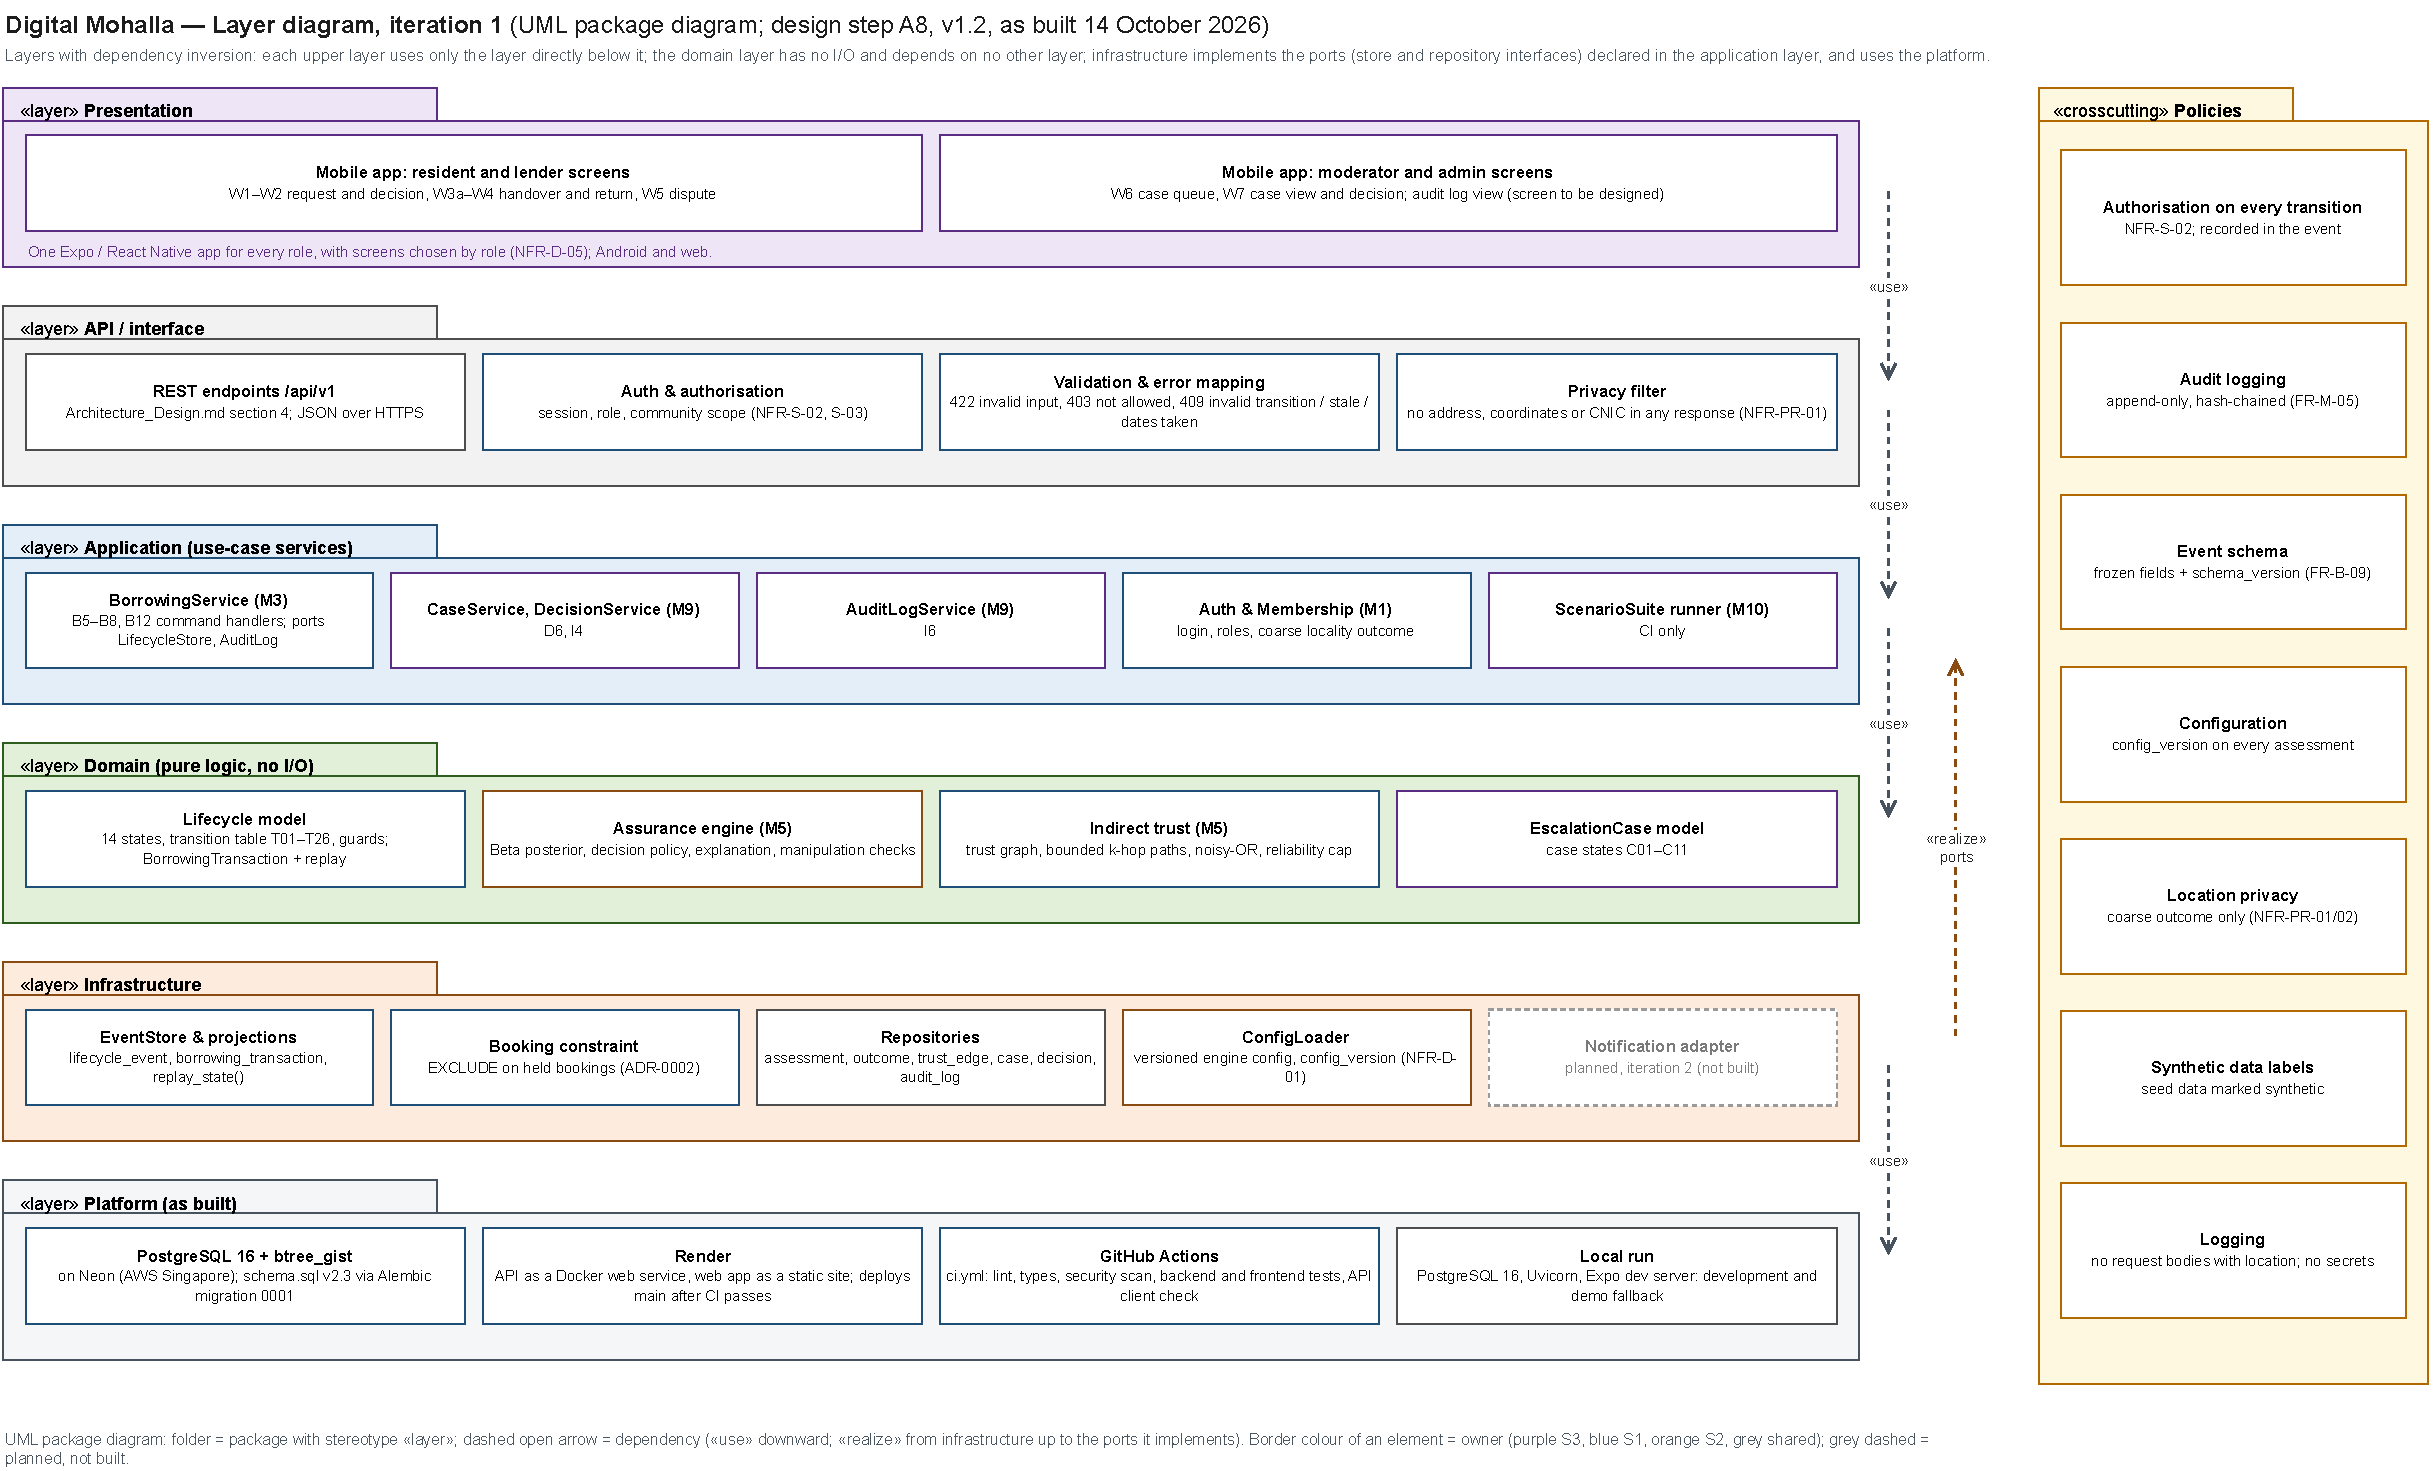
\includegraphics[width=\textwidth,height=0.80\textheight,keepaspectratio]{figures/diagrams/layer_diagram}
\caption{Layer diagram, Iteration 1 (UML package diagram, design step A8)}\label{fig:layer-diagram}
\drawionote{layer_diagram}{docs/design/03_architecture/layer_diagram.drawio}
\end{figure}

\textbf{Reasoning.} Each upper layer depends only on the one below it, and infrastructure depends upward on the ports it implements. The \textit{domain} layer (lifecycle model, assurance engine, moderation rules) is pure Python with no input/output, so the trust maths and the decision rules can be unit-tested without a database (477 unit tests run in seconds). Repositories are declared as interfaces in the application layer and implemented in infrastructure (dependency inversion), which is why the engine reaches the database only through the \code{EvidenceSource} interface. A monolith was chosen over services because three developers and one database do not need network boundaries, and a single transaction must cover the lifecycle transition, the booking and the event (ADR-0002). Cross-cutting policies (authorisation on every transition, the frozen event schema, \code{config_version} on every assessment, location privacy, synthetic labels) apply to every layer. \textit{Serves:} NFR-D-01, NFR-D-04, NFR-S-02, NFR-PR-01. \textit{Owner:} S1. The platform layer shows the deployed platform, Render and Neon (Section~\ref{sec:deployment}); the provisional AWS host of Part A is recorded in Section~\ref{sec:design-evolution}.

\section{Architectural Components}\label{sec:architectural-components}
Figure~\ref{fig:component-diagram} shows the ten modules, with the five worked on in Iteration 1 in detail.

\begin{figure}[p]
\centering
\begin{minipage}[c][0.92\textheight][c]{\textwidth}\centering
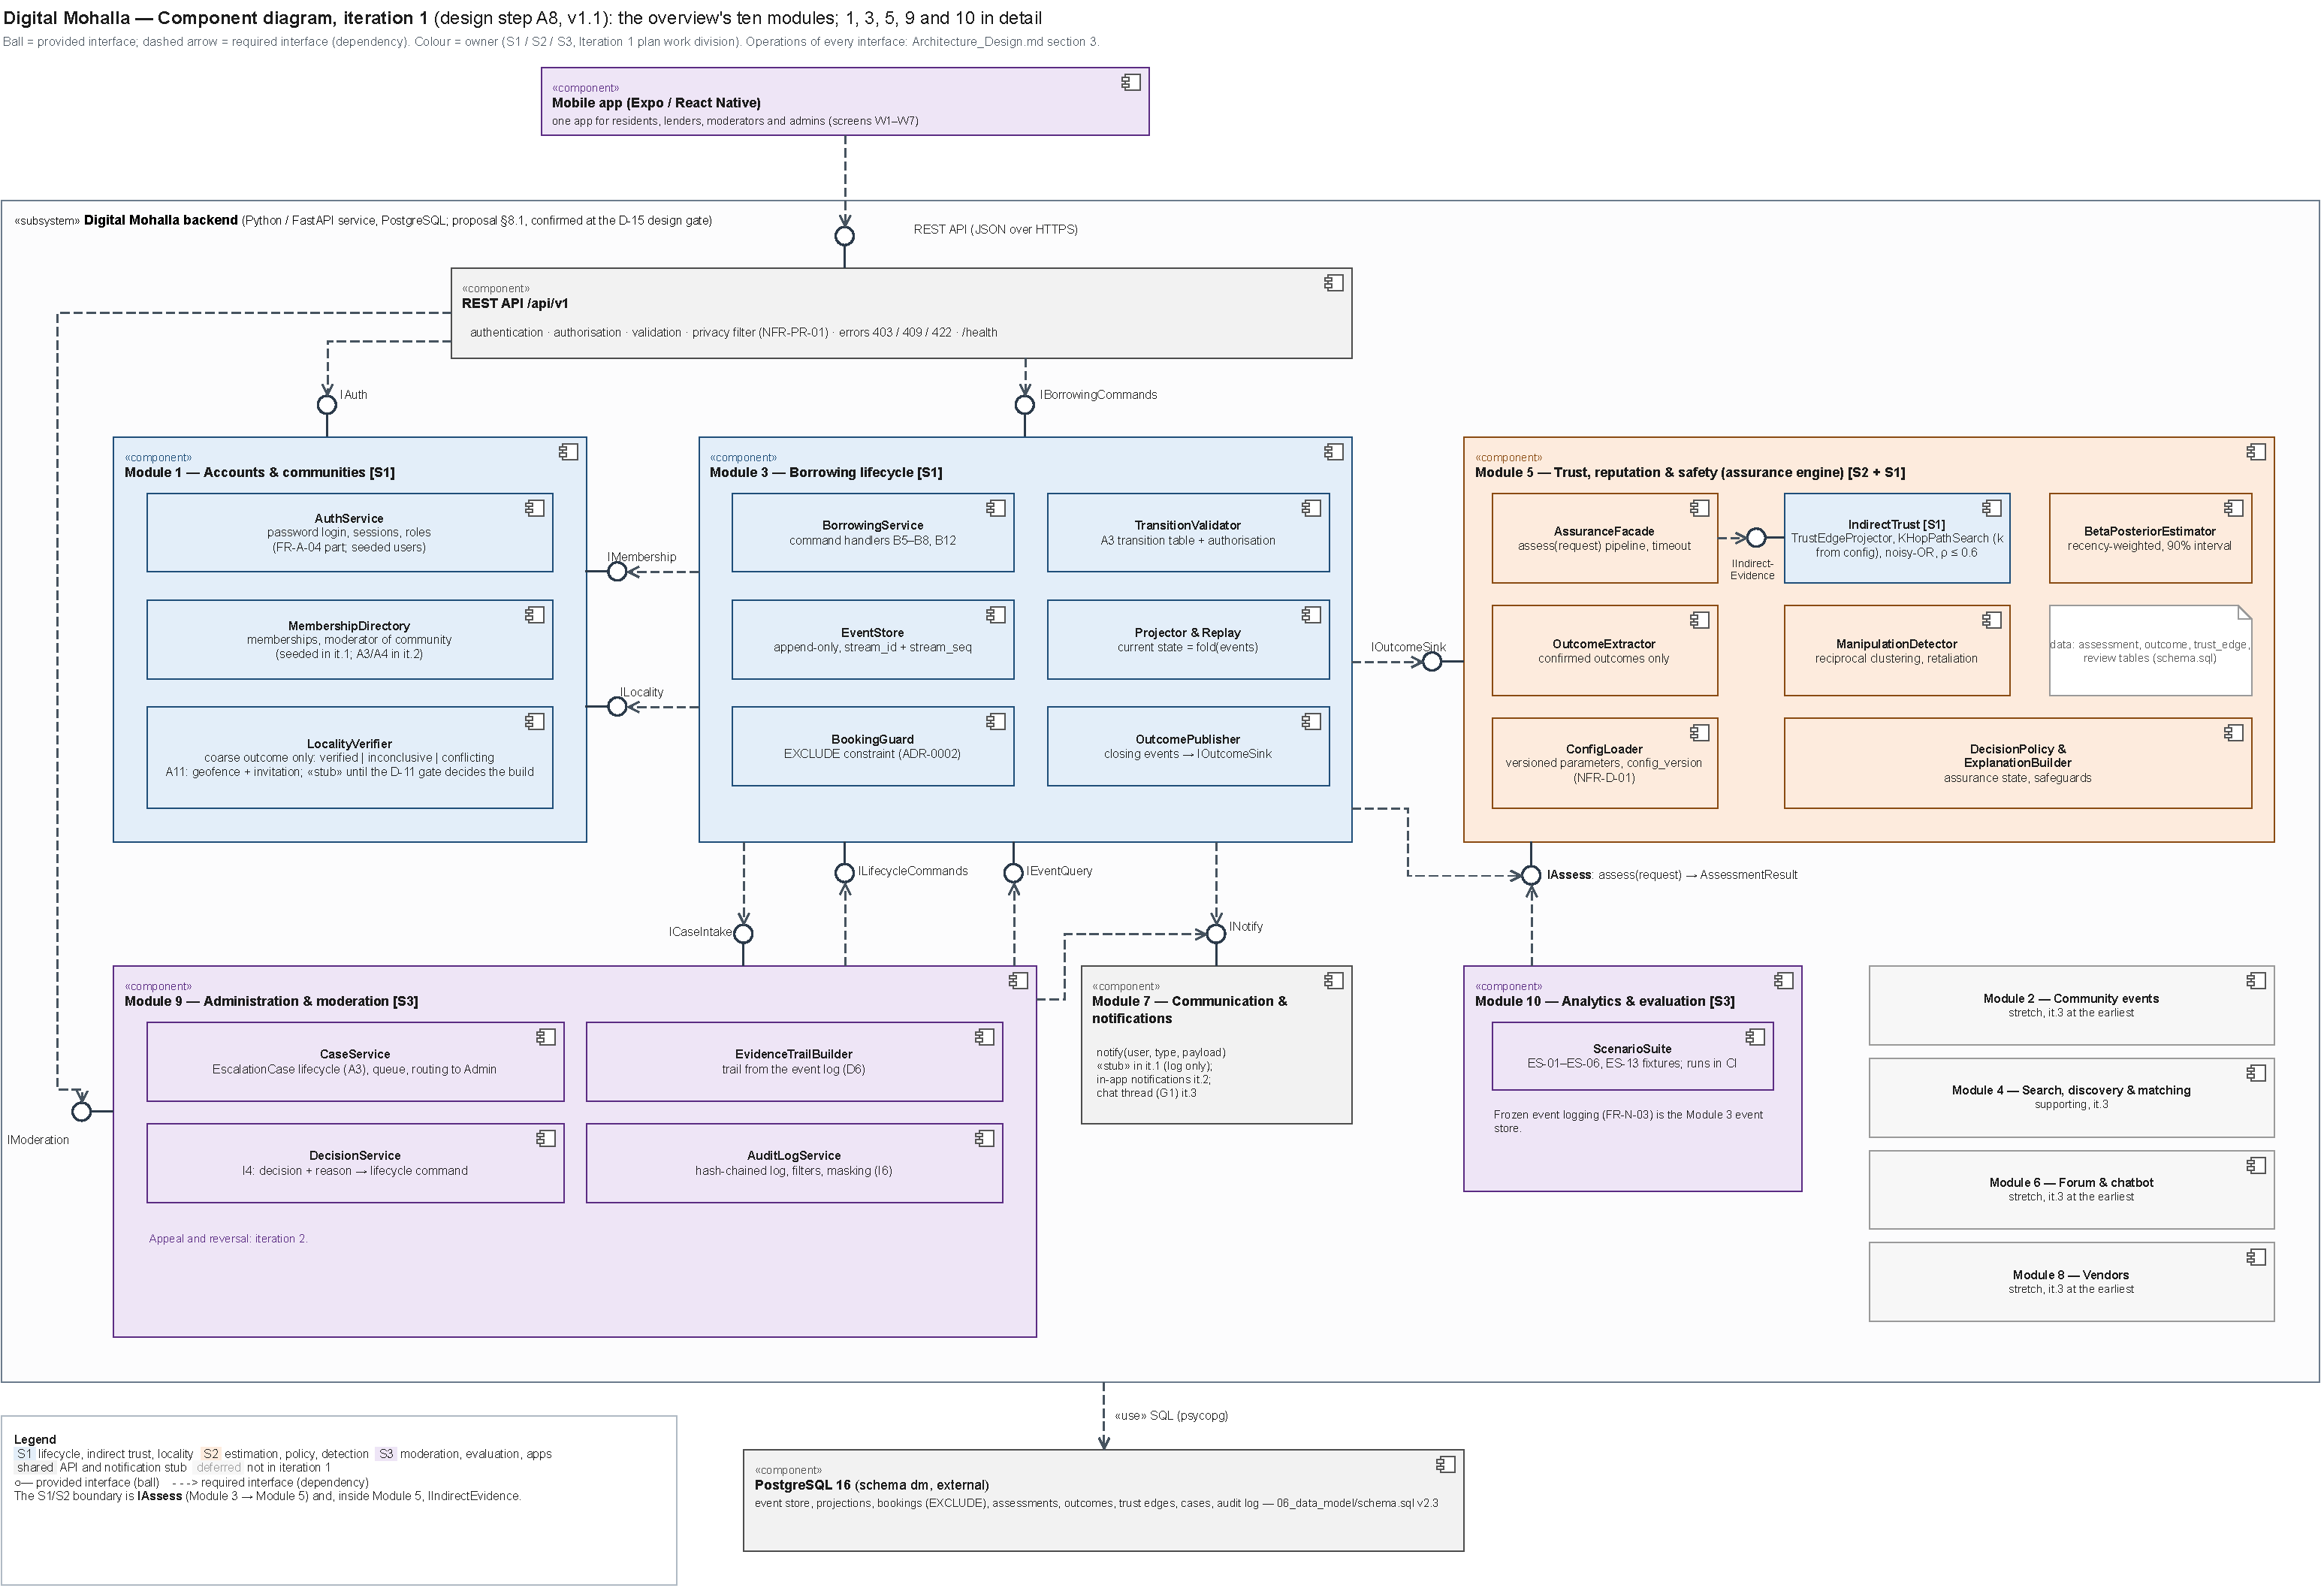
\includegraphics[width=\textwidth,height=0.80\textheight,keepaspectratio]{figures/diagrams/component_diagram}
\caption{Component diagram, Iteration 1 (UML 2.5, design step A8). Colour shows the owner (S1 blue, S2 orange, S3 purple)}\label{fig:component-diagram}
\drawionote{component_diagram}{docs/design/03_architecture/component_diagram.drawio}
\end{minipage}
\end{figure}

\textbf{Reasoning.} The diagram makes ownership and boundaries visible. Module 3 (lifecycle) and Module 5 (assurance) meet at exactly one provided interface, \code{IAssess.assess(request)}; inside Module 5 the S1/S2 boundary is the indirect-evidence interface. Module 3 calls the engine once per request, so a slow or failing engine affects one request and is turned into a hold (FR-T-07) instead of an error. Moderation (Module 9) changes the lifecycle only through lifecycle commands, so a moderator's decision passes the same transition checks as any other actor's. Modules 2, 4, 6 and 8 are drawn as deferred so the scope boundary is explicit. \textit{Serves:} FR-T-01, FR-T-07, FR-T-11, FR-B-08.

\textbf{From design components to code.} During implementation several design classes became plain functions or merged into one service, because Python modules and protocols gave the same boundaries with less code. Table~\ref{tab:design-components-mapped-implementation} maps every component in Figure~\ref{fig:component-diagram} to the code that realises it.

\begingroup\small
\begin{longtable}{@{}L{111pt}L{149pt}L{115pt}@{}}
\caption{Design components mapped to the implementation}\label{tab:design-components-mapped-implementation}\\
\toprule
Design element (A7/A8) & Implementation & Note \\
\midrule
\endfirsthead
\toprule
Design element (A7/A8) & Implementation & Note \\
\midrule
\endhead
\bottomrule
\endlastfoot
\code{IAssess} & \code{IAssess} protocol, \code{domain/lifecycle/ports.py} & As designed \\
\code{AssuranceFacade} & \code{AssuranceEngine.assess()}, \code{domain/assurance/engine.py} & Renamed \\
\code{BetaPosteriorEstimator} & \code{estimate()}, \code{credible_interval()}, \code{recency_weight()} in \code{estimation/posterior.py}; \code{similarity.py} & Functions instead of a class (pure) \\
\code{OutcomeExtractor}, \code{IOutcomeSink} & \code{estimation/outcomes.py} (rules) and \code{infra/db/outcomes.py} (writer), called from the close hook in \code{BorrowingService} & Interface replaced by a direct, idempotent call on loan close \\
\code{IndirectTrust}, \code{IIndirectEvidence}, \code{TrustEdgeProjector}, \code{KHopPathSearch} & \code{indirect/khop.py} (\code{find_paths}, \code{indirect_trust}), \code{indirect/edges.py}, \code{infra/db/trust_edges.py} & S1/S2 boundary kept as a module boundary \\
\code{ManipulationDetector}, \code{ReciprocalClustering}, \code{ReviewSimilarity}, \code{RetaliationCheck} & \code{detection/manipulation.py}: \code{partner_clustering}, \code{review_similarity}, retaliation set-aside, \code{combine} & S1 redefined as partner clustering (D18) \\
\code{DecisionPolicy}, \code{ExplanationBuilder} & \code{policy/decision.py} (\code{decide}, \code{RULES}), \code{policy/explanation.py} & As designed \\
\code{ConfigLoader} & \code{config/engine_config.py}, \code{config/engine.json} & As designed \\
\code{BorrowingService} & \code{BorrowingService}, \code{domain/lifecycle/service.py} & Also hosts dispute and moderation commands \\
\code{TransitionValidator} & \code{TransitionTable} (\code{transition_table.py}) and the database foreign key to \code{allowed_transition} & Checked twice \\
\code{EventStore}, \code{IEventQuery}, \code{Projector & Replay} & \code{LifecycleStore} protocol; \code{infra/eventstore/postgres.py}, \code{store.py}; \code{aggregate.py}; SQL \code{replay_state()} & As designed \\
\code{BookingGuard} & PostgreSQL exclusion constraint on \code{booking} & No Python class needed \\
\code{CaseService}, \code{DecisionService}, \code{ICaseIntake}, \code{IModeration} & \code{domain/moderation/decisions.py} (\code{plan}) and \code{BorrowingService.decide}, \code{moderation_queue}, \code{moderator_case} & Merged into the lifecycle service \\
\code{EvidenceTrailBuilder} & \code{BorrowingService.dispute_case}, \code{moderator_case} (trail read from \code{lifecycle_event}) & As designed \\
\code{AuditLogService} & \code{AuditLog} protocol; hash-chained \code{audit_log} table & Screen in Iteration 2 \\
\code{LocalityVerifier}, \code{ILocality} & \code{LifecycleStore.locality_outcome()} reading the stored result (\code{locality_outcome_for()}) & Stub; method in Iteration 2 \\
\code{INotify} & Not built & Iteration 2 \\
\code{AuthService}, \code{IAuth} & \code{domain/accounts/auth.py}, \code{api/deps.py} & Minimal login \\
\end{longtable}
\endgroup
\section{Interfaces and Dependencies}\label{sec:interfaces-dependencies}
\subsection{External interface: REST API}\label{sec:external-interface-rest-api}
The API is served under \code{/api/v1}, takes and returns JSON, and is described by an OpenAPI document from which the app's typed client is generated (a CI job fails if the two drift apart). Every request body refuses unknown fields, so a client cannot set the actor, the authorisation or the next state itself.

\begin{table}[!htbp]
\centering
\small
\caption{REST endpoints (Iteration 1)}\label{tab:rest-endpoints-iteration-1}
\begin{tabular}{@{}L{39pt}L{174pt}L{162pt}@{}}
\toprule
Method & Path & Purpose \\
\midrule
POST & \code{/auth/login} & Password login; returns a token \\
GET & \code{/items}, \code{/items/{id}} & Items visible to the member \\
POST & \code{/requests} & Create a borrowing request (UC-B5) \\
GET & \code{/requests}, \code{/requests/{id}}, \code{/lender/requests} & The member's requests; one request with its assessment; the lender's queue \\
POST & \code{/requests/{id}/accept}, \code{/decline}, \code{/cancel} & Lender decision; borrower cancellation (UC-B6) \\
POST & \code{/transactions/{id}/handover/checklist}, \code{/handover/confirm} & Handover (UC-B7) \\
POST & \code{/transactions/{id}/return}, \code{/return/confirm} & Return (UC-B8) \\
GET & \code{/transactions/{id}/events} & The event trail \\
POST, GET & \code{/transactions/{id}/dispute}, \code{/dispute/withdraw} & Raise, view and withdraw a dispute (UC-B12) \\
GET & \code{/moderation/cases}, \code{/moderation/cases/{id}} & Moderator queue and case view \\
POST & \code{/moderation/cases/{id}/decision} & Moderator decision with reason (UC-I4) \\
GET & \code{/health} & Liveness check for deployment \\
\bottomrule
\end{tabular}
\end{table}
Errors follow one mapping: 401 without a valid token, 403 for the wrong actor, 404 for data the member may not see, 409 for an invalid transition, a stale command or ``dates taken'', and 422 for invalid input.

\subsection{Internal interfaces}\label{sec:internal-interfaces}
\begin{itemize}
\item \code{IAssess.assess(AssessmentRequest) -> AssessmentResult}: the only way the lifecycle reaches the engine; called with a 2,000 ms timeout read from the configuration.
\item \code{LifecycleStore}: everything the lifecycle service needs from storage (create, append, view, assessments, cases, decisions, bookings), implemented on PostgreSQL.
\item \code{EvidenceSource}: what the engine reads (the borrower's outcomes, the trust graph, open and recent disputes, verification, reviews and complaints), so the engine itself has no database code.
\item \code{AuditLog}: records refused commands and privileged actions.
\end{itemize}

External dependencies are listed with versions and licences in Section~\ref{sec:external-components-dependencies}.

\section{Architecture Decisions and Rationale}\label{sec:architecture-decisions-rationale}
Eight ADRs record the decisions that shape the code. The hosting choice (Render and Neon instead of the provisional AWS host) is recorded as a design change (Table~\ref{tab:design-changes-since-proposal}); its ADR is pending. (\code{docs/design/03_architecture/DigitalMohalla_ADRs_Ver1.md}).

\begingroup
\begin{longtable}{@{}L{34pt}L{137pt}L{204pt}@{}}
\caption{Architecture decision records}\label{tab:architecture-decision-records}\\
\toprule
ADR & Decision & Rationale \\
\midrule
\endfirsthead
\toprule
ADR & Decision & Rationale \\
\midrule
\endhead
\bottomrule
\endlastfoot
0001 & Soft hold: pending requests mark dates as requested and block nothing & A lender should see all interest; blocking at request time would let one borrower lock an item with requests \\
0002 & The database enforces the no-overlap rule at acceptance (exclusion constraint on held bookings); transition, booking and event commit in one transaction & Replaces ``lower \code{stream_seq} wins'', which only orders events within one transaction and cannot arbitrate between two transactions \\
0003 & Exits from HELD\_FOR\_REVIEW depend on the hold reason (new event \code{hold_cleared}) & A cleared locality hold must still be assessed; a cleared manipulation hold already has an assessment; an engine-failure hold has nothing to attach safeguards to \\
0004 & Separate \code{dispute_resolved} and \code{dispute_withdrawn} events & A withdrawal restores the previous state; a resolution completes the loan and creates evidence; one event type could not mean both \\
0005 & Event-specific data goes in a \code{payload} field defined per event type & Keeps the frozen schema stable while each event carries its own data (dates, reasons, safeguards) \\
0006 & A trust edge's weight is the recency-weighted Beta posterior mean of the source's verified outcomes with the target (experimental) & One estimator for direct and indirect evidence; never a manual vouch \\
0007 & A manipulation hold needs corroboration (risk $\geq$60 and two signals $\geq$0.5); S4 active in Iteration 1 & ``$\geq$60 always holds'' contradicted the false-positive guard for real families; with one signal ES-04 could not be held at all \\
0008 & Community paths lift sparse direct evidence from INSUFFICIENT to REVIEW\_RECOMMENDED, never to SUFFICIENT & Without it the indirect evidence could never change a decision \\
\end{longtable}
\endgroup
Team decisions record the smaller choices: D1--D9 on 11 October (for example the \code{payload} field, no disputes from RETURNED, merging the Request table into the transaction) and D10--D20 on 13 October (Table~\ref{tab:team-decisions-d10-d20}).

\begingroup
\begin{longtable}{@{}L{26pt}L{136pt}L{213pt}@{}}
\caption{Team decisions D10--D20 (13 October 2026)}\label{tab:team-decisions-d10-d20}\\
\toprule
\# & Topic & Decision \\
\midrule
\endfirsthead
\toprule
\# & Topic & Decision \\
\midrule
\endhead
\bottomrule
\endlastfoot
D10 & Trust-edge weight & ADR-0006 accepted as experimental \\
D11 & Outcome mapping & Borrower: on-time return, condition agreed, dispute-free; lender: condition agreed, dispute-free; a party found at fault fails the relevant metrics \\
D12 & SUFFICIENT\_EVIDENCE thresholds & Mean $\geq 0.75$, lower 90\% bound $\geq 0.60$, $n_{\mathrm{eff}} \geq 3$, $\rho_{\mathrm{sup}} = 0.3$: initial hypotheses \\
D13 & ES-05 expected result & R8, SUFFICIENT\_EVIDENCE with safeguards: the retaliatory review is detected and set aside \\
D14 & ES-13 expected result & R9, REVIEW\_RECOMMENDED; without the community paths, R6\_SPARSE \\
D15 & Device scope & Android only for device testing; iOS not targeted \\
D16 & Test plan use & Tools added only when a test first needs them \\
D17 & Similarity of a past loan & $0.4\times$ value-band closeness $+\,0.4\times$ same category $+\,0.2\times$ duration closeness, floor 0.5 (S2) \\
D18 & Meaning of S1 & Partner clustering instead of pairwise reciprocity (confirmed by S2, 14 October) \\
D19 & Effect of a retaliation flag & The review is set aside from S1 and S4 and explained; reviews never enter the trust estimate (confirmed by S2, 14 October) \\
D20 & Photo uploads & Deferred to Iteration 2 (confirmed by S1 and S2, 14 October) \\
\end{longtable}
\endgroup
\section{Design Evolution}\label{sec:design-evolution}
\begingroup
\begin{longtable}{@{}L{111pt}L{111pt}L{153pt}@{}}
\caption{Design changes since the proposal}\label{tab:design-changes-since-proposal}\\
\toprule
Proposal / earlier design & Now & Why \\
\midrule
\endfirsthead
\toprule
Proposal / earlier design & Now & Why \\
\midrule
\endhead
\bottomrule
\endlastfoot
Nine technical components M1--M9 across a broad platform & Ten modules; the assurance engine is the core, stretch modules deferred & Panel point 3; the handbook's scope test needs a technical core per student \\
Trust shared by all three students & S1 indirect trust, S2 estimation/policy/detection, S3 moderation/evaluation & Each member owns a removable technical part \\
FAISS search, learning-to-rank, LightGBM & Search in Iteration 3; detection is rule-based and interpretable & No labelled data for a trained detector; every signal must be explainable to a moderator \\
Four reputation tiers & Four assurance states that describe evidence, not people & A tier labels a person; a state describes this loan's evidence \\
``Lower \code{stream_seq} wins'' for double booking & Database exclusion constraint (ADR-0002) & Correct across transactions and atomic \\
``RESUME'' to end a dispute & \code{dispute_resolved} / \code{dispute_withdrawn} (ADR-0004) & Different outcomes need different events \\
Separate Request table & Merged into \code{borrowing_transaction} (D7) & One stream per loan from request to close \\
Any risk $\geq$60 holds & Two corroborating signals needed (ADR-0007) & Protects real families (C3 guard) \\
Indirect evidence with no effect on the decision & R6\_SPARSE / R9 (ADR-0008) & Makes ES-13 decidable \\
Pairwise reciprocity signal & Partner clustering (D18) & Two-sided reviews are reciprocal by nature; the pairwise rule flagged 6 of 8 ordinary members \\
GPS sent with every request & Request carries no location; membership-time result is read (D13) & Privacy boundary moves to joining a community \\
One AWS host with Docker Compose (A13, provisional) & Render (API container and static web app) with Neon PostgreSQL & No server administration; deploys from \code{main} after CI \\
Design interfaces such as \code{IOutcomeSink}, \code{IIndirectEvidence} & Four protocols (\code{IAssess}, \code{LifecycleStore}, \code{EvidenceSource}, \code{AuditLog}) & Same boundaries, less code (Table~\ref{tab:design-components-mapped-implementation}) \\
\end{longtable}
\endgroup
\section{Domain Model}\label{sec:domain-model}
\textbf{Reasoning.} The central class is the \textit{BorrowingTransaction}, whose state is derived from its \textit{LifecycleEvents}; an \textit{Assessment} is attached to a transaction, not to a user, because an assurance state describes the evidence for one loan. \textit{Outcome} is separate from \textit{Review}: trust is computed only from verified outcomes, and reviews feed only the manipulation signals (D19), which is why a retaliatory review cannot lower anyone's trust. \textit{Booking}, \textit{ConditionReport} and \textit{LocalityResult} were kept as classes (integration decision of 11 October) because each is realised by a table and guarded by a database rule. \textit{Serves:} FR-B-09, FR-T-01, FR-T-03, FR-T-09.

\begin{figure}[p]
\centering
\begin{minipage}[c][0.92\textheight][c]{\textwidth}\centering
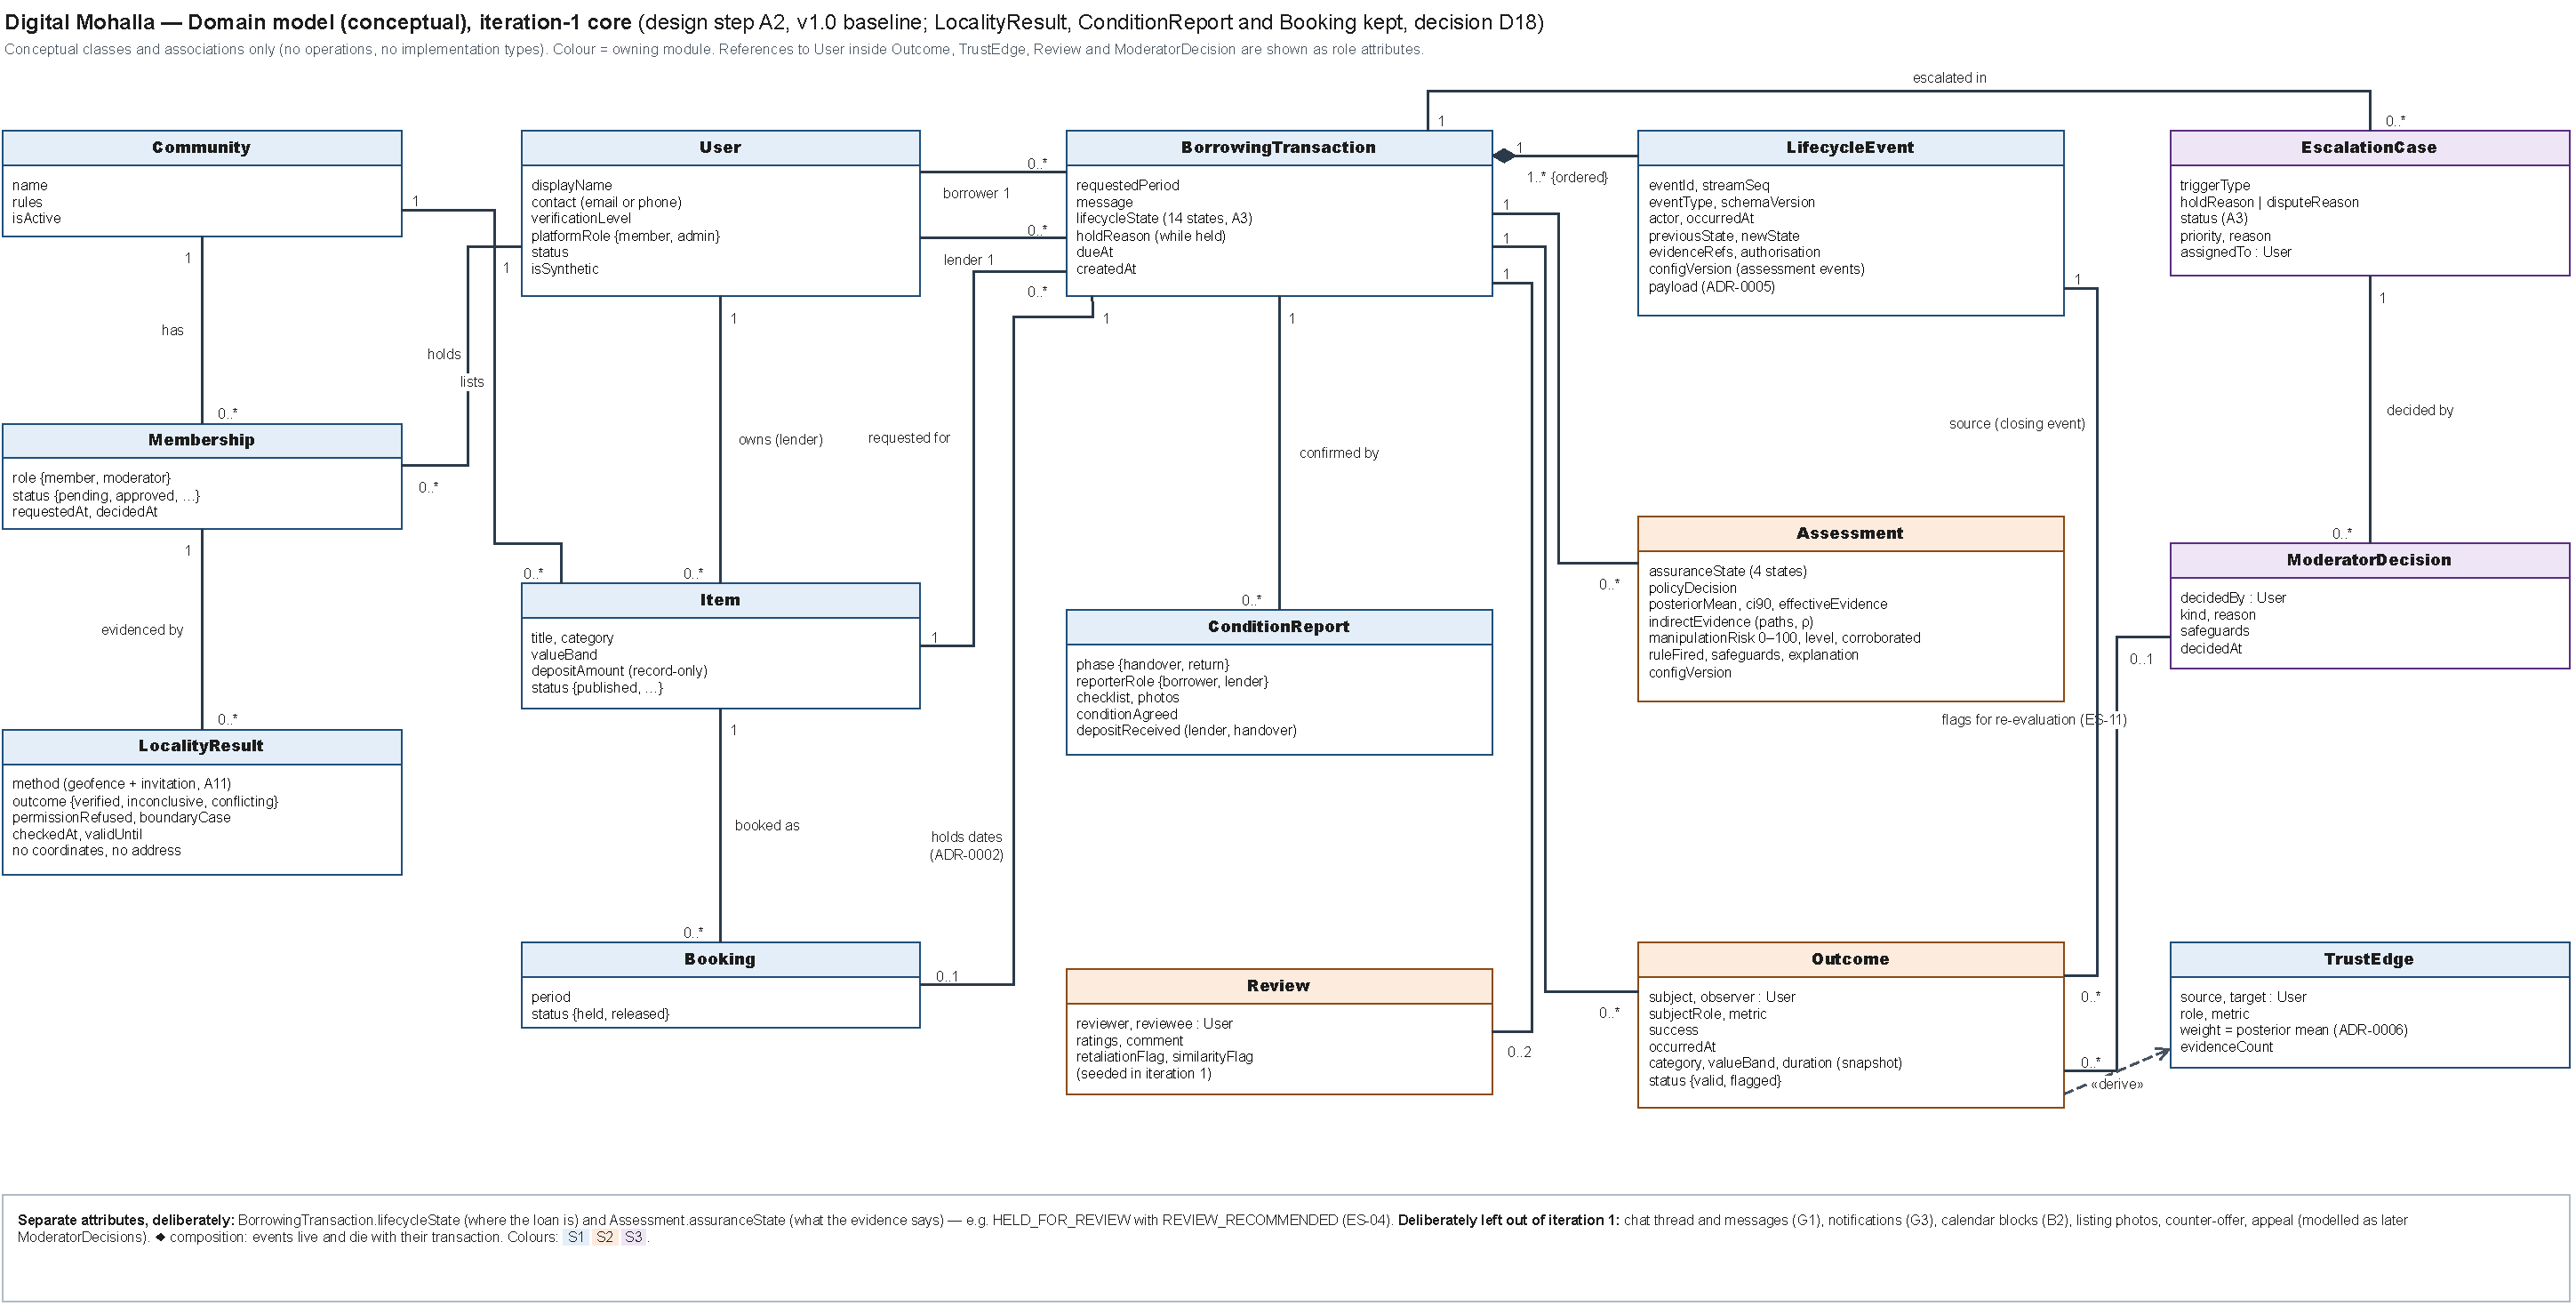
\includegraphics[width=\textwidth,height=0.80\textheight,keepaspectratio]{figures/diagrams/domain_model}
\caption{Domain model v1.0 (UML class diagram without operations, design step A2)}\label{fig:domain-model}
\drawionote{domain_model}{docs/design/05_class_model/domain_model.drawio}
\end{minipage}
\end{figure}

\section{Data Design}\label{sec:data-design}
\textbf{Reasoning.} The schema (\code{schema.sql} v2.3, applied by Alembic migration \code{0001}) enforces the rules that must never depend on application code:

\begin{itemize}
\item \textbf{Event store.} \code{lifecycle_event} is append-only (a trigger refuses UPDATE and DELETE) and hash-chained (\code{prev_hash}, \code{row_hash}); \code{verify_event_chain()} detects any altered row. \code{(stream_id, stream_seq)} is unique.
\item \textbf{Valid transitions.} \code{(previous_state, event_type, new_state)} is a composite foreign key to \code{allowed_transition}, so an invalid transition cannot be stored even if the Python check had a bug. The trigger \code{event_validate} checks the actor and sequence; \code{event_apply} updates the projection.
\item \textbf{Bookings.} \code{EXCLUDE (item_id WITH =, period WITH &&) WHERE held}, using \code{btree_gist}.
\item \textbf{Assessments.} Every row stores \code{config_version} (NOT NULL); \code{assessment_rule_ck} refuses a row whose rule, state, decision and hold reason disagree with the decision table.
\item \textbf{Privacy.} No column stores coordinates, an address or a CNIC; a test scans the catalogue for such columns.
\end{itemize}

\begin{figure}[p]
\centering
\begin{minipage}[c][0.92\textheight][c]{\textwidth}\centering
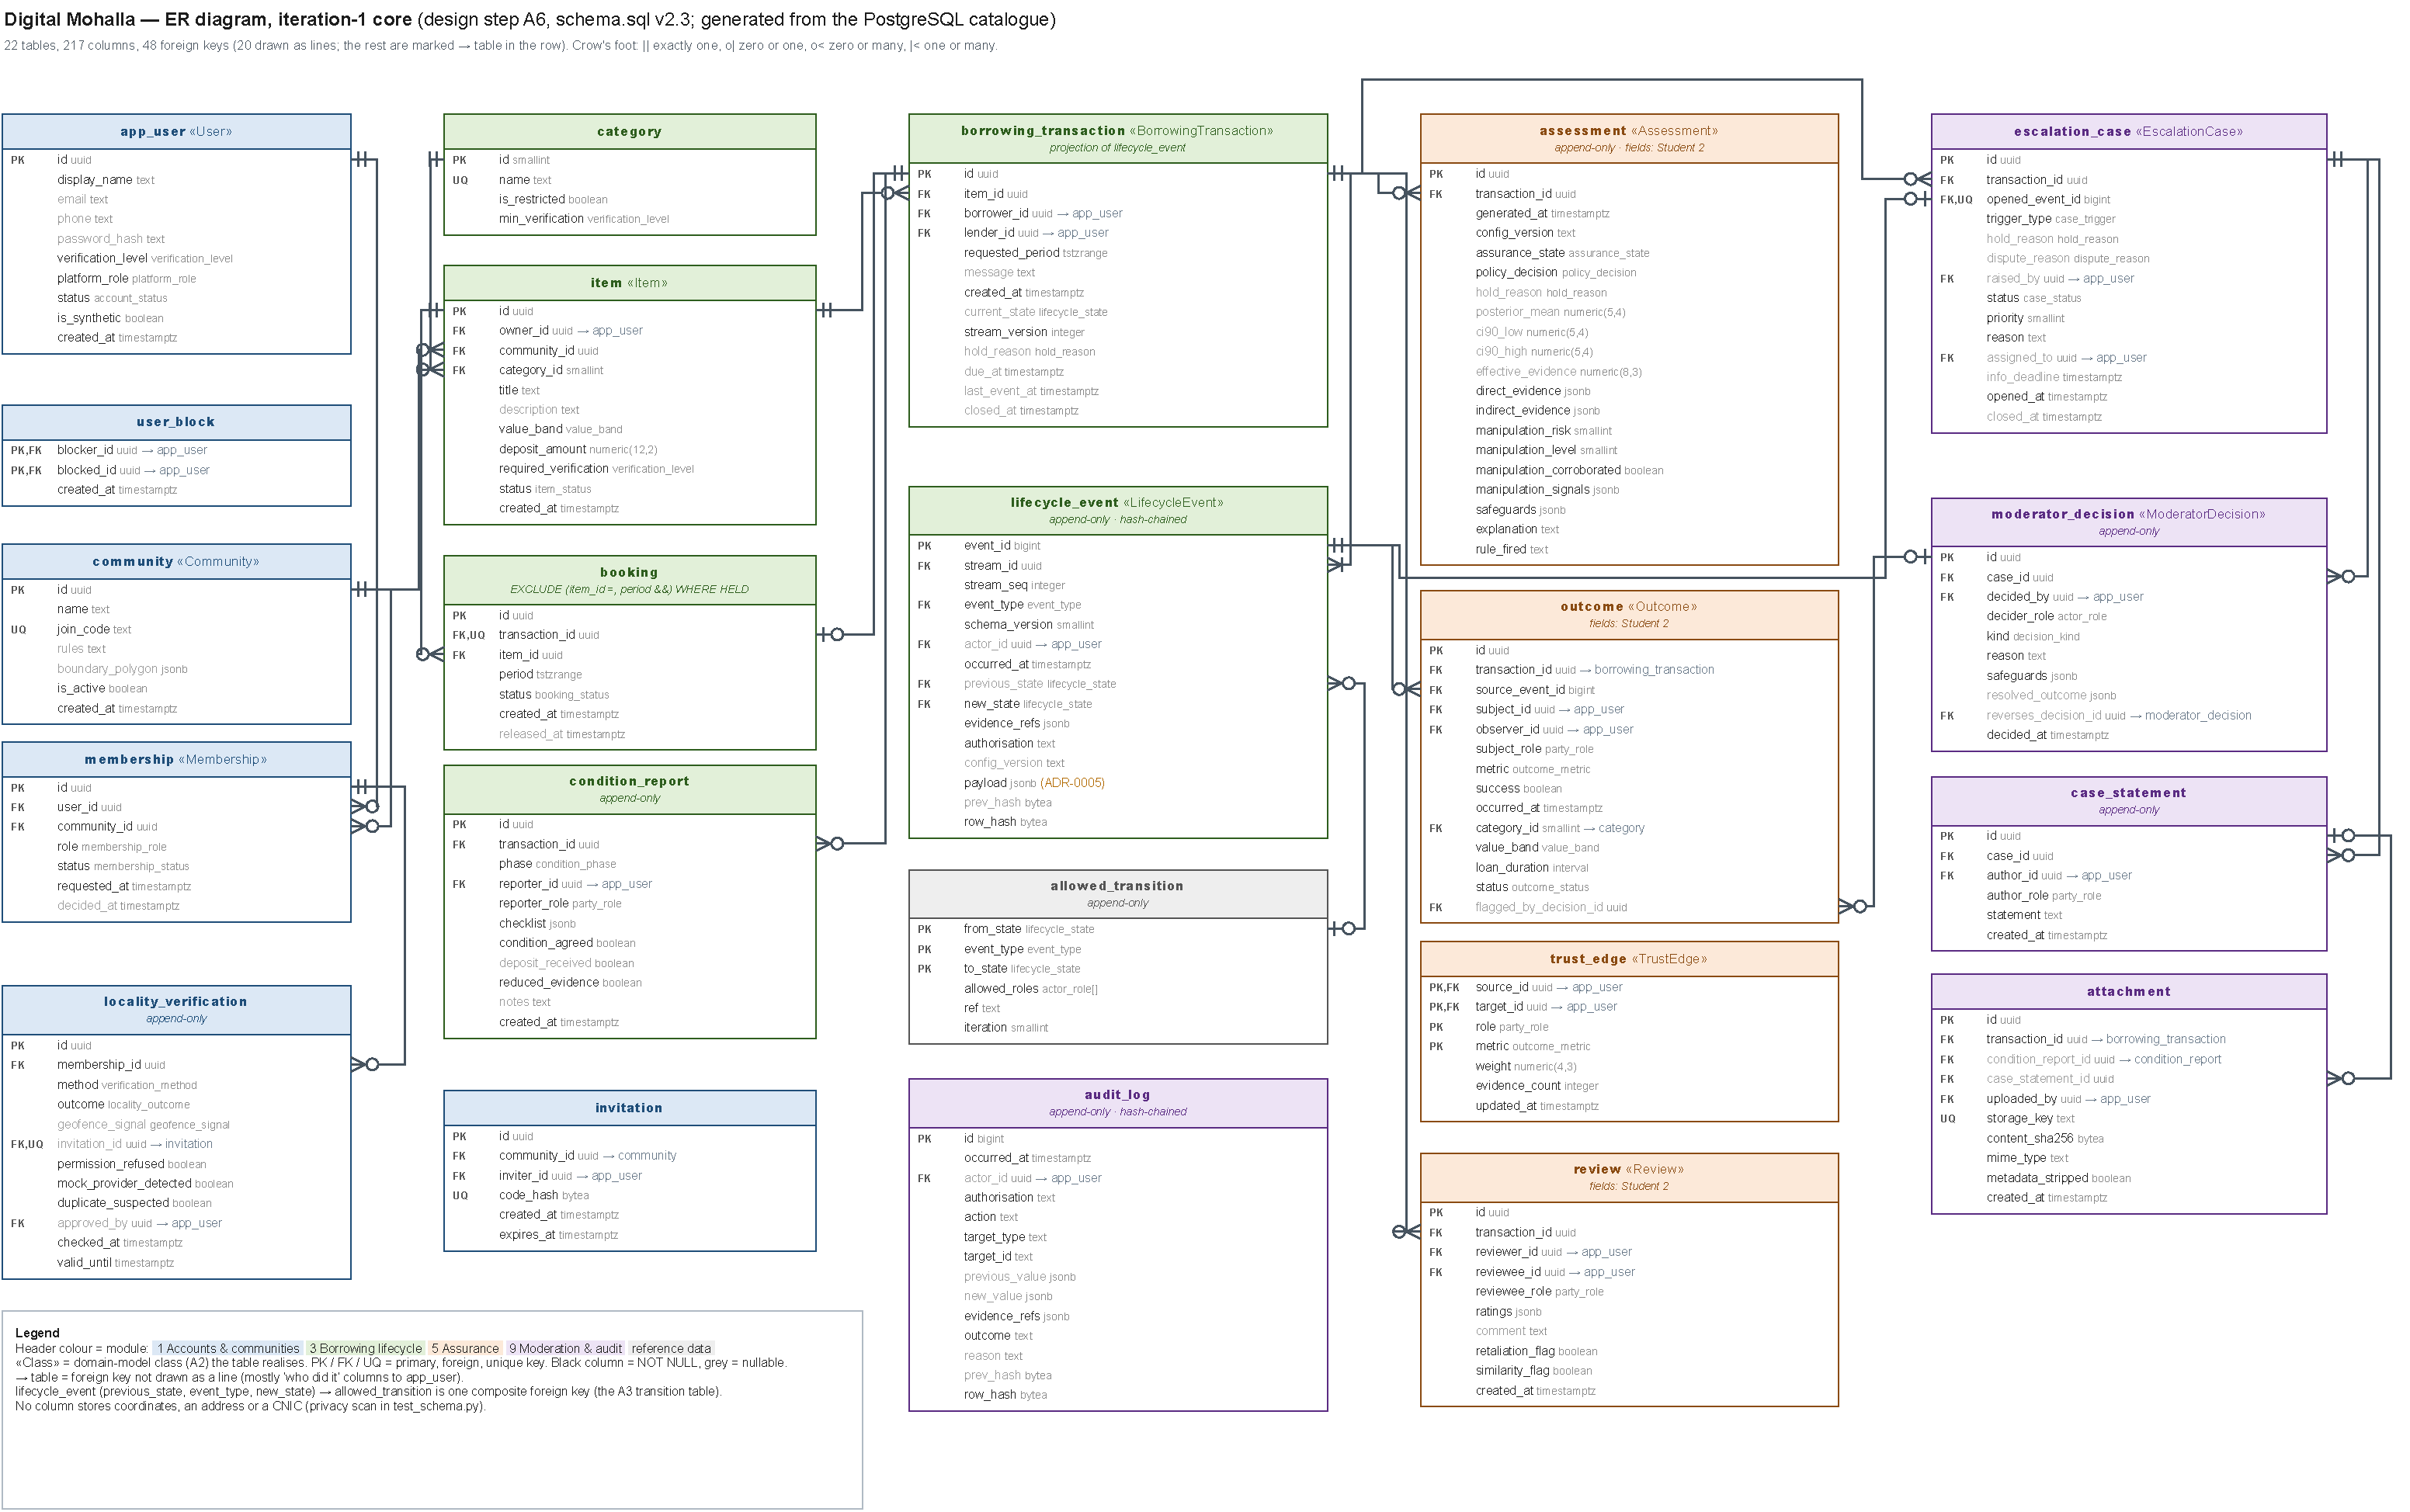
\includegraphics[width=\textwidth,height=0.80\textheight,keepaspectratio]{figures/diagrams/er_diagram}
\caption{ER diagram, schema v2.3 (crow's foot, design step A6): 22 tables, 217 columns, 48 foreign keys}\label{fig:er-diagram}
\drawionote{er_diagram}{docs/design/06_data_model/er_diagram.drawio}
\end{minipage}
\end{figure}

The current state is a projection (\code{borrowing_transaction.current_state}) that \code{replay_state()} can rebuild from the events alone. \textit{Serves:} FR-B-05, FR-B-08, FR-B-09, FR-M-05, NFR-D-01, NFR-PR-01. \textit{Owner:} S1 (lifecycle tables), S2 (assessment, outcome, trust edge, review fields).

\section{Process / Behavior Design}\label{sec:process-behavior-design}
\subsection{Borrowing lifecycle}\label{sec:borrowing-lifecycle}
\textbf{Reasoning.} Fourteen states in two composites: PENDING (dates only requested) and IN\_PROGRESS (booking held). Transitions that apply to every substate of a composite are drawn once on its border, and DISPUTED returns through a shallow-history state to the state stored in \code{dispute_opened}. HELD\_FOR\_REVIEW is never an automatic rejection: each hold reason has its own exits (ADR-0003). With the 21 event types this gives 294 state--event pairs, of which 31 are valid; the 31 valid pairs yield 34 leaf transitions because some events have guarded alternatives (for example \code{hold_cleared} returns to LOCALITY\_CHECKED or ASSESSED depending on the hold reason). Transitions marked ``it.2'' (expiry, no-show, extensions) are part of the table but are triggered by the Iteration 2 scheduler. \textit{Serves:} FR-B-08, FR-B-16, FR-B-17, FR-T-07.

\begin{figure}[p]
\centering
\begin{minipage}[c][0.92\textheight][c]{\textwidth}\centering
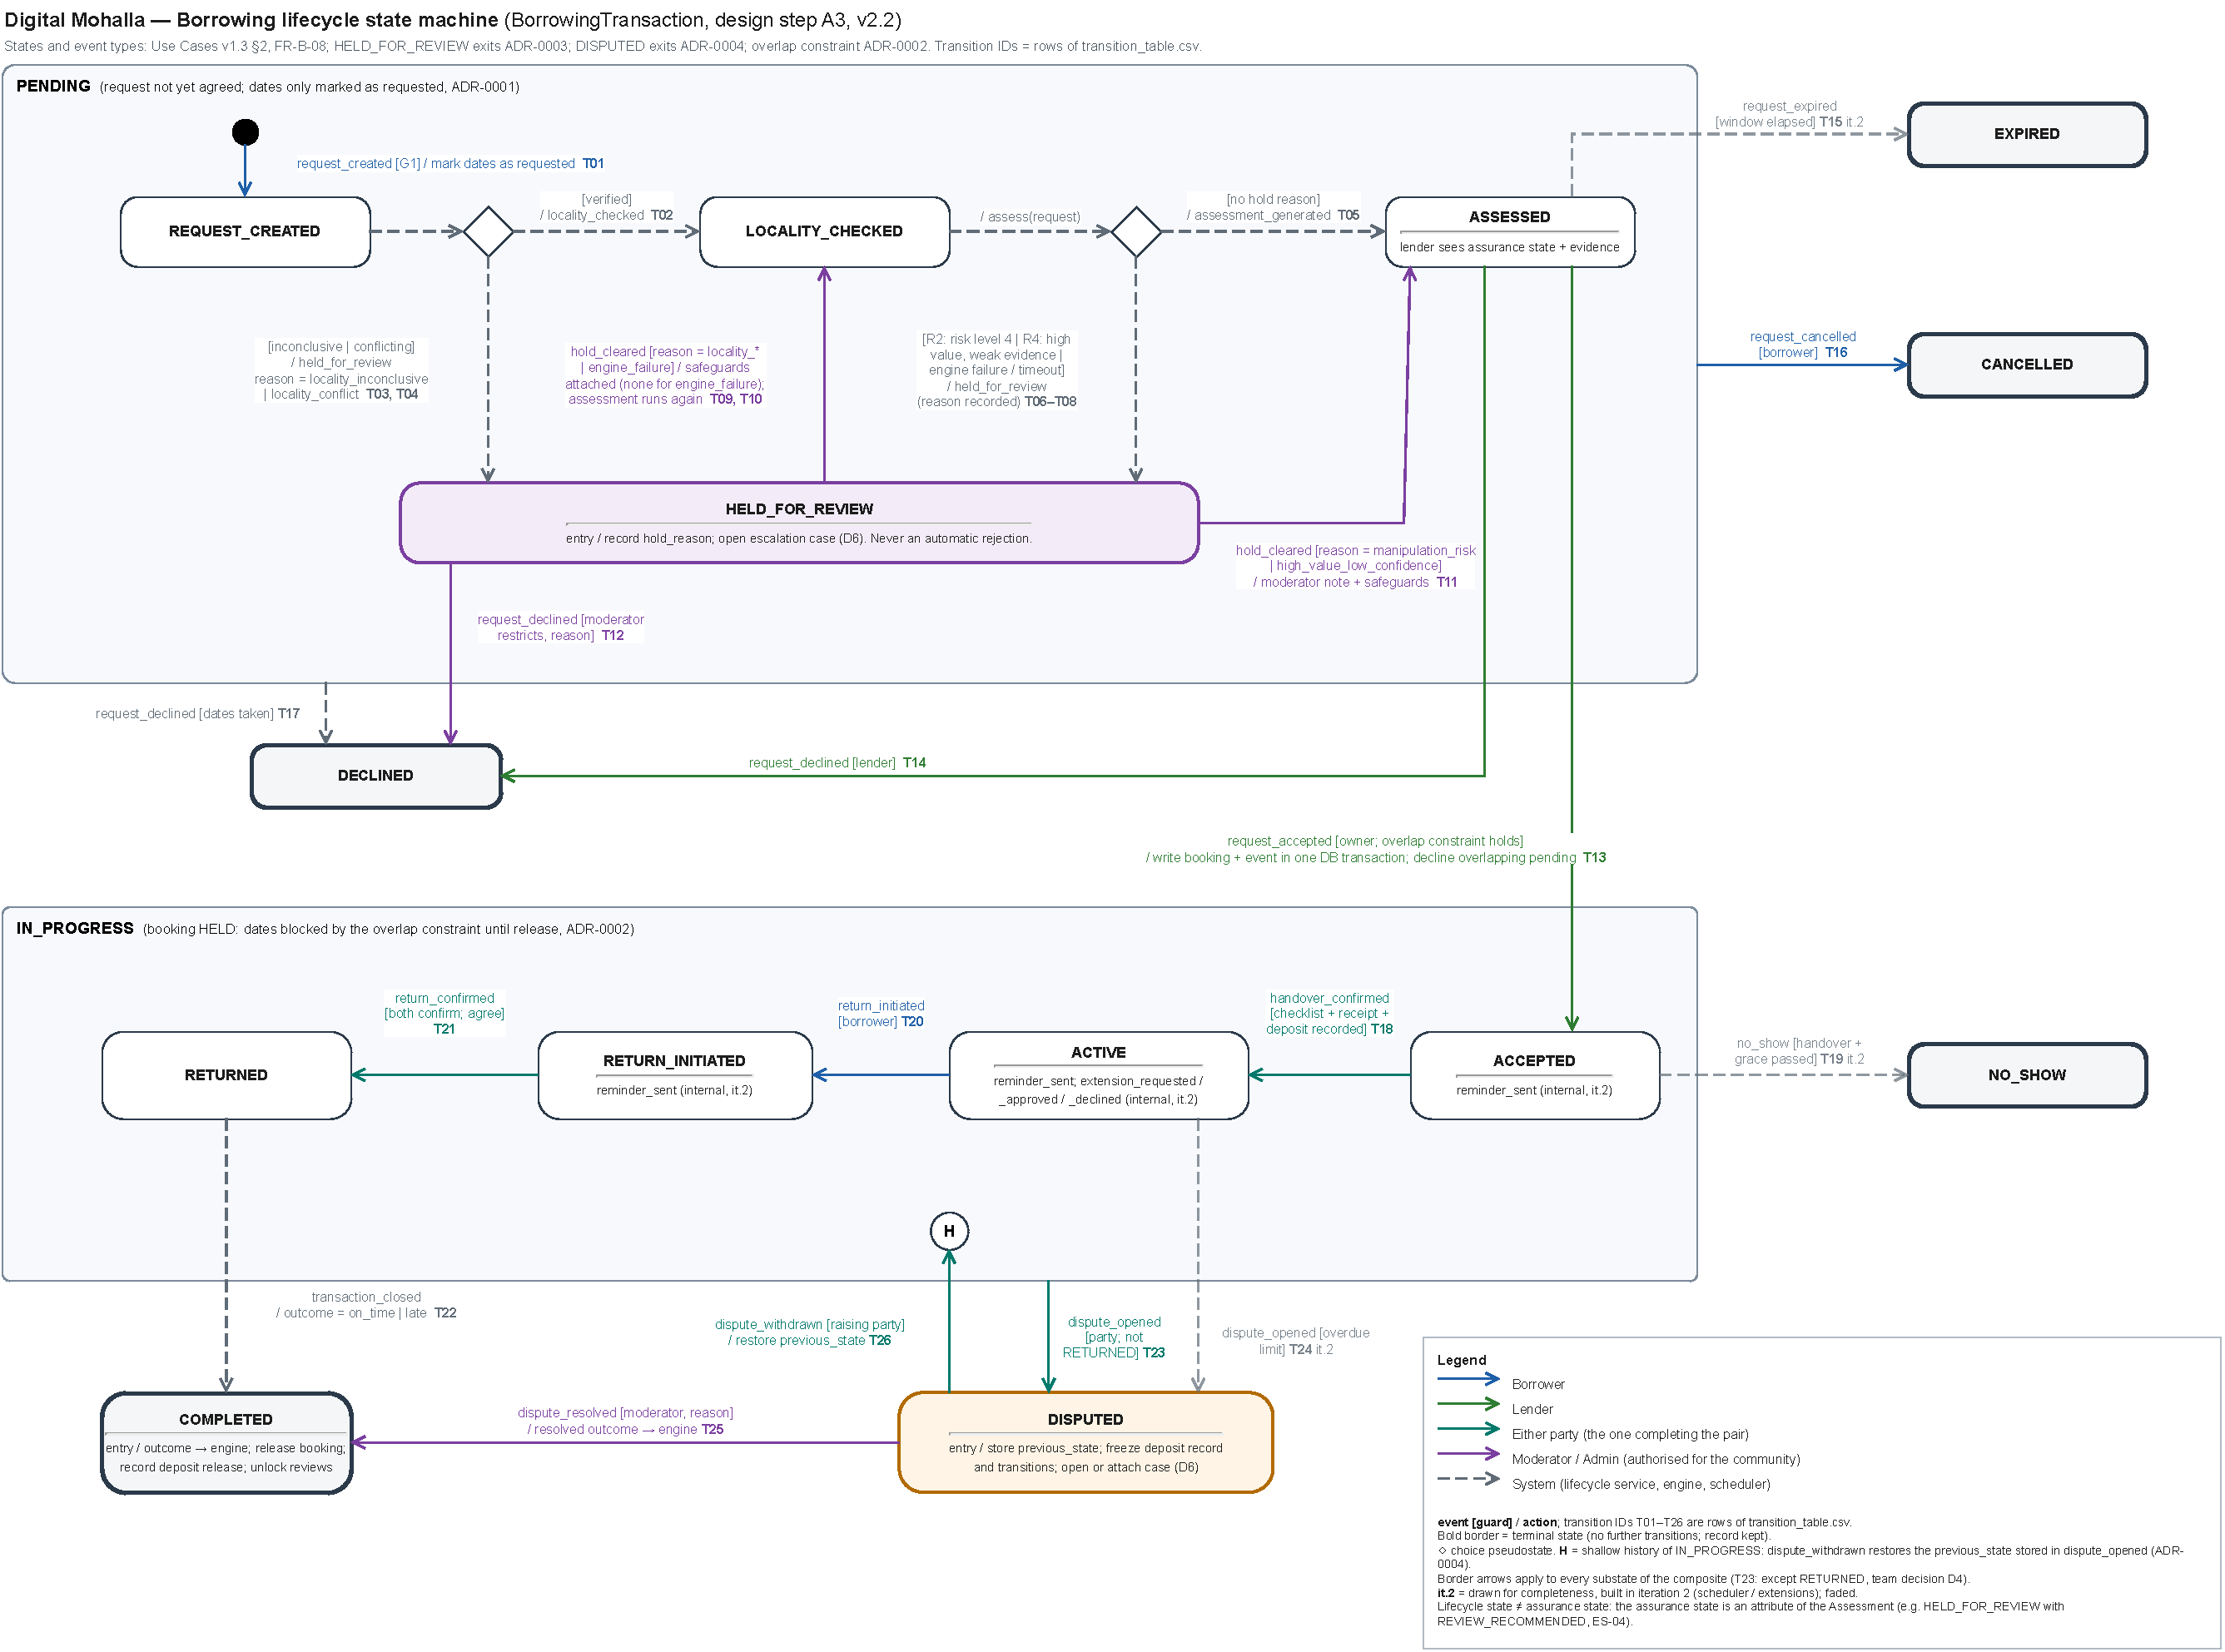
\includegraphics[width=\textwidth,height=0.80\textheight,keepaspectratio]{figures/diagrams/borrowing_lifecycle_state_machine}
\caption{Borrowing lifecycle state machine v2.2 (UML 2.5, design step A3)}\label{fig:borrowing-lifecycle-state-machine}
\drawionote{borrowing_lifecycle_state_machine}{docs/design/07_state_machines/borrowing_lifecycle_state_machine.drawio}
\end{minipage}
\end{figure}

\subsection{Escalation case}\label{sec:escalation-case}
\begin{figure}[htbp]
\centering
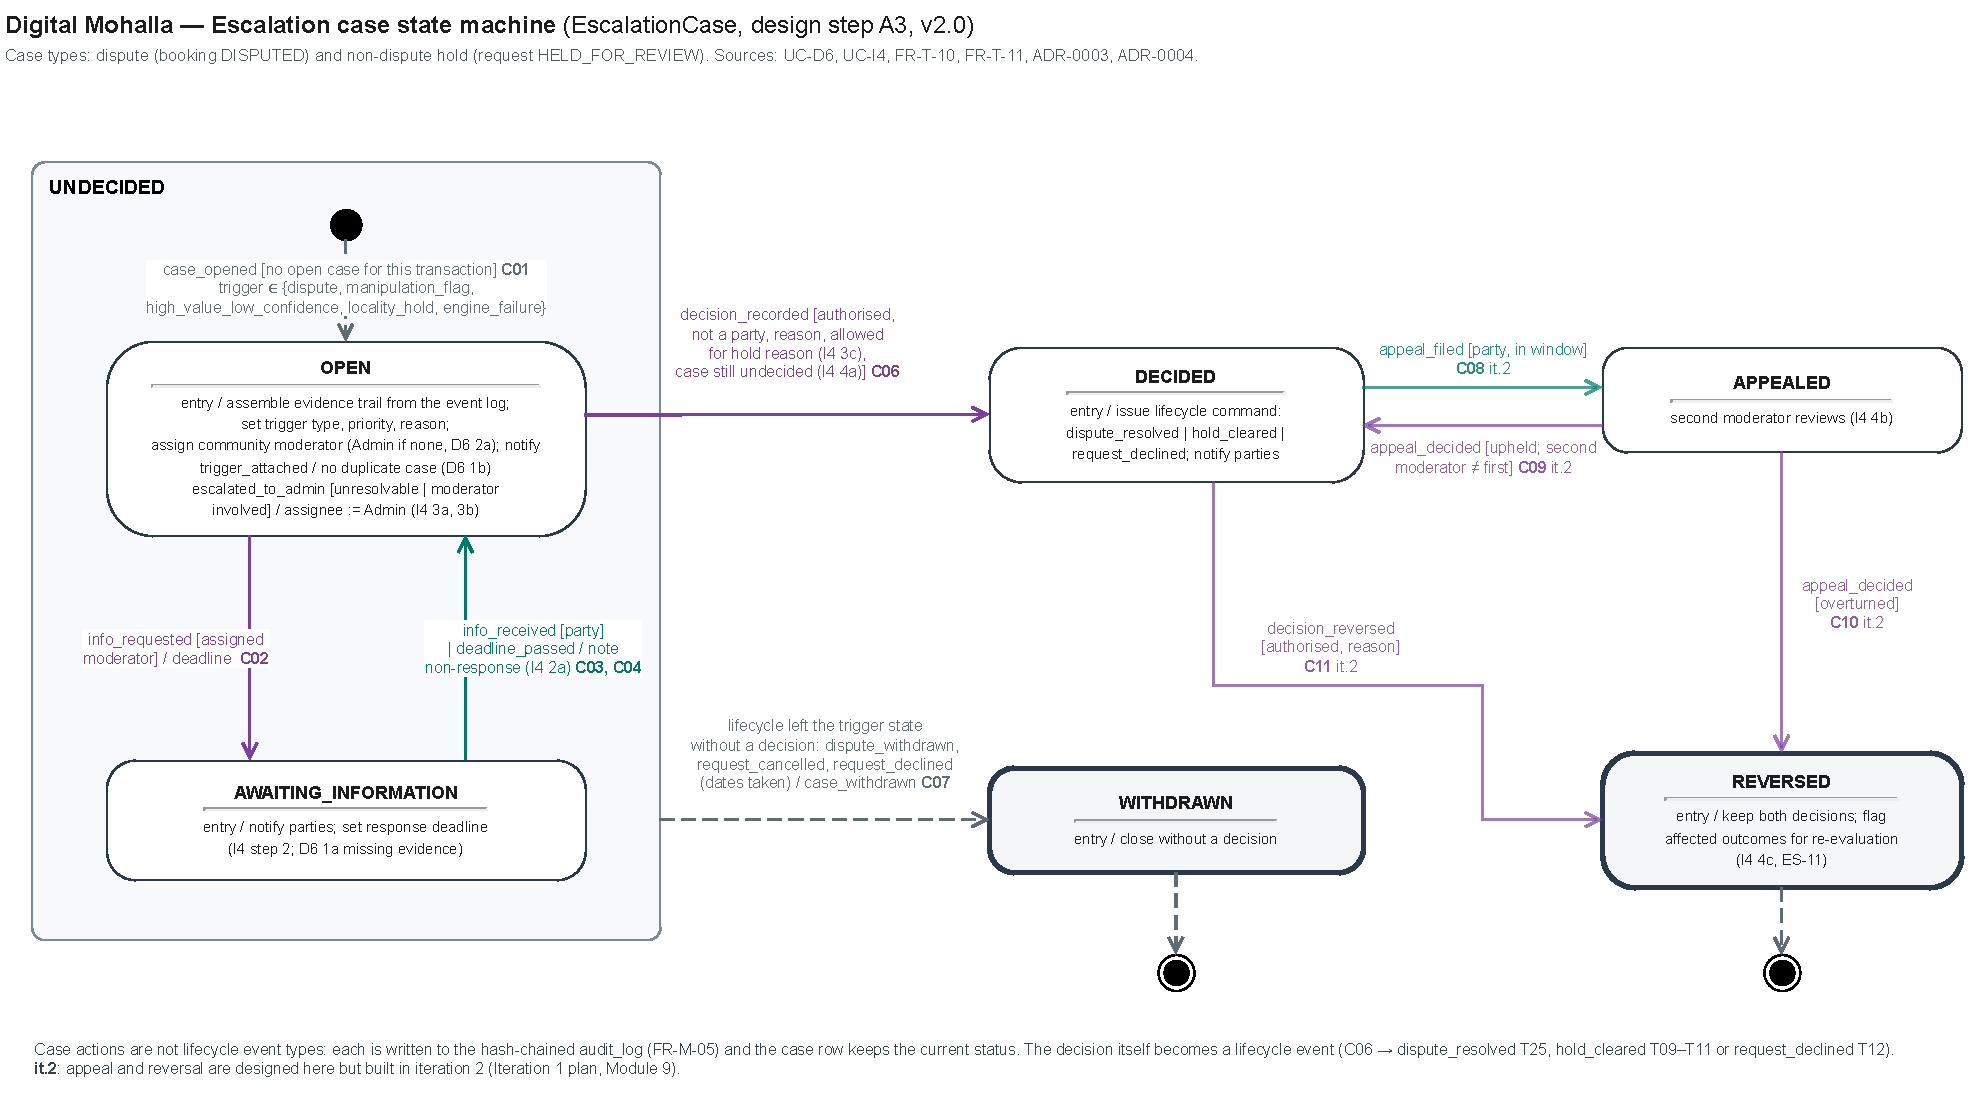
\includegraphics[width=\textwidth,height=0.80\textheight,keepaspectratio]{figures/diagrams/escalation_case_state_machine}
\caption{Escalation case state machine (UML 2.5, design step A3)}\label{fig:escalation-case-state-machine}
\drawionote{escalation_case_state_machine}{docs/design/07_state_machines/escalation_case_state_machine.drawio}
\end{figure}

\textbf{Reasoning.} A case opens for a dispute or a hold and ends either decided (with a mandatory reason) or withdrawn without a decision when the loan leaves the hold or dispute, for instance when the borrower cancels or withdraws (D9). A second dispute or hold on the same loan attaches to the open case instead of creating another (FR-T-10). A decision is stored append-only in \code{moderator_decision} and then applied as a lifecycle event in the hash-chained event log. Iteration 1 builds opening (C01), deciding (C06) and withdrawal (C07); information requests (C02--C04) and the appeal and reversal path (C08--C11) are built in Iteration 2. \textit{Serves:} FR-T-10, FR-T-11.

\subsection{Interactions}\label{sec:interactions}
\textbf{Reasoning.} The dispute freezes the loan and opens a case in the same database transaction as the \code{dispute_opened} event, so there is never a disputed loan without a case. The moderator's decision is first recorded (\code{moderator_decision}) and then applied as one lifecycle event that references it (\code{evidence_refs.decision_id}), so the decision and its effect cannot diverge. Sequence (b), handover to evidence, is in Appendix~\ref{app:additional-design-diagrams}. \textit{Serves:} FR-B-16, FR-T-10, FR-T-11. \textit{Owner:} S3.

\begin{figure}[p]
\centering
\begin{minipage}[c][0.92\textheight][c]{\textwidth}\centering
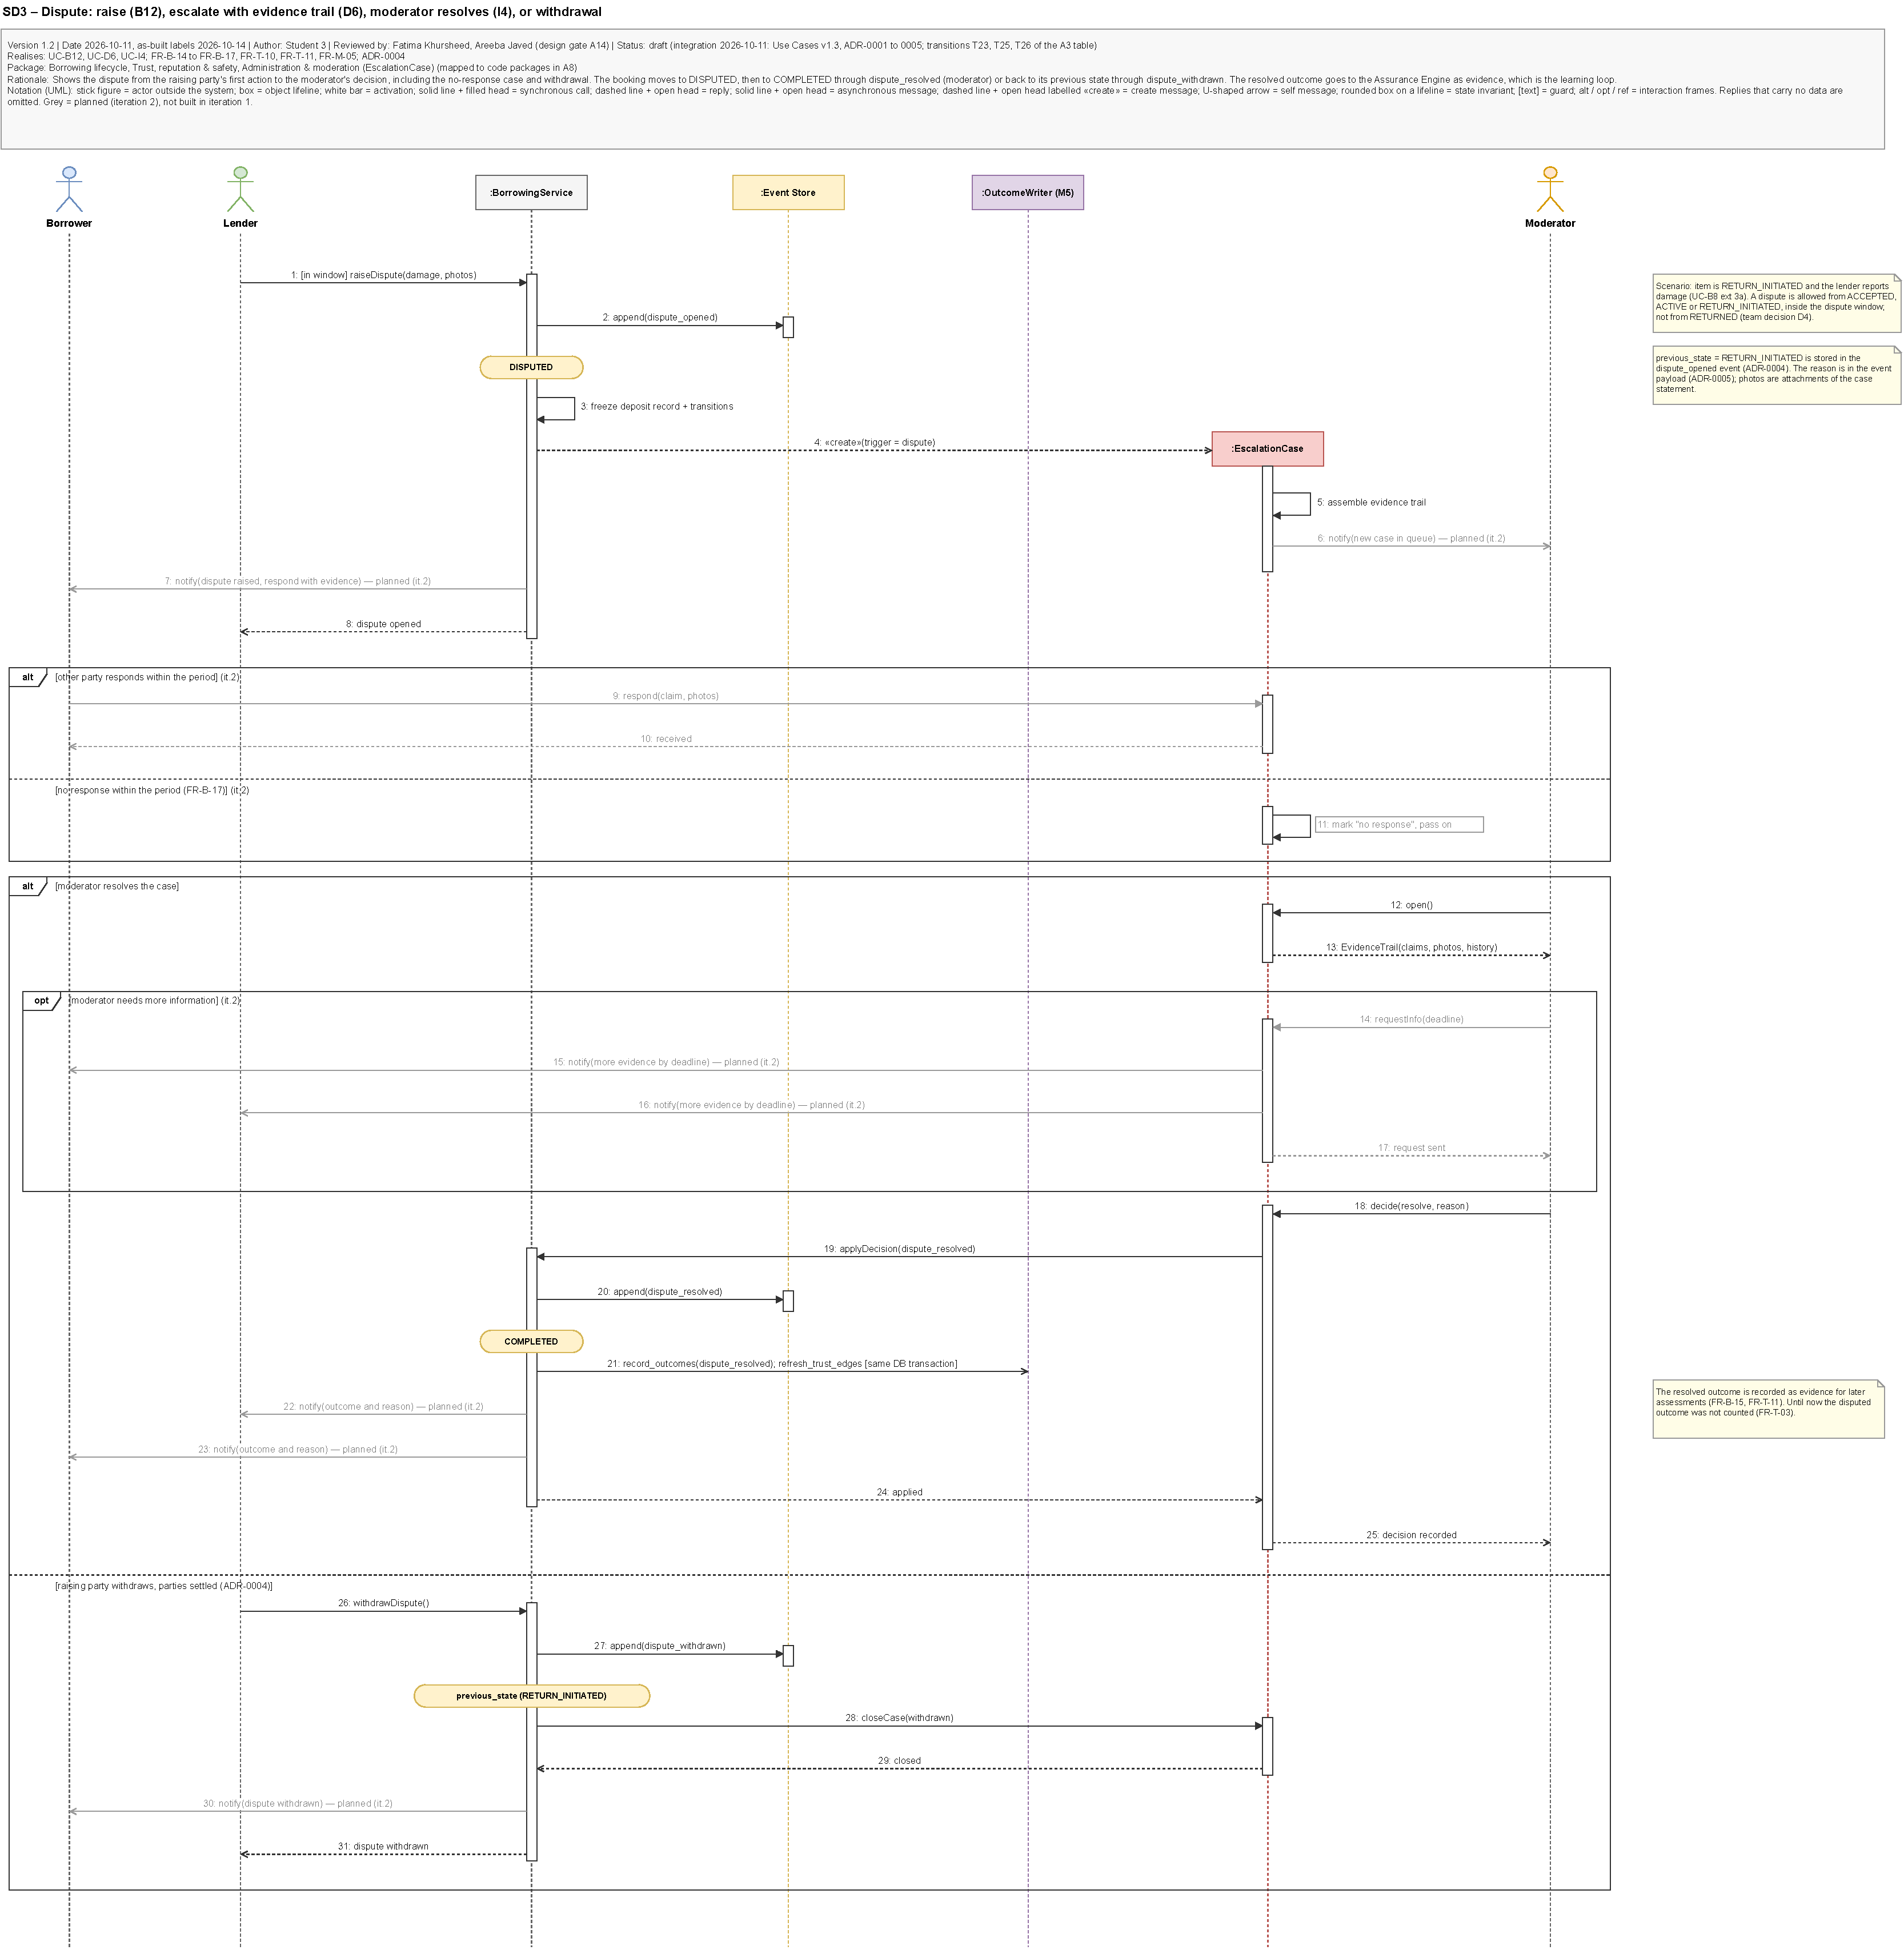
\includegraphics[width=\textwidth,height=0.80\textheight,keepaspectratio]{figures/diagrams/sequence_c_dispute}
\caption{Sequence (c): raise dispute, escalate, moderator decision (UC-B12, D6, I4)}\label{fig:sequence-c-dispute}
\drawionote{sequence_c_dispute}{docs/design/08_sequence_diagrams/sequence_c_dispute.drawio}
\end{minipage}
\end{figure}

\subsection{Data flow and privacy boundary}\label{sec:data-flow-privacy-boundary}
\begin{figure}[htbp]
\centering
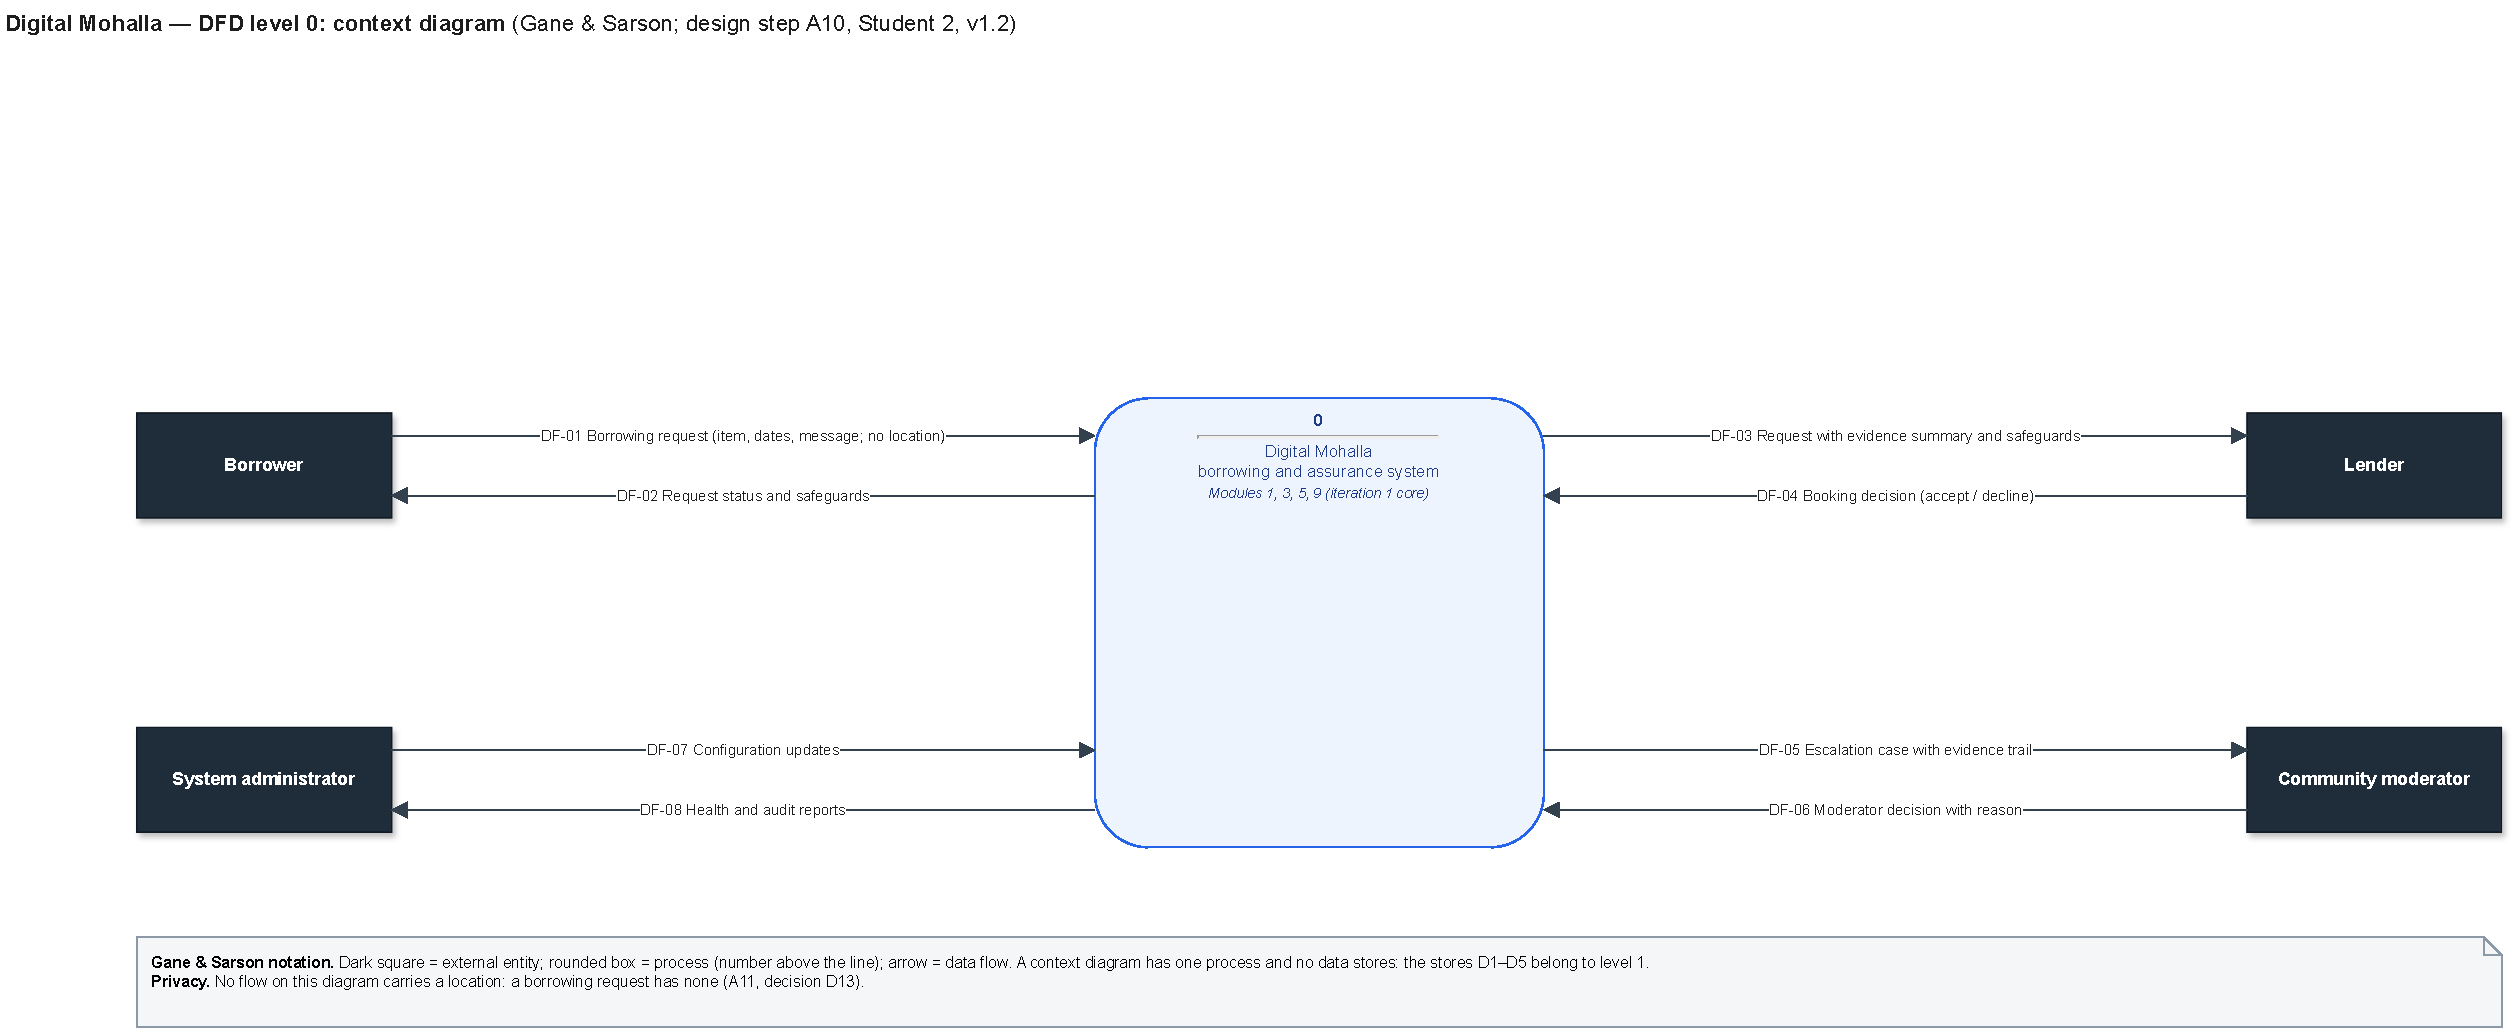
\includegraphics[width=\textwidth,height=0.80\textheight,keepaspectratio]{figures/diagrams/dfd_level0}
\caption{Assurance pipeline, DFD level 0 (context diagram; Gane and Sarson, design step A10)}\label{fig:dfd-level-0}
\drawionote{dfd_level0}{docs/design/10_dfd/dfd_assurance_pipeline_level0_level1.drawio}
\end{figure}

\textbf{Reasoning.} The context diagram shows what enters and leaves the assurance pipeline: lifecycle events and reviews in; assessments, explanations and cases out. Exact location never crosses into the pipeline: GPS is read only at membership time and reduced to a coarse result, and the request carries no location (D13). \textit{Serves:} NFR-PR-01, NFR-PR-02. \textit{Owner:} S2.

\subsection{Deployment}\label{sec:deployment}
\textbf{Reasoning and as-built deployment.} Figure~\ref{fig:deployment-diagram} shows the deployment as built; the provisional Part A design (one AWS host) is kept in Appendix~\ref{app:additional-design-diagrams} (Figure~\ref{fig:deployment-diagram-part-a}). The Part A design fixed what any target must provide: TLS termination, one API process, PostgreSQL 16 with \code{btree_gist}, migrations before start-up, a \code{/health} check and secrets outside the repository; it marked the host itself ``to be confirmed''. The confirmed target keeps every one of these properties on managed services. The API runs as a Docker container on Render (\code{digitalmohalla-api}) that applies \code{alembic upgrade head} and then starts Uvicorn; the web app is an Expo web export served by Render as a static site (\code{digitalmohalla-web}); the database is Neon PostgreSQL 16. Render deploys \code{main} only after the CI checks pass, and secrets live in Render's environment settings. \textit{Serves:} NFR-D-03, NFR-D-04, NFR-S-01.

\begin{figure}[htbp]
\centering
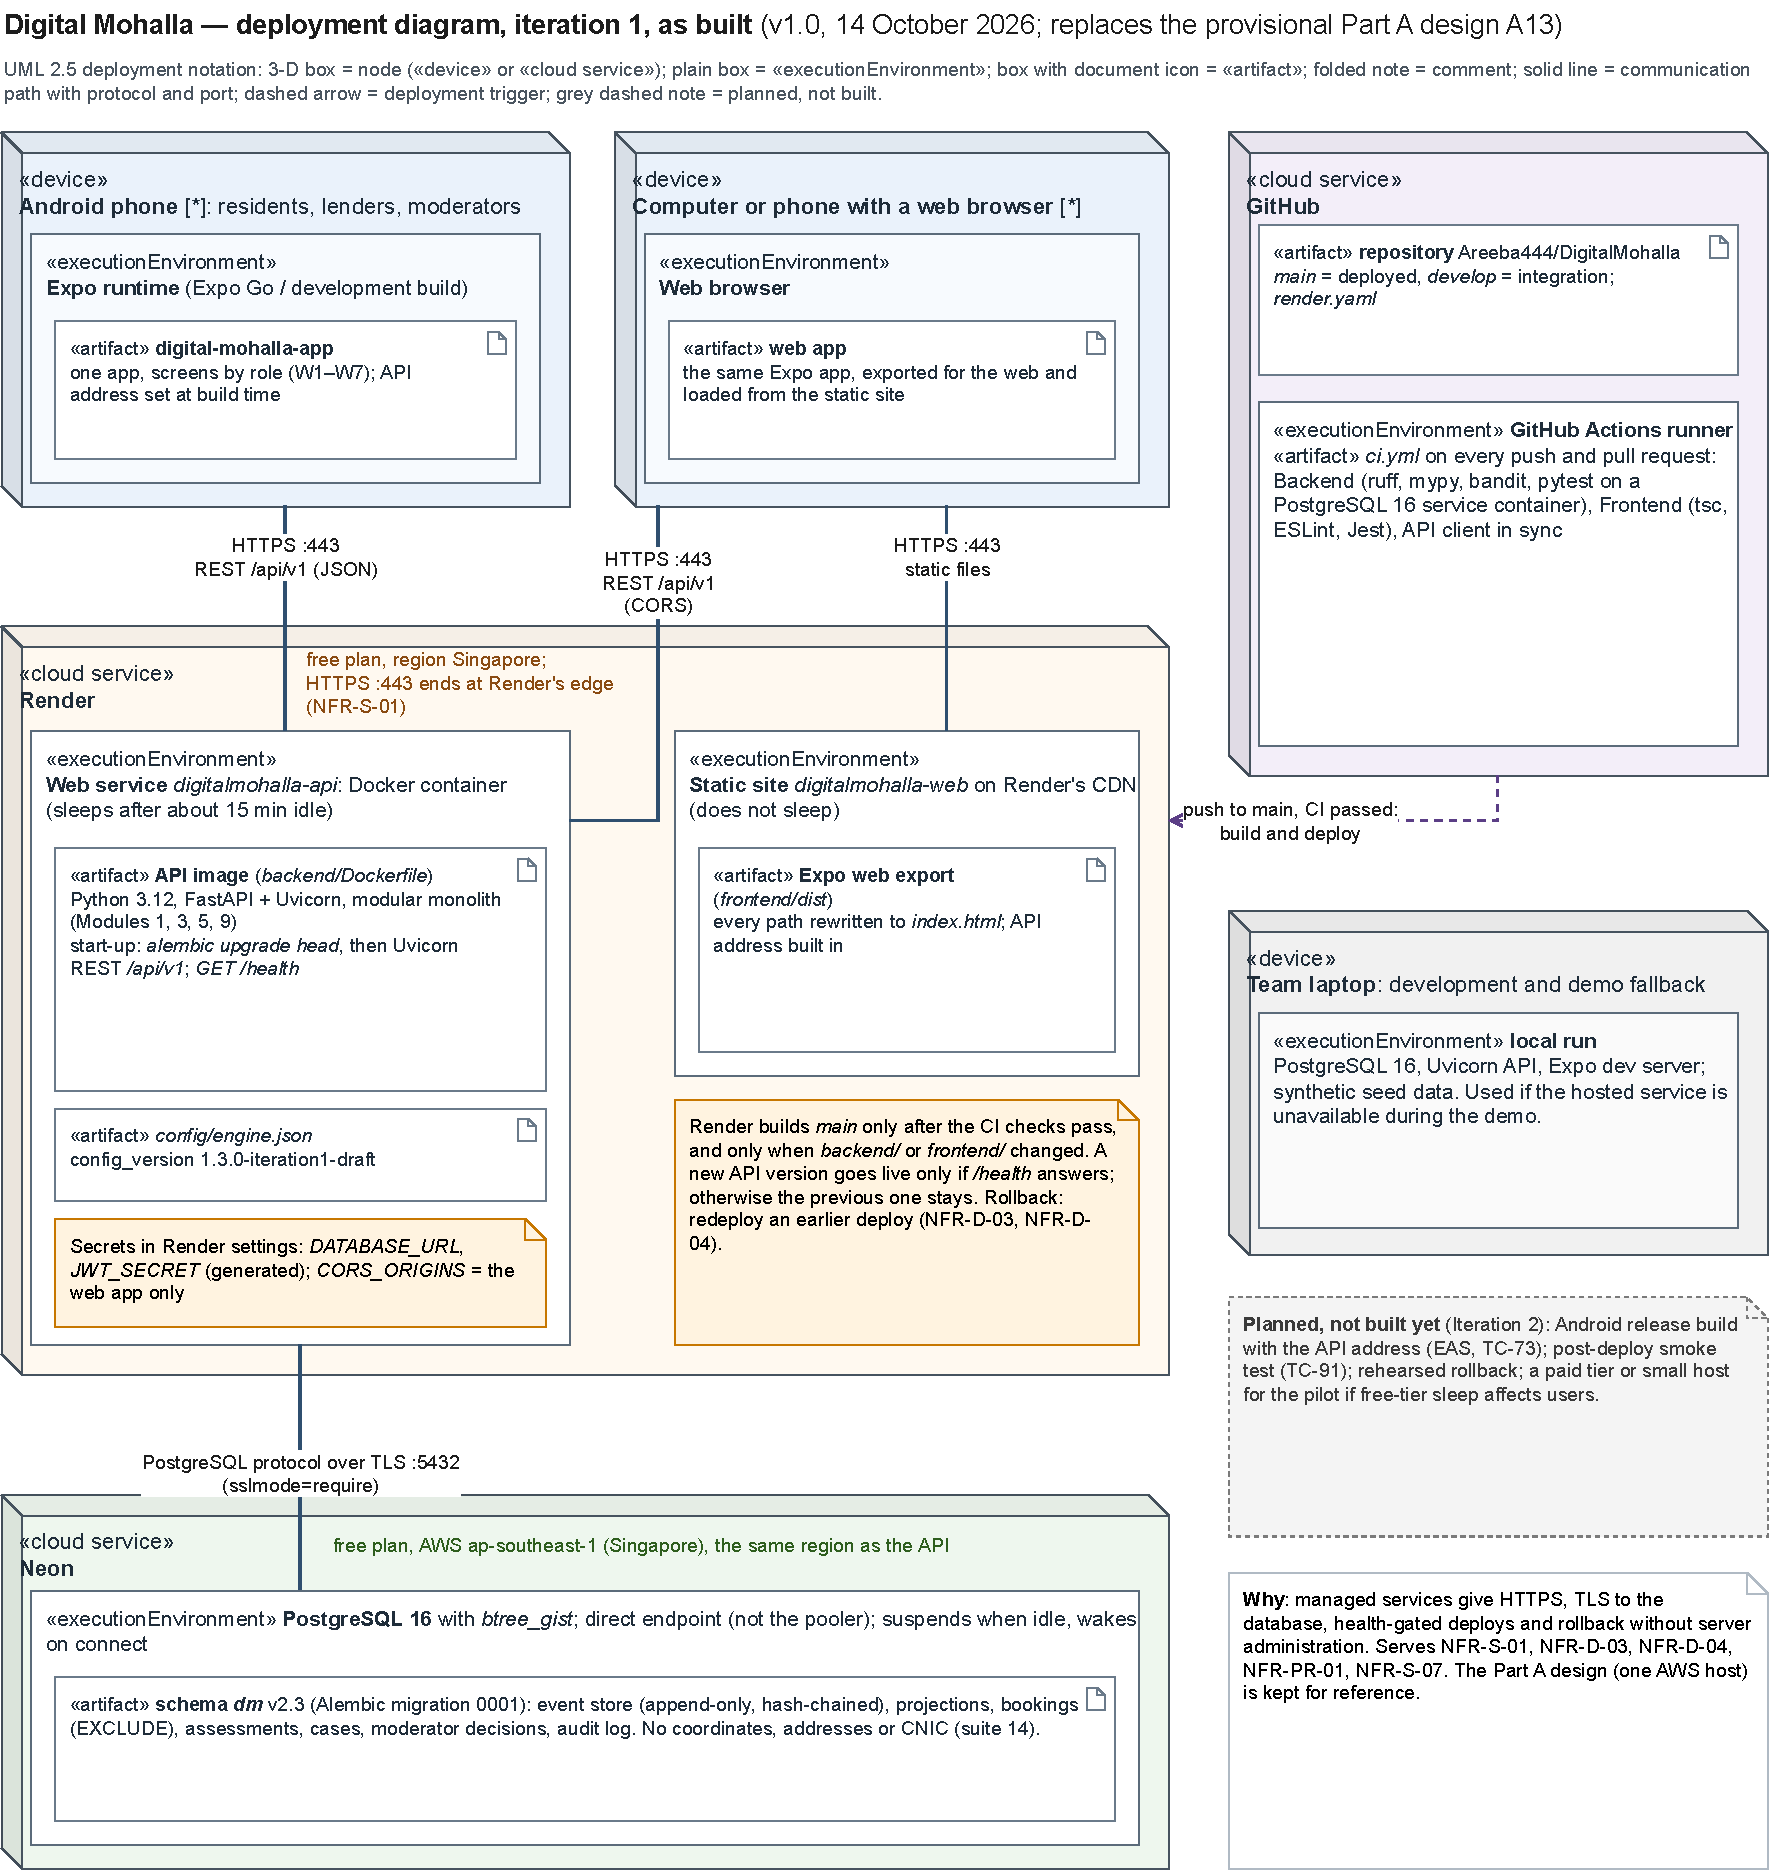
\includegraphics[width=\textwidth,height=0.80\textheight,keepaspectratio]{figures/diagrams/deployment_diagram}
\caption{Deployment diagram, Iteration 1 as built (UML 2.5): API and web app on Render, PostgreSQL 16 on Neon, deployed from \texttt{main} after CI passes}\label{fig:deployment-diagram}
\drawionote{deployment_diagram}{docs/design/04_deployment/deployment_diagram.drawio}
\end{figure}

\chapter{Iteration 1: Design and Implementation}\label{ch:iteration-1-design}
\section{Iteration Objectives}\label{sec:iteration-objectives}
\begin{enumerate}
\item A live borrowing lifecycle in which invalid transitions and double bookings cannot be stored, and every state can be rebuilt from events.
\item The assurance engine on real evidence: outcomes from closed loans, the recency-weighted posterior, indirect evidence, manipulation signals and the decision policy, with an explanation on every result.
\item The human loop: disputes, holds and moderator decisions, with a resolved dispute feeding back into evidence.
\item Evidence that the engine behaves as designed: the mid-term scenarios in CI, and $k$-hop latency and coverage measured.
\item A pipeline in which every change is checked before merge and \code{main} is deployed automatically.
\end{enumerate}

\section{Selected Use Cases / Features}\label{sec:selected-use-cases-features}
UC-B5 (request), B6 (respond), B7 (handover), B8 (return and complete), B12 (dispute), D3/4/5 (assess), D6 (escalate), I4 (resolve) and the log part of I6; minimal login (part of A2). These are the use cases on the path from a request to evidence and back, which is the shortest path that exercises the whole computing problem. Membership and locality (A3, A4) were designed but left for Iteration 2, because the lifecycle only needs the stored locality result.

\section{Design}\label{sec:design}
The iteration followed the Part A baseline in Chapter~\ref{ch:system-design}: the transition table from the state machine, the schema from the ER design, the four algorithms from the algorithm and data-structure design, and the screens from wireframes W1--W7 (Appendix~\ref{app:additional-design-diagrams}). Design questions that came up while building were settled as team decisions D10--D20 (Table~\ref{tab:team-decisions-d10-d20}) before code was merged.

\section{Implementation}\label{sec:implementation}
Work was organised as three vertical slices; each ended with a release pull request from \code{develop} to \code{main}, which triggered a deployment.

\begin{table}[!htbp]
\centering
\small
\caption{Slices and their pull requests}\label{tab:slices-their-pull-requests}
\begin{tabular}{@{}L{47pt}L{230pt}L{98pt}@{}}
\toprule
Slice & Content & Pull requests \\
\midrule
B0 & Design baseline in the repository; synthetic dataset, validator and loader; CI & \#1, \#6, \#7 \\
A & Event store, transition table, migration; engine configuration and stub engine; login and REST API; resident web app & \#2, \#3, \#4, \#5; release \#8 \\
CD & API on Render with Neon PostgreSQL; web app as a Render static site & \#17, \#20; releases \#18, \#24 \\
B & Decisions D10--D16 and test plan v1.3; outcome extraction (B1); Beta posterior and similarity (B2); trust edges (B2); $k$-hop and $k$ sweep (B3); decision policy, explanation and real engine (B4); scenario suite (B5); lender evidence screen (B6); two-theme mobile UI & \#15, \#16, \#19, \#21, \#22, \#23, \#25, \#28, \#27; releases \#29, \#30 \\
C & Manipulation checks with retaliation handling (C1); disputes (C1); moderator decisions (C2); privacy checks and fuzzing (C2); moderator app and dispute screens (C3) & \#31--\#35; release \#36 \\
\bottomrule
\end{tabular}
\end{table}
\section{Completed Features / Module}\label{sec:completed-features-module}
\begin{table}[H]
\centering
\small
\caption{Completed features}\label{tab:completed-features}
\begin{tabular}{@{}L{98pt}L{209pt}L{68pt}@{}}
\toprule
Feature & What works & Module, owner \\
\midrule
Event store and lifecycle & 14 states, 21 event types; append-only, hash-chained events; replay in Python and SQL; invalid transitions refused twice and audited & 3, S1 \\
Request to completion & Request, locality read, assessment, accept (overlapping requests declined), decline, cancel, handover checklist and confirmation with deposit record, return, on-time or late close & 3, S1 \\
Double-booking guard & Exclusion constraint; exactly one of N simultaneous acceptances commits & 3, S1 \\
Outcome extraction & Confirmed outcomes per role and metric on close; disputed outcomes excluded until resolved & 5, S2 \\
Beta posterior & Recency and similarity weights; 90\% interval; effective evidence & 5, S2 \\
Trust edges and $k$-hop & Edge weights from verified outcomes; bounded search with decay, path diversity, noisy-OR and cap; paths shown to the lender & 5, S1 \\
Manipulation checks & S1 partner clustering, S4 review similarity, corroboration rule, retaliation set-aside & 5, S2 \\
Decision policy and explanation & Rules R1--R9, safeguards, plain-language explanation; engine timeout or failure holds & 5, S2 \\
Disputes & Raise (freezes the loan, opens a case), view, withdraw (restores the previous state) & 3/9, S3 \\
Moderator decisions & Queue of disputes and holds for the moderator's community; decisions with a mandatory reason; resolved outcome becomes evidence & 9, S3 \\
Privacy checks & Response-model scan, whole-loan key and value checks, log and audit scan, strict request bodies, fuzzing & cross-cutting, S1 \\
Apps & Resident app (browse, request, lender evidence, handover, return, dispute) and moderator app (queue, case adjudication), two themes & apps, S3 \\
Synthetic data and scenarios & Seeded generator (mini, standard, scale tiers), validator, loader; scenario suite in CI & 10, S3 \\
CI/CD & Three CI jobs on every push and pull request; automatic deploy of \code{main} after CI & S1 (CI), Render deploys \\
\bottomrule
\end{tabular}
\end{table}
\section{Technical Implementation Details}\label{sec:technical-implementation-details}
\subsection{Code organisation}\label{sec:code-organisation}
The backend follows the layout in the tech-stack document: \code{app/api} (routes, schemas, dependencies), \code{app/domain} (\code{lifecycle}, \code|assurance/{estimation, indirect, detection,| \code|policy}|, \code{moderation}, \code{accounts}), \code{app/infra} (\code{db}, \code{eventstore}) and \code{app/config}. The domain packages contain no input/output. The backend application is 4,383 lines of Python in 33 files, and its tests are 5,092 lines; the frontend is about 4,200 lines of TypeScript excluding the generated client.

\begingroup\small
\begin{longtable}{@{}L{149pt}L{230pt}@{}}
\caption{Key files, classes and functions}\label{tab:key-files-classes-functions}\\
\toprule
File & Main elements \\
\midrule
\endfirsthead
\toprule
File & Main elements \\
\midrule
\endhead
\bottomrule
\endlastfoot
\code{domain/lifecycle/service.py} & \code{BorrowingService}: \code{create_request}, \code{accept}, \code{decline_overlapping}, \code{confirm_handover}, \code{confirm_return}, \code{raise_dispute}, \code{withdraw_dispute}, \code{decide}, \code{moderation_queue}; engine call with timeout \\
\code{domain/lifecycle/transition_table.py} & \code{TransitionTable.load}, \code{lookup}, \code{is_valid}, \code{next_state} (from \code{transition_table.csv}) \\
\code{domain/lifecycle/aggregate.py} & \code{BorrowingTransaction.apply}, \code{replay} (gap, order and previous-state checks) \\
\code{domain/lifecycle/ports.py} & \code{IAssess}, \code{LifecycleStore}, \code{AuditLog}; \code{AssessmentRequest}, \code{AssessmentResult} \\
\code{infra/eventstore/store.py}, \code{postgres.py} & \code{create_request}, \code{append}, \code{load_stream}, \code{replay_state}, \code{verify_chain}; database error mapping; \code{PostgresAuditLog} \\
\code{domain/assurance/engine.py} & \code{AssuranceEngine.assess}; \code{EvidenceSource} protocol \\
\code{assurance/estimation/posterior.py}, \code{similarity.py}, \code{outcomes.py} & \code{recency_weight}, \code{credible_interval}, \code{estimate}; similarity (D17); outcome rules (D11) \\
\code{assurance/indirect/khop.py}, \code{edges.py} & \code{find_paths}, \code{path_strength}, \code{indirect_trust}; \code{edge_weight}, \code{build_edges} \\
\code{assurance/detection/manipulation.py} & \code{partner_clustering}, \code{review_similarity}, \code{max_cosine}, retaliation flags, \code{combine} \\
\code{assurance/policy/decision.py}, \code{explanation.py} & \code{RULES}, \code{decide}, \code{safeguards_for}; \code{build_explanation} \\
\code{domain/moderation/decisions.py} & \code{plan} (which event a decision produces), \code{InvalidDecision} \\
\code{api/routes.py}, \code{schemas.py} & 21 API endpoints (plus \code{/health} in \code{main.py}); \code{StrictIn} request base (unknown fields and NUL characters refused) \\
\code{config/engine.json} & Versioned parameters (\code{1.3.0-iteration1-draft}), one section per algorithm \\
\code{frontend/src/app/(resident)}, \code{(moderator)} & Expo Router screens; \code{src/api} generated typed client; \code{AssurancePanel} \\
\end{longtable}
\endgroup
\subsection{Configuration}\label{sec:configuration}
Every tunable value lives in \code{backend/config/engine.json}, marked \code{initial_hypothesis_unvalidated}, with a sensitivity range for the FYP-2 study. The loader refuses a file with a missing or out-of-range parameter (TC-74), and every stored assessment records the version it used. The version has moved from \code{1.0.0} (initial parameter set) and \code{1.1.0} (integration: S4 active, R6\_SPARSE, ADR-0007 and ADR-0008), both in Part A, to \code{1.2.0} (similarity, D17) and \code{1.3.0} (manipulation checks, D18, D19), each change recorded in the file's changelog.

\subsection{Coding conventions and static analysis}\label{sec:coding-conventions-static-analysis}
Python follows ruff's lint rules and formatter (line length 100); the domain packages pass \code{mypy}; \code{bandit} scans for insecure patterns and \code{pip-audit} for vulnerable dependencies. TypeScript is checked with \code{tsc} and ESLint, and formatted with Prettier. Every module that contains maths or a non-obvious rule starts with a plain-language note explaining what it does and why it was chosen over the alternative, so that any member can explain it.

\section{Algorithms and Technical Decisions}\label{sec:algorithms-technical-decisions}
The four algorithms below are implemented as specified in the Part A algorithm and data-structure design. All parameter values quoted are those of the current configuration, version \code{1.3.0-iteration1-draft}.

\subsection{Algorithm 1: recency-weighted Beta posterior (S2)}\label{sec:algorithm-1-recency-weighted-beta}
Each confirmed outcome $i$ of the borrower in the borrower role is a success ($y_i = 1$) or a failure ($y_i = 0$) for one metric. An outcome $d_i$ days old with similarity $\sigma_i$ to the request has weight
\[
w_i = 2^{-d_i/h}\,\max(\sigma_{\min}, \sigma_i), \qquad h = 180 \text{ days},\ \sigma_{\min} = 0.5,
\]
where $\sigma_i = 0.4\,c_{\mathrm{band}} + 0.4\,[\text{same category}] + 0.2\,\frac{\text{shorter duration}}{\text{longer duration}}$ and $c_{\mathrm{band}}$ is 1, 0.5 or 0 for the same, an adjacent or a distant value band (D17). With $s = \sum w_i y_i$ and $f = \sum w_i (1 - y_i)$ the posterior is $\mathrm{Beta}(1+s,\,1+f)$; the engine reports its mean, the 5\% and 95\% quantiles (the 90\% credible interval) and the effective evidence $n_{\mathrm{eff}} = s + f$. With no history this is $\mathrm{Beta}(1,1)$: mean 0.5, interval $[0.05, 0.95]$, which the policy reports as INSUFFICIENT\_EVIDENCE, not as a low value. \textit{Check values tested}: weights 0.962 and 0.25 at 10 and 360 days; 18 successes and 2 failures give $\mathrm{Beta}(19,3)$. \textit{Complexity}: $O(n)$ time for $n$ outcomes, $O(1)$ extra space. \textit{Why}: a conjugate posterior gives an honest interval from very few observations \cite{josang2002beta}, and the half-life lets old behaviour fade without being forgotten.

\subsection{Algorithm 2: bounded $k$-hop indirect evidence (S1)}\label{sec:algorithm-2-bounded-hop-indirect}
Trust edges are derived only from verified outcomes (ADR-0006): the weight of edge $(a,b)$ is the posterior mean of $a$'s verified outcomes with $b$. For a lender $u$ and borrower $v$:

\begin{enumerate}
\item Find simple paths from $u$ to $v$ of at most $k = 3$ edges (depth-first, no repeated node, so cycles are safe).
\item Score a path $P$ with $h$ edges as $q(P) = \gamma^{h-1} \prod_{e \in P} w_e$, with $\gamma = 0.7$ (the first hop is not penalised).
\item Keep only the strongest path per first-hop neighbour; paths through the same neighbour are not independent evidence.
\item Combine with noisy-OR: $I = 1 - \prod_{P} (1 - q(P))$.
\item Reliability $\rho = \min\bigl(0.6,\ \min(1, |P|/3) \cdot \min(1, |F|/2) \cdot I\bigr)$, where $|F|$ is the number of distinct first hops.
\item Indirect estimate $t_{\mathrm{ind}} = b + \rho\,(t_v - b)$, with population baseline $b = 0.5$.
\end{enumerate}

The cap $\rho \leq 0.6$ keeps indirect evidence below direct evidence, and the policy never lets $\rho$ alone produce SUFFICIENT\_EVIDENCE. \textit{Complexity}: $O\bigl(\sum_{i=1}^{k} \Delta^{i}\bigr)$ for maximum out-degree $\Delta$. On the hand-worked 8-node graph the code reproduces the designed values ($I = 0.7164$, $\rho = 0.6$ capped; $\rho = 0, 0.424, 0.600, 0.600$ for $k = 1..4$). \textit{Why}: trust that weakens with distance follows Golbeck \cite{golbeck2005}; the cap, the path-diversity rule and the bounded $k$ are the project's adaptations for small, dense neighbourhood graphs.

\textbf{$k$ sweep.} Table~\ref{tab:sweep-scale-tier-synthetic} reports latency and coverage for $k = 1$ to 4 on the synthetic \textit{scale} tier (2,026 users, 5,987 edges, seed 20261001), one search per (lender, borrower) pair of 2,000 loans. $k = 3$ finds a path for 93.2\% of pairs at 4.5 ms (P95); $k = 4$ adds one percentage point of coverage at 3.5 times the P95 latency and 7 times the maximum, so $k = 3$ is kept. The sweep was measured with configuration 1.2.0; version 1.3.0 changed only manipulation-detection parameters, so the $k$-hop results still apply. \textit{Caveat:} the pairs are existing loans, so a direct edge between lender and borrower usually exists already, and the $k = 1$ coverage (80.3\%) includes the assessed loan's own edge. This overstates coverage for genuinely new pairs; the FYP-2 evaluation uses time-ordered held-out pairs instead.

\begin{table}[!htbp]
\centering
\caption{$k$ sweep on the scale tier (SYNTHETIC data, config 1.2.0)}\label{tab:sweep-scale-tier-synthetic}
\begin{tabular}{@{}crrrrr@{}}
\toprule
$k$ & P50 (ms) & P95 (ms) & max (ms) & coverage & pairs, $\rho \geq \rho_{\mathrm{sup}}$ \\
\midrule
1 & 0.025 & 0.080 & 3.871 & 80.3\% & 0 \\
2 & 0.087 & 0.709 & 15.543 & 88.9\% & 946 \\
3 & 0.439 & 4.519 & 28.488 & 93.2\% & 1,346 \\
4 & 2.279 & 15.915 & 207.045 & 94.2\% & 1,435 \\
\bottomrule
\end{tabular}
\par\vspace{0.3em}{\small Windows AMD64, Python 3.12.11, commit \code{f7afd92}; raw output in \code{docs/design/14_testing/results/}.\par}
\end{table}

\subsection{Algorithm 3: manipulation-risk scoring (S2)}\label{sec:algorithm-3-manipulation-risk-scoring}
Manipulation risk is a separate 0--100 dimension, never averaged with trust. Iteration 1 computes two signals and one check over a 90-day window:

\begin{itemize}
\item \textbf{S1, partner clustering (D18).} Take the borrower's review partners (at least 3). Let $r$ be the share of pairs of partners who reviewed each other in both directions; $S_1 = \mathrm{clip}\bigl((r - 0.3)/0.6\bigr)$. A ring of accounts fills almost every pair; an ordinary borrower's lenders rarely review one another. The simpler ``A rated B and B rated A'' rule was rejected because every loan produces two reviews: on the standard tier it flagged 6 of 8 ordinary members; partner clustering flags 0 of 9.
\item \textbf{S4, similar review texts.} The reviews the borrower received, as character 3-grams weighted by TF-IDF; the highest cosine similarity $c$ between two of them gives $S_4 = \mathrm{clip}\bigl((c - 0.7)/0.25\bigr)$.
\item \textbf{Retaliation check (D19).} A low review (lowest rating $\leq 2$) posted within 14 days after the subject complained about its author, about a loan whose return was confirmed, is set aside: left out of S1 and S4, reported, and explained to the lender in neutral words.
\end{itemize}

The score is the weighted mean over the available signals, $\text{score} = 100 \cdot \sum_i w_i s_i \big/ \sum_i w_i$ (with $w_{S1} = 0.3$, $w_{S4} = 0.2$; a signal without enough data is left out of both sums), banded into levels 1 to 4 at 20, 40 and 60. Level 4 additionally requires two signals $\geq 0.5$ (ADR-0007); otherwise the result is level 3. A legitimate family group therefore stays at level 3 (TC-38): extra verification, no hold. \textit{Complexity}: S1 $O(p^2)$ for $p$ partners; S4 $O(m^2 L)$ for $m$ reviews of length $L$. \textit{Why}: collusion shows as groups that rate one another \cite{mukherjee2012,hooi2016}, while two-sided reviews are reciprocal by nature \cite{bolton2013,fradkin2021}. \textit{Known limit}: a ring that also trades with outsiders lowers its own density (camouflage).

\subsection{Algorithm 4: decision policy (S2)}\label{sec:algorithm-4-decision-policy-s2}
The first rule whose condition holds decides (Table~\ref{tab:decision-rules-order-algorithm}). Thresholds (D12): $\tau_\mu = 0.75$, $\tau_L = 0.60$, $n_{\min} = 3$, $\rho_{\mathrm{sup}} = 0.3$.

\begin{longtable}{@{}L{39pt}L{150pt}L{98pt}L{76pt}@{}}
\caption{Decision rules in order (Algorithm 4)}\label{tab:decision-rules-order-algorithm}\\
\toprule
Rule & Condition & State & Lifecycle \\
\midrule
\endfirsthead
\toprule
Rule & Condition & State & Lifecycle \\
\midrule
\endhead
\bottomrule
\endlastfoot
R1 & An open dispute involves the borrower & ACTIVE\_DISPUTE & ASSESSED \\
R2 & Manipulation level 4 (corroborated) & REVIEW\_RECOMMENDED & HELD (\code{manipulation_risk}) \\
R3 & No verified history and $\rho < \rho_{\mathrm{sup}}$ & INSUFFICIENT\_EVIDENCE & ASSESSED \\
R4 & High value and (similarity $< 0.5$ or lower bound $< \tau_L$) & REVIEW\_RECOMMENDED & HELD (\code{high_value_low_confidence}) \\
R5 & Manipulation level 3 & REVIEW\_RECOMMENDED & ASSESSED \\
R6\_DISPUTE & A resolved dispute in the last 12 months & REVIEW\_RECOMMENDED & ASSESSED \\
R6\_SPARSE & $n_{\mathrm{eff}} < n_{\min}$ and $\rho < \rho_{\mathrm{sup}}$ & INSUFFICIENT\_EVIDENCE & ASSESSED \\
R7 & Mean $\geq \tau_\mu$, lower bound $\geq \tau_L$, $n_{\mathrm{eff}} \geq n_{\min}$, level 1, standard value, verified & SUFFICIENT\_EVIDENCE & ASSESSED \\
R8 & As R7 but level 2, or medium or high value & SUFFICIENT\_EVIDENCE with safeguards & ASSESSED \\
R9 & Anything else (e.g. sparse but supported by community paths) & REVIEW\_RECOMMENDED & ASSESSED \\
\end{longtable}
Because R7 and R8 need $n_{\mathrm{eff}} \geq 3$ from the borrower's own outcomes, indirect evidence alone can never yield SUFFICIENT\_EVIDENCE (property-tested, TC-34). Each rule maps to a policy decision and a set of safeguards (deposit record, handover photos and checklist, fixed return date, verification), and the explanation names the rule, the interval, the effective evidence, the community paths and the signals. The database refuses an assessment row whose rule, state, decision and hold reason disagree (\code{assessment_rule_ck}). \textit{Complexity}: $O(1)$ given the inputs; a whole assessment is $O(n) + O(\Delta^k) + O(p^2 + m^2 L)$.

\subsection{Other technical decisions}\label{sec:other-technical-decisions}
\begin{itemize}
\item \textbf{Engine timeout.} The lifecycle calls the engine in a worker with a 2,000 ms timeout from the configuration; a timeout or exception holds the request with \code{engine_failure} and stores no assurance state.
\item \textbf{Moderator decisions.} \code{plan()} turns a decision into exactly one lifecycle event (\code{dispute_resolved}, \code{hold_cleared} or \code{request_declined}) according to the hold reason, and refuses invalid combinations, such as safeguards on an engine-failure hold.
\item \textbf{Strict request bodies.} Every request schema refuses unknown fields and NUL characters, so a client cannot inject \code{actor_id}, \code{authorisation} or \code{new_state}.
\end{itemize}

\section{Tools, Frameworks and Technologies}\label{sec:tools-frameworks-technologies}
\begin{table}[H]
\centering
\caption{Technology stack}\label{tab:technology-stack}
\begin{tabular}{@{}L{90pt}L{289pt}@{}}
\toprule
Layer & Choice \\
\midrule
Backend & Python 3.12, FastAPI, Pydantic, SQLAlchemy 2 (synchronous) with psycopg 3, Alembic, NumPy and SciPy (Beta quantiles), argon2 password hashing, JWT tokens, managed with uv \\
Database & PostgreSQL 16 with \code{btree_gist}; triggers and constraints for the event store \\
Frontend & React Native with Expo SDK 57, Expo Router, React Native Paper, TanStack Query, \code{openapi-fetch} with a client generated by \code{openapi-typescript}; Android and web \\
Testing & pytest, Hypothesis (property-based tests and fuzzing), Jest with React Native Testing Library \\
Quality & ruff, mypy, bandit, pip-audit, ESLint, tsc, Prettier, npm audit, Dependabot \\
CI/CD & GitHub Actions; Render (Docker web service and static site); Neon PostgreSQL \\
\bottomrule
\end{tabular}
\end{table}
\section{Demonstration Evidence}\label{sec:demonstration-evidence}
\begin{itemize}
\item \textbf{Live system.} API: \code{https://digitalmohalla-api.onrender.com} (\code{/health} returns 200); web app: \code{https://digitalmohalla-web.onrender.com}. Both returned HTTP 200 on 14 October 2026. Demo accounts and data are synthetic.
\item \textbf{Repository.} \code{https://github.com/Areeba444/DigitalMohalla}: 36 pull requests (30 merged), CI history, release pull requests to \code{main}.
\item \textbf{Screens.} The built screens follow wireframes W1--W7 (Appendix~\ref{app:additional-design-diagrams}): the lender's request view with the assurance panel (W1), decision (W2), handover (W3), return (W4), dispute form (W5), moderator queue (W6) and case adjudication (W7).
\item \textbf{Demo script.} (1) A newcomer's request gives INSUFFICIENT\_EVIDENCE with a wide interval and safeguards; (2) a borrower known only through neighbours (ES-13) shows the community paths; (3) an established borrower gives SUFFICIENT\_EVIDENCE; (4) accept, hand over, return with damage, dispute; (5) the next request shows ACTIVE\_DISPUTE; (6) the moderator decides with a reason and the loan completes; plus an invalid transition rejected, two simultaneous acceptances, the colluding scenario held for review, and the CI pipeline.
\end{itemize}

\section{Iteration Outcome}\label{sec:iteration-outcome}
Iteration 1 met its objectives: all three slices are merged and deployed, the mid-term scenario target is met (7 of 7), and 623 backend and 29 frontend tests pass. What is left from the plan is listed in Section~\ref{sec:delays-deviations-recovery-plan}; none of it blocks the demo story.

\chapter{Testing and Early Validation}\label{ch:testing-early-validation}
Testing follows \textit{Test Plan v1.3} (\code{docs/design/14_testing/Test_Plan.md}): 19 suites, test cases written as input / expected / actual, and traceability to requirements. All test data is synthetic.

\section{Testing Strategy}\label{sec:testing-strategy}
\begin{itemize}
\item \textbf{Test the invariants where they are enforced.} Rules that must never break (valid transitions, no overlapping bookings, append-only events, \code{config_version} on every assessment) are enforced in PostgreSQL, so they are tested against a real PostgreSQL 16 database, not a mock.
\item \textbf{Test the maths against worked numbers.} Every algorithm was worked by hand in Part A (an 8-node graph, thirteen scenario fixtures, check values such as Beta(19,3)); the code must reproduce those numbers. The $k$-hop search is also cross-checked against NetworkX.
\item \textbf{Test properties, not only examples.} Hypothesis generates inputs for the posterior (the mean always lies inside its interval; another success never lowers the mean), the policy (indirect evidence alone is never SUFFICIENT), the $k$-hop search and the API (fuzzing).
\item \textbf{Test behaviour end to end.} The scenario suite drives the real engine through the real lifecycle on a synthetic neighbourhood and checks the state, the rule and the explanation.
\item \textbf{Deterministic.} Fixed seeds (dataset seed 20261001), no network calls, and the same tests in CI as on a laptop.
\item \textbf{Gate every change.} A pull request cannot be merged until the three CI jobs pass (NFR-D-04).
\end{itemize}

\section{Test Levels and Techniques}\label{sec:test-levels-techniques}
\begin{table}[H]
\centering
\caption{Test levels}\label{tab:test-levels}
\begin{tabular}{@{}L{68pt}L{39pt}L{268pt}@{}}
\toprule
Level & Tests & What is tested \\
\midrule
Unit (backend) & 477 & Transition table (all 294 pairs), aggregate and replay, posterior, similarity, outcome rules, trust edges, $k$-hop, manipulation signals, decision policy, explanation, moderation rules, configuration, generator \\
Integration (backend) & 102 & Event store and triggers, lifecycle service, concurrency, authorisation, disputes, moderation, outcome and trust-edge feeds, privacy, API, fuzzing, engine on the synthetic dataset \\
Scenario / acceptance & 44 & ES scenarios on the fixtures and end to end; lender evidence API \\
Frontend component & 29 & Screens W1, W5, W6 and W7 rendered with React Native Testing Library against a mocked API; formatting and moderation helper functions \\
Total & 652 & 623 backend, 29 frontend \\
\bottomrule
\end{tabular}
\end{table}
Techniques: state-transition testing (the full matrix), decision-table testing (rules R1--R9, moderator decisions), boundary values (value bands at 5,000/5,001 and 15,000/15,001 PKR; 10 and 360 days of age), concurrency testing (parallel acceptances behind a barrier), fault injection (engine timeout and exception), property-based testing, oracle testing (worked examples, NetworkX), fuzzing (API bodies), and static analysis (ruff, mypy, bandit, ESLint, tsc).

\section{Test Cases}\label{sec:test-cases}
Table~\ref{tab:representative-test-cases-input} shows representative test cases, one or more per suite; Appendix~\ref{app:detailed-test-cases} lists all implemented ones.

\begingroup
\begin{longtable}{@{}L{26pt}L{111pt}L{158pt}L{64pt}@{}}
\caption{Representative test cases (input / expected / actual)}\label{tab:representative-test-cases-input}\\
\toprule
TC & Input & Expected & Actual \\
\midrule
\endfirsthead
\toprule
TC & Input & Expected & Actual \\
\midrule
\endhead
\bottomrule
\endlastfoot
TC-01 & Each of the 294 state--event pairs & 31 valid pairs accepted; 263 refused & Pass (297 tests) \\
TC-02 & COMPLETED loan; lender sends accept & 409 ``invalid transition''; audit entry & Pass \\
TC-05 & RETURNED loan; dispute & Refused (decision D4) & Pass \\
TC-07 & Happy path, 8 events & Replay equals the stored state & Pass \\
TC-08 & 5 parallel acceptances, overlapping dates, 3 rounds & Exactly one ACCEPTED per round; others DECLINED ``dates taken'' & Pass \\
TC-13/14 & UPDATE or DELETE on events; an edited event & Refused; tampering detected by \code{verify_event_chain()} & Pass \\
TC-20 & No outcomes & Beta(1,1), mean 0.5, 90\% CI [0.05, 0.95] & Pass \\
TC-22 & Ages 10 and 360 days, $h = 180$ & Weights 0.962 and 0.25 & Pass \\
TC-25 & 8-node hand-worked graph, $k=3$ & 3 paths ($q$ = 0.54, 0.2195, 0.21), $I = 0.7164$, $\rho = 0.6$ & Pass \\
TC-28 & Graph with a cycle and a self-loop & Search terminates; no repeated node & Pass \\
TC-34 & Hypothesis: only indirect evidence is strong & Never SUFFICIENT\_EVIDENCE & Pass \\
TC-36 & Engine stub sleeps past the timeout & HELD\_FOR\_REVIEW (\code{engine_failure}); no assessment & Pass \\
TC-38 & Family group, S1 = 1.0, S4 low & Level 3, rule R5, not held & Pass \\
TC-43 & ES-04 colluding ring & R2; HELD\_FOR\_REVIEW (\code{manipulation_risk}); case opened; ``not proof'' wording & Pass \\
TC-46 & ES-13 community paths & R9, REVIEW\_RECOMMENDED; both paths listed & Pass \\
TC-50 & ACTIVE loan; lender disputes & DISPUTED; previous state stored; case opened & Pass \\
TC-53 & Moderator resolves with a reason & COMPLETED via \code{dispute_resolved}; outcome recorded & Pass \\
TC-55 & Engine-failure hold; safeguards imposed & Refused & Pass \\
TC-58 & Every API response model & No address, coordinate, CNIC, phone or e-mail field & Pass \\
TC-84 & Fuzzed bodies (injection strings, malformed values) & 422 for bad input, never 500 & Pass \\
TC-100 & W1 with ES-01, ES-02, ES-13 assessments & State as text, interval, evidence, no single number & Pass \\
TC-106 & W6 moderator queue & Own community only; disputes and holds together & Pass \\
\end{longtable}
\endgroup
\section{Test Results}\label{sec:test-results}
\textbf{CI evidence.} GitHub Actions run 38464197964, on the push of commit \code{b47243a} to \code{main} (13 October 2026, 20:36 UTC), passed all three jobs: the backend suite ran \textbf{623 tests, all passed, in 30.4 s} on Linux with a PostgreSQL 16 service container, with \textbf{97\% line coverage} of the backend application code (1,850 statements, 49 not executed); the frontend suite ran \textbf{29 tests in 4 suites, all passed}; static checks (ruff, ruff format, mypy, bandit) and the API-client check passed.

\textbf{Local re-run.} The same backend suite was re-run on 14 October on a Windows laptop with PostgreSQL 16: 623 passed in 13 min 33 s (the difference is the slower machine and the fuzz tests, Table~\ref{tab:defect-log-iteration-1}, DF-07). The breakdown below is from that run.

\begingroup
\begin{longtable}{@{}L{294pt}L{70pt}@{}}
\caption{Backend results by area (14 October 2026)}\label{tab:backend-results-area-14}\\
\toprule
Area (test files) & Tests passed \\
\midrule
\endfirsthead
\toprule
Area (test files) & Tests passed \\
\midrule
\endhead
\bottomrule
\endlastfoot
Lifecycle: transition table, aggregate, actions & 311 \\
Event store, lifecycle service, disputes & 27 \\
Assurance maths: posterior and properties, similarity, outcome rules, trust edges, $k$-hop & 69 \\
Detection and policy: manipulation, decision policy, explanation, engine, configuration & 66 \\
Moderation: rules and service & 28 \\
Data feeds on PostgreSQL: outcomes, trust edges, dataset load, engine and $k$-hop on dataset & 34 \\
API, evidence endpoint, privacy, fuzzing & 23 \\
Scenarios (fixtures, end to end, lender API) & 44 \\
Generator and health & 10 \\
Rule checks in the database & 11 \\
\midrule
Total & 623 \\
\end{longtable}
\endgroup
\subsection{Scenario results (NFR-Q-01)}\label{sec:scenario-results-nfr-q-01}
A scenario passes only if both the state and the explanation match. Fixture tests feed each scenario's hand-checked numbers through the real policy and explanation builder; end-to-end tests send a request on the synthetic \textit{mini} dataset through the lifecycle, the real engine and PostgreSQL.

\begin{longtable}{@{}L{30pt}L{98pt}L{102pt}L{39pt}L{38pt}L{43pt}@{}}
\caption{Evaluation scenarios after Iteration 1 (SYNTHETIC data)}\label{tab:evaluation-scenarios-after-iteration}\\
\toprule
ES & Scenario & Expected state (rule) & Fixture & End to end & Required at mid \\
\midrule
\endfirsthead
\toprule
ES & Scenario & Expected state (rule) & Fixture & End to end & Required at mid \\
\midrule
\endhead
\bottomrule
\endlastfoot
01 & New user, no history & INSUFFICIENT (R3) & Pass & Pass & Yes \\
02 & Consistently reliable & SUFFICIENT (R7) & Pass & Pass & Yes \\
03 & Reliable, one recent resolved dispute & REVIEW (R6\_DISPUTE); ACTIVE\_DISPUTE (R1) while open & Pass & Pass & Yes \\
04 & Colluding ring & REVIEW (R2), held & Pass & Pass & Yes \\
05 & Retaliatory review & SUFFICIENT with safeguards (R8) & Pass & Pass & Yes \\
06 & High value, weak evidence & REVIEW (R4), held & Pass & Pass & Yes \\
13 & Known only through neighbours & REVIEW (R9); INSUFFICIENT (R6\_SPARSE) without paths & Pass & Pass & Yes \\
07 & Conflicting condition reports & ACTIVE\_DISPUTE (R1) & -- & State & No \\
08 & Failure to return & ACTIVE\_DISPUTE (R1) & -- & State & No \\
11 & Moderator reversal & REVIEW & -- & State & No \\
12 & Sparse or old history & INSUFFICIENT & -- & State & No \\
09 & Location mismatch & REVIEW & -- & -- & No (locality, It. 2) \\
10 & Location permission refused & INSUFFICIENT & -- & -- & No (locality, It. 2) \\
\end{longtable}
\textbf{Result:} 7 of the 7 scenarios required at mid-term pass with state and explanation (target: at least 7 of 13). A further four (ES-07, 08, 11, 12) already return their expected state end to end; their full workflows (overdue escalation, reversal) are Iteration 2 work. ES-09 and ES-10 need the locality method.

\section{Acceptance Testing / Validation}\label{sec:acceptance-testing-validation}
Validation in Iteration 1 is against the acceptance criteria of FR/NFR Part E and the scenario target of NFR-Q-01: each criterion in Table~\ref{tab:selected-acceptance-criteria-their} has a passing test. Validation with people has not started: the internal alpha session (the team running the demo story on the deployed instance, Test Plan \S{}12.1) is scheduled before the demo, and user acceptance with residents (SUS, task completion, understanding of the explanation) belongs to the FYP-2 pilot. The engine's \textit{quality} (whether its uncertainty improves decisions over averages) is not claimed here; it is the subject of the FYP-2 evaluation (Chapter~\ref{ch:remaining-fyp-plan}).

\section{Edge and Failure Cases}\label{sec:edge-failure-cases}
\begin{itemize}
\item \textbf{Concurrency:} simultaneous acceptances for overlapping dates; a stale command (409, nothing appended).
\item \textbf{Invalid input and transitions:} every invalid state--event pair; disputes from RETURNED; a moderator clearing a manipulation hold to the wrong state; safeguards on an engine-failure hold; a decision without a reason.
\item \textbf{Authorisation:} a non-owner accepting; a non-party disputing; the other party withdrawing a dispute; a moderator from another community; a party deciding its own case.
\item \textbf{Engine failure:} timeout and exception both hold with \code{engine_failure}.
\item \textbf{Tampering:} UPDATE/DELETE refused; an edited event detected.
\item \textbf{Graph edge cases:} cycles, self-loops, no path, paths longer than $k$.
\item \textbf{Hostile input:} unknown fields (e.g. latitude, \code{new_state}) refused with 422; NUL characters and injection strings refused; no database error text leaked.
\end{itemize}

\section{Defects and Corrective Actions}\label{sec:defects-corrective-actions}
\begingroup
\begin{longtable}{@{}L{22pt}L{149pt}L{68pt}L{132pt}@{}}
\caption{Defect log (Iteration 1)}\label{tab:defect-log-iteration-1}\\
\toprule
ID & Defect & Found by & Correction \\
\midrule
\endfirsthead
\toprule
ID & Defect & Found by & Correction \\
\midrule
\endhead
\bottomrule
\endlastfoot
DF-01 & The written S1 formula (pairwise reciprocity) flagged 6 of 8 ordinary members, and ES-05's borrower scored like the ES-04 ring & Measurement on the synthetic tiers & S1 redefined as partner clustering (D18); 0 of 9 ordinary members flagged \\
DF-02 & A NUL character in any text field reached PostgreSQL and caused a 500 error & Fuzzing (TC-84) & Request bodies refuse NUL characters with 422 (\code{d4e4dec}) \\
DF-03 & Unknown fields were silently ignored, so a client could send a latitude or an address without an error & Privacy test TC-60 & All request bodies refuse unknown fields (\code{StrictIn}) \\
DF-04 & Dispute and decision bodies added in parallel branches were not strict & Guard test, after merging \code{develop} & Made strict (\code{6856b6d}) \\
DF-05 & ES-02 and ES-05 data did not carry the evidence their rules need once similarity weighting was added ($n_{\mathrm{eff}}$ 4.1 and 2.0) & Scenario suite & Synthetic casts rebuilt; both pass (\code{5bd6a8c}) \\
DF-06 & The fuzz test generated an infinite float that JSON cannot encode & CI failure on PR \#34 & Strategy excludes infinity (\code{275f658}) \\
DF-07 & Fuzz tests took 28 minutes because every example logged in (argon2) & Local run & Tokens cached per user; the fuzz suite now takes about 5 minutes \\
DF-08 & An \code{assert} used as a runtime check in the outcome writer (removed under \code{python -O}) & bandit & Explicit check (\code{5873d0f}) \\
DF-09 & A Jest screen test timed out on its first render when run alongside the backend suite & Local run, 14 October & First-render timeout raised to 20 s; passes when run alone; open as a flaky-test risk \\
\end{longtable}
\endgroup
\section{Current Validation Status}\label{sec:current-validation-status}
\begin{itemize}
\item \textbf{Verified by tests:} all Iteration 1 reliability, security and privacy gates (NFR-R-01 to R-04, S-02, S-03, S-05, S-07, PR-01, D-01, D-04) and NFR-Q-01 at mid-term.
\item \textbf{Measured, not gated:} $k$-hop latency and coverage for $k=1$ to 4.
\item \textbf{Not yet run:} full-assessment latency (NFR-P-03) and transition commit latency under load (TC-61, NFR-P-04), both in Iteration 2; deployed-instance system tests and smoke flow (suite 15, TC-91, TC-92), the Android device test (TC-73), upload tests (deferred, D20).
\item \textbf{Not yet claimed:} decision quality against baselines, calibration and fairness (FYP-2).
\end{itemize}

\chapter{Project Management and Development Evidence}
\label{ch:evidence}

\section{Work Completed}
\begin{itemize}
\item \textbf{Design:} the Part~A baseline (requirements and use cases v1.3, eight ADRs, domain model, state machines, data dictionary, ER schema v2.3, class, component, layer, sequence, activity and DFD diagrams, algorithm design, locality design, wireframes, test plan v1.3) and decisions D1--D20.
\item \textbf{Implementation:} Slices A, B and C (Chapter~\ref{ch:iteration1}), deployed on Render and Neon.
\item \textbf{Verification:} \NBackendTests{} backend and \NFrontendTests{} frontend tests; the mid-term scenario target met; the $k$ sweep measured.
\item \textbf{Process:} 30 merged pull requests, six release pull requests to \code{main}, CI on every pull request, an AI usage log and a decisions log.
\end{itemize}

\section{Work Remaining}
For FYP-1 final (Iteration~2): membership and the locality method; scheduler jobs, extensions and counter-offers; uploads; reviews and the remaining manipulation signals; information requests, appeals and the audit-log screen; in-app notifications; the simulator, baselines and the written FYP-2 evaluation plan. Before the mid-term demo: the release tag and the alpha session on the deployed instance. The latency tests (NFR-P-03, NFR-P-04) run in Iteration~2. Details in Chapter~\ref{ch:plan}.

\section{Individual Responsibilities}
Responsibilities follow the Iteration~1 plan's work division (Table~\ref{tab:workdivision}): S1 Fatima Khursheed owns the lifecycle, indirect trust, locality and CI; S2 Areeba Javed owns estimation, the decision policy and manipulation detection; S3 Minahil Kashif owns moderation, evaluation (scenarios and synthetic data) and the apps. Two pieces of work changed hands: deployment and the two-theme mobile UI (\#27), both planned for S3 and carried out by S1.

\section{Contribution of Each Team Member}
\paragraph{Fatima Khursheed (S1).} Part~A: ADRs, lifecycle state machines and transition table, data dictionary, ER schema, architecture (component and layer diagrams), locality design (A11), the indirect-trust part of the algorithm design, sequence (b), and the integration of the three members' artefacts into one baseline. Part~B: lifecycle core and event store (\#2), login and REST API (\#4), CI (\#7), trust edges (\#21), $k$-hop search and $k$ sweep (\#22), deployment of the API and web app (\#17, \#20), the two-theme mobile UI (\#27), and privacy checks with fuzzing (\#34). 39 commits.

\paragraph{Areeba Javed (S2).} Part~A: the algorithm and data-structure design (Algorithms 1, 3 and 4), the engine configuration, the decision-policy activity diagram, sequence (a) and the DFD. Part~B: versioned configuration and the Slice~A engine stub (\#3), outcome extraction (\#16), the recency-weighted Beta posterior and the similarity formula (D17) (\#19), the decision policy, explanation and real engine (\#23), the manipulation checks with retaliation handling (\#31), and team decisions D10--D16 (\#15). 37 commits.

\paragraph{Minahil Kashif (S3).} Part~A: sequence (c), the dispute activity diagram, SSDs, the use case diagram, wireframes W1--W7 and the test plan. Part~B: project scaffold, the resident app (\#5), the synthetic dataset generator, validator and loader (\#6), the scenario suite (\#25), the lender evidence screen (\#28), disputes (\#32), moderator decisions (\#33), the moderator app (\#35), and the defence slides document (\#26). 50 commits.

All three members took part in the design review, the team decisions and the review of one another's pull requests.

\section{Repository and Version Control Evidence}
\label{sec:repo}
\begin{itemize}
\item \textbf{Repository:} \url{https://github.com/Areeba444/DigitalMohalla}.
\item \textbf{Branches:} \code{main} (deployed; changed only by release pull requests from \code{develop}), \code{develop} (integration), and one branch per piece of work: \code{feature/\allowbreak{}\ldots}, \code{docs/\allowbreak{}\ldots}, \code{ci/\allowbreak{}\ldots}. 24 feature, documentation and CI branches were merged through pull requests.
\item \textbf{Reviews:} 22 of the 24 feature pull requests were reviewed by another member before merge (\#1 and \#15 were joint pull requests by all three members; in \#7 the reviewer, Areeba, had also contributed a commit). \#21 and \#27 were merged without a review; Areeba reviewed and approved both after merge, on 14 October. GitHub Copilot's automatic reviewer also commented on 13 pull requests (Section~\ref{sec:tool-use}).
\item \textbf{CI evidence:} every pull request shows the three checks (Backend, Frontend, API client in sync); a failing check on PR \#34 (DF-06) was fixed before the pull request was merged.
\item \textbf{Dependabot:} six dependency-update pull requests are open and are reviewed before merge, not merged automatically.
\end{itemize}

\section{Milestones and Commit Evidence}
\begin{longtable}{L{0.2\textwidth}L{0.3\textwidth}L{0.42\textwidth}}
\caption{Release milestones (merge times in Pakistan time)}\label{tab:releases}\\
\toprule Release PR & Merged & Content \\ \midrule \endfirsthead
\toprule Release PR & Merged & Content \\ \midrule \endhead
\#8 & 13 Oct, 04:35 & Slice A: lifecycle loop, API, login, resident app, CI, dataset \\
\#18 & 13 Oct, 05:32 & Outcome extraction; API deployment \\
\#24 & 13 Oct, 12:29 & Assurance engine; web app deployment \\
\#29 & 13 Oct, 13:44 & Slice B complete: scenario suite, lender evidence screen \\
\#30 & 13 Oct, 14:10 & Mobile UI, two themes \\
\#36 & 14 Oct, 00:27 & Slice C: human loop; feature freeze \\
\bottomrule
\end{longtable}
\NCommits{} commits (excluding merges) are on \code{main}: Minahil Kashif 50, Fatima Khursheed 39, Areeba Javed 37. Each commit is authored by the member who owns the change, and 125 of the 126 carry a \code{Co-Authored-By: Claude} trailer marking AI assistance. The repository history starts on 12 October 2026: the design baseline was prepared before that and committed to the repository on 13 October (PR \#1), and implementation took place between 12 and 14 October. The release tag \code{v0.1.0-rc1} has not been created yet; it will mark the demo version.

\section{Tools and Tool-Assisted Development}
\label{sec:tool-use}
The team used \textbf{Claude Code} (Anthropic's AI coding assistant, model Claude Opus~5.5) during Iteration~1, and \textbf{GitHub Copilot} in two places (an earlier draft of this report, and automatic pull-request review comments). Use is declared per module at two levels:
\begin{itemize}
\item \textbf{L2, assisted:} GenAI produced code, tests, diagrams or document drafts that the team reviewed, modified, integrated and tested, and can explain.
\item \textbf{L3, core-assist:} GenAI was used inside a core feature; for these modules the team states below what was generated, what the team contributed, why the design works and its limits.
\end{itemize}
Every substantial AI-assisted change has a row in \code{docs/\allowbreak{}ai-usage-log.\allowbreak{}md} (date, tool, work, files and reviewer), and AI-assisted commits carry a \code{Co-Authored-By: Claude} trailer, so the repository history itself shows which commits had AI help.

\paragraph{Working method.} The design baseline came first. For each implementation task: (1) the module owner specified the task from the baseline (module, requirement, test cases); (2) Claude Code drafted the code and tests; (3) the team reviewed the draft line by line and asked for changes where it departed from the design; (4) the change had to pass CI (ruff, mypy, bandit, the backend and frontend test suites); (5) it was merged through a reviewed pull request. Most first-draft code in the repository was produced this way.

\begingroup\small
\begin{longtable}{L{0.14\textwidth}L{0.06\textwidth}L{0.17\textwidth}L{0.24\textwidth}L{0.17\textwidth}L{0.12\textwidth}}
\caption{GenAI use by module}\label{tab:genai}\\
\toprule Module (owner) & Level & GenAI produced & Team contribution & Why the design works & Known limits \\ \midrule \endfirsthead
\toprule Module (owner) & Level & GenAI produced & Team contribution & Why the design works & Known limits \\ \midrule \endhead
Assurance engine: estimation and decision policy (S2) & L3 & Python implementation of the posterior, rules R1--R9, the explanation builder; unit and scenario tests & Algorithm design (Algorithm 1 and 4); outcome mapping (D11); thresholds (D12); similarity formula (D17, decided by S2); hand-checked expected results for ES-05 and ES-13 (D13, D14) & The posterior reports its own uncertainty; zero history is INSUFFICIENT, not negative; every result names the rule that fired & Thresholds are initial hypotheses checked only on synthetic data \\
Indirect trust (S1) & L3 & $k$-hop search, edge projection and the $k$ sweep harness & Edge-weight rule (ADR-0006, D10, confirmed by S2); $k$-hop design ($k$, $\gamma$, noisy-OR, cap); the hand-worked example graph & Indirect evidence is capped and never sufficient alone (ADR-0008); $k=3$ chosen from the measured sweep & ADR-0006 accepted as experimental \\
Manipulation checks (S2) & L3 & S1 partner clustering, S4 review similarity, retaliation set-aside and tests & Rejected the first S1 version after measuring that it flagged ordinary members; D18 and D19 were proposed with AI help from measurements and published work and confirmed by S2 & Signals only raise a review flag; a hold needs two signals and a moderator decides (ADR-0007) & S2, S3, S5 in Iteration~2; synthetic attacks only \\
Lifecycle and event store (S1) & L3 & Transition table code, aggregate, PostgreSQL adapters, the 294-pair matrix test & State machine design (14 states), transition table, schema v2.3 with triggers and hash chain, ADRs 0001--0005 & The database enforces the rules as well (foreign key to allowed transitions, exclusion constraint, append-only triggers), so an application bug cannot store an invalid state & -- \\
Disputes and moderation (S3) & L2 & Dispute and decision services, endpoints, moderator screens & Case workflow and decision rules from the use cases; upload deferral (D20, S3) & -- & Audit screen and uploads in Iteration~2 \\
Resident and moderator apps (S3) & L2 & Expo screens, API client wiring, Jest tests & HCI analysis, wireframes W1--W7, both themes & -- & Android and web only \\
CI/CD (S1) & L2 & GitHub Actions workflow, Dockerfile, Render configuration & Choice of hosting and pipeline gates & -- & No rollback rehearsal yet \\
Synthetic data (S3) & L2 & Generator, validator and loader & Dataset requirements, scenario casts, the rule that public datasets supply shape statistics only & -- & Synthetic, not real behaviour \\
Design documents (all) & L2 & Drafts of several Part~A documents and two class diagrams; their headers say ``drafted with Claude'' & Every design decision (D1--D20, ADRs, the locality method choice), review and sign-off & -- & -- \\
This report (all) & L2 & Draft text; an earlier draft was produced with GitHub Copilot & Structure, framing, and checking every figure against the code and test output & -- & -- \\
\bottomrule
\end{longtable}
\endgroup

\paragraph{Errors found in AI output.} Review, measurement and CI caught generated defects before merge, among them: the first version of S1, which flagged ordinary community members (DF-01); request bodies that silently ignored unknown fields (DF-03); a fuzz test that generated values JSON cannot encode (DF-06); a fuzz test that took 28 minutes (DF-07); an \code{assert} used as a runtime check (DF-08); and a stray control character written into a source file. These are reported to show that output was checked, not accepted as written.

\paragraph{What is not AI.} The product contains no generative AI and makes no calls to an AI service. The assurance engine is a statistical model with deterministic, explainable rules. No real personal data was given to any tool; all data in the project is synthetic.

\paragraph{Accountability.} Each member owns the modules in Table~\ref{tab:workdivision}, has reviewed their design, code and tests, and can explain them. The team takes full responsibility for all submitted work.

\section{External Components and Dependencies}
\label{sec:dependencies}
Dependencies are pinned by lock files (\code{backend/\allowbreak{}uv.\allowbreak{}lock}, \code{frontend/\allowbreak{}package-lock.\allowbreak{}json}) and installed exactly as locked in CI. Table~\ref{tab:deps} is the dependency register (Form~13); all licences are open source and permit use in this project.

\begingroup\small
\begin{longtable}{L{0.3\textwidth}L{0.14\textwidth}L{0.24\textwidth}L{0.2\textwidth}}
\caption{Dependency register (versions as locked on 14 October 2026)}\label{tab:deps}\\
\toprule Component & Version & Licence & Use \\ \midrule \endfirsthead
\toprule Component & Version & Licence & Use \\ \midrule \endhead
\multicolumn{4}{l}{\textbf{Backend, runtime}}\\
FastAPI & 0.143.0 & MIT & Web framework \\
Pydantic / pydantic-settings & 2.14.0 / 2.15.0 & MIT & Validation, settings \\
Uvicorn & 0.54.0 & BSD-3-Clause & ASGI server \\
SQLAlchemy & 2.1.4 & MIT & Database access \\
Alembic & 1.20.0 & MIT & Migrations \\
psycopg & 3.3.6 & LGPL-3.0 & PostgreSQL driver (used unmodified as a library) \\
NumPy & 2.5.4 & BSD-3-Clause (with bundled MIT/0BSD/Zlib parts) & Numerics \\
SciPy & 1.18.1 & BSD-3-Clause & Beta quantiles \\
argon2-cffi & 25.1.0 & MIT & Password hashing \\
PyJWT & 2.15.1 & MIT & Tokens \\
python-multipart, PyYAML, structlog & 0.0.32, 6.0.3, 26.1.0 & Apache-2.0, MIT, MIT or Apache-2.0 & Forms, config, logging \\
\multicolumn{4}{l}{\textbf{Backend, development only}}\\
pytest, pytest-cov & 9.1.1, 7.1.0 & MIT & Tests, coverage \\
Hypothesis & 6.169.0 & MPL-2.0 & Property tests, fuzzing \\
httpx, NetworkX & 0.28.1, 3.7 & BSD-3-Clause & API test client; $k$-hop cross-check \\
ruff, mypy, pre-commit & 0.17.0, 2.4.0, 4.6.2 & MIT & Lint, types, hooks \\
bandit, pip-audit & 1.9.4, 2.10.1 & Apache-2.0 & Security scans \\
Locust & 2.46.7 & MIT & Load tests (suite 15) \\
\multicolumn{4}{l}{\textbf{Frontend, runtime}}\\
Expo SDK and Expo modules & 57.0.x & MIT & App framework, router, secure store, image picker \\
React / React Native / react-native-web & 19.2.3 / 0.86.3 / 0.21.4 & MIT & UI \\
React Native Paper & 5.15.3 & MIT & Components \\
TanStack Query & 5.104.1 & MIT & Server state \\
openapi-fetch & 0.17.0 & MIT & Typed API client \\
react-hook-form, zod & 7.90.0, 4.6.6 & MIT & Forms, validation \\
Fraunces, Plus Jakarta Sans fonts & 0.4.x & MIT and OFL-1.1 & Typography \\
\multicolumn{4}{l}{\textbf{Frontend, development only}}\\
TypeScript & 6.0.3 & Apache-2.0 & Types \\
Jest, jest-expo, React Native Testing Library & 30.5.2, 57.0.5, 14.1.0 & MIT & Tests \\
ESLint, Prettier, openapi-typescript & 9.39.5, 3.9.10, 7.13.0 & MIT & Lint, format, client generation \\
Playwright & 1.64.0 & Apache-2.0 & Browser tests (planned) \\
\multicolumn{4}{l}{\textbf{Services}}\\
PostgreSQL & 16 & PostgreSQL Licence & Database (Neon in deployment) \\
GitHub Actions, Render, Neon & -- & Free tiers & CI, hosting, database \\
\bottomrule
\end{longtable}
\endgroup

\section{Risks and Mitigation}
\begin{longtable}{L{0.3\textwidth}L{0.1\textwidth}L{0.52\textwidth}}
\caption{Risk register}\label{tab:risks}\\
\toprule Risk & Level & Mitigation \\ \midrule \endfirsthead
\toprule Risk & Level & Mitigation \\ \midrule \endhead
Parameters (thresholds, half-life, weights) are wrong for real neighbourhoods & High & Kept in versioned configuration with sensitivity ranges; FYP-2 sensitivity study and time-ordered hold-out; results reported with \code{config\_version} \\
False suspicion of legitimate dense groups & High & Corroboration rule (ADR-0007), C3 guard test, neutral wording, human decision before any restriction \\
Synthetic data differs from real behaviour & Medium & Shape statistics from public trust networks; separate pilot data in FYP-2, never mixed with simulation results \\
Members cannot explain AI-assisted code at the viva & Medium & Line-by-line review, plain-language notes in the code, each member presents their own modules in the demo \\
Free hosting sleeps or changes terms & Medium & Local run as a demo fallback; deployment configuration kept in the repository \\
Location privacy breach & High & No location in requests, responses or logs; tested on every build (suite 14) \\
Scope creep into stretch modules & Medium & Frozen scope; changes only through a change request (Form 12) \\
Flaky frontend tests on slow machines & Low & Raised first-render timeout; tests run alone in CI (DF-09) \\
\bottomrule
\end{longtable}

\section{Security and Privacy Considerations}
\begin{itemize}
\item Passwords are stored as argon2 hashes; tokens are JWTs with a secret held in environment settings, never in the repository; HTTPS is terminated by Render.
\item Every transition checks the actor's role; refused commands are recorded in a hash-chained audit log; moderators act only in their own community.
\item Request bodies refuse unknown fields and NUL characters; fuzzing checks that bad input gives 422, never a server error or database message.
\item No exact location, address or CNIC is stored or returned; the privacy suite scans every response model, a whole loan's API traffic, log lines and audit rows.
\item Synthetic data only; every synthetic file and seed account is labelled synthetic.
\item bandit, pip-audit, npm audit and Dependabot run on the dependencies.
\end{itemize}

\section{Current Limitations}
\begin{itemize}
\item The engine's parameters are unvalidated hypotheses; no claim is made yet about decision quality against baselines.
\item The locality method, uploads, scheduler jobs, reviews, three manipulation signals, information requests, appeals, notifications and the audit-log screen are not built.
\item Two of the thirteen scenarios (ES-09, ES-10) cannot run until the locality method exists.
\item Transition latency under load and the deployed-instance system tests have not been run.
\item The Part~A deployment and layer diagrams still show the provisional AWS host.
\end{itemize}

\chapter{Remaining FYP Plan}\label{ch:remaining-fyp-plan}
\section{Remaining Scope}\label{sec:remaining-scope}
The committed core is partly built (Chapter~\ref{ch:iteration-1-design}). What remains is to complete the core and enabling modules (1, 3, 5, 7, 9 and 10), to add the supporting search module, and to evaluate the engine. Stretch modules (events, forum and chatbot, vendors) are considered only if the core is integrated and the evaluation is on track, at most one in Iteration 3 and none in Iteration 4.

\section{Remaining Modules and Features}\label{sec:remaining-modules-features}
\begingroup
\begin{longtable}{@{}L{115pt}L{81pt}L{81pt}L{86pt}@{}}
\caption{Module roadmap, Iterations 2 to 4}\label{tab:module-roadmap-iterations-2}\\
\toprule
Module & Core part finished & Whole module & Evaluated \\
\midrule
\endfirsthead
\toprule
Module & Core part finished & Whole module & Evaluated \\
\midrule
\endhead
\bottomrule
\endlastfoot
1 User \& Community & It. 2: membership, locality (A3, A4) & It. 3: accounts, profile, blocking & It. 4: locality test cases, pilot privacy \\
3 Resource Sharing & It. 2: scheduler, no-show, extensions, overdue, counter-offer & It. 3: listings, calendar & It. 4: load and regression \\
4 Search & -- & It. 3 & It. 4: precision@k \\
5 Trust & It. 2: all roles and metrics, reviews, remaining signals, ES-07 to ES-12 & It. 3: trust profile, reporting & It. 3 preliminary, It. 4 full \\
7 Communication & It. 2: in-app notifications & It. 3: chat, e-mail, push & It. 4 \\
9 Administration & It. 2: information requests, appeal, reversal, audit screen & It. 3: user, community and report management & It. 4: pilot moderators \\
10 Analytics & It. 2: simulator, baselines, evaluation plan & It. 3: held-out attack generator & Runs the evaluation in It. 4 \\
\end{longtable}
\endgroup
\section{Remaining Iterations}\label{sec:remaining-iterations}
\begin{itemize}
\item \textbf{Iteration 2 (FYP-1 final):} the Iteration 2 plan in Section~\ref{sec:iteration-2-plan}; target about 45\% of committed scope, all thirteen scenarios in CI, the first baseline comparison and the written FYP-2 evaluation plan.
\item \textbf{Iteration 3 (FYP-2 mid):} all major modules connected; search; the held-out attack generator, written by S3 so that it is independent of the detector's author (S2); a preliminary comparison with the Iteration 2 baseline.
\item \textbf{Iteration 4 (FYP-2 final):} the full evaluation, the pilot, no new scope.
\end{itemize}

\section{Implementation Plan}\label{sec:implementation-plan}
The method that worked in Iteration 1 continues: design first (each new use case dressed, each algorithm worked by hand), then vertical slices with a release pull request each, every change behind CI. Event types or schema fields needed by new features (for example reviews and notifications) go through the frozen-schema sign-off by all three members before code is written.

\section{Testing and Validation Plan}\label{sec:testing-validation-plan}
The FYP-2 evaluation asks whether the engine's uncertainty and safeguards actually improve decisions.

\begin{itemize}
\item \textbf{Baselines:} global average, role-specific average, recency-weighted average, Beta posterior without indirect evidence, direct evidence only, direct evidence with uncertainty, direct with $k$-hop, and the full system.
\item \textbf{Ablations:} without uncertainty, without indirect trust, without manipulation detection, without the context policy. A component with no measurable benefit is reported as such.
\item \textbf{Metrics:} Brier score, log loss, interval coverage and calibration; false-positive and false-negative rates of the manipulation signals; escalation precision and recall; coverage and latency at $k=1$ to 4; fairness between new and established users.
\item \textbf{Data:} a time-ordered hold-out on simulated neighbourhoods; public trust networks (Epinions, Bitcoin OTC) for propagation only; a pilot with real residents for acceptance (task completion, SUS, understanding of the explanation), reported separately and collected with consent. The three sources are never mixed.
\item \textbf{Targets:} the proposal stated $\geq$70\% accuracy and $<$5\% false positives; FR/NFR v1.3 leaves the numeric targets for decision quality open until a baseline exists. The targets will be fixed in the written evaluation plan at the end of Iteration 2, before any evaluation run.
\end{itemize}

\section{Deployment Plan}\label{sec:deployment-plan}
Render (API and web) with Neon (PostgreSQL) remains the target. The deployment diagram has been redrawn for this target (Figure~\ref{fig:deployment-diagram}). Before FYP-1 final: rehearse a rollback to the previous deploy, add the post-deploy smoke test (TC-91), and produce an Android build for device testing (TC-73). For the pilot: a paid tier or a small dedicated host if free-tier sleep affects users, decided with the supervisor.

\section{Tentative Timeline}\label{sec:tentative-timeline}
\begin{table}[H]
\centering
\caption{Timeline}\label{tab:timeline}
\begin{tabular}{@{}L{81pt}L{90pt}L{204pt}@{}}
\toprule
Iteration & Period & Focus \\
\midrule
1 & Aug--Oct 2026 & Design and analysis; live core (done) \\
2 & Nov 2026--Jan 2027 & Core modules completed; simulator, baselines, evaluation plan \\
3 & Feb--Apr 2027 & Integration, search, attack generator, preliminary evaluation \\
4 & May--Jun 2027 & Evaluation, pilot, final report \\
\bottomrule
\end{tabular}
\end{table}
\section{Expected Final Deliverables}\label{sec:expected-final-deliverables}
A deployed platform with the committed core; the assurance engine with its evaluation against baselines and ablations; the scenario suite and simulator in CI; the pilot results; the design baseline kept in step with the code; the final report, poster and demo; and the AI usage log and dependency register kept current.

\chapter{Conclusion}\label{ch:conclusion}
Digital Mohalla addresses one question: whether a proposed neighbourhood loan has enough trustworthy evidence, when that evidence is sparse, role-dependent, indirect and open to manipulation. Research on reputation systems showed that averages hide uncertainty and that newcomers need a policy, not a score; research on collusion showed that a signal must separate rings from ordinary two-sided reviewing. These findings became the requirements and the design: four evidence states instead of a trust number, a recency-weighted Beta posterior with an interval, capped indirect evidence, corroborated manipulation signals, and a human moderator for every hold and dispute.

Iteration 1 built that core and the lifecycle that feeds it. The lifecycle is event-sourced, replayable and protected by the database against invalid transitions and double bookings; the engine runs on real outcomes and explains every result; disputes and holds reach a moderator whose decision becomes evidence. 623 backend and 29 frontend tests pass, all seven scenarios required at mid-term are correct in state and explanation, and the system is deployed from \code{main} after every successful CI run. Generative AI assistance is declared per module, with the team's own design decisions and reviews recorded alongside it. The main risk is that the engine's parameters are still hypotheses. Iteration 2 completes the core modules and builds the simulator and baselines, so that FYP-2 can test, with numbers, whether the engine's uncertainty leads to better lending decisions than the averages it replaces.


\appendix
\chapter{Proposal Action Register}
\label{app:actions}
The register itself is Table~\ref{tab:actions} in Section~\ref{sec:actions}. This appendix gives the supporting evidence for the location action, the panel point that required evidence beyond the implementation.

\section{Why location matters: threat model}
Every loan in Digital Mohalla ends in a physical handover at or near a member's home, so membership of the community is itself a safety claim. The A11 design and its test cases cover the following risks; without a locality check:
\begin{itemize}
\item \textbf{Outsiders (visitors).} A person who does not live in the neighbourhood joins, borrows and is never seen again; nobody nearby knows them, so there is no social or community evidence about them.
\item \textbf{GPS spoofing.} Mock-location apps let anyone report a position inside the community.
\item \textbf{Duplicate accounts (Sybil).} One person with several accounts can build fake history or return after a dispute under a new name.
\item \textbf{Genuine residents wrongly rejected.} Homes on the boundary, poor indoor GPS, refusal of location permission and newcomers who know nobody must not be shut out.
\end{itemize}
The method therefore has to resist spoofing and outsiders while never rejecting a resident automatically, and it must do so without storing anyone's exact location.

\section{Locality method comparison (design step A11)}
\label{sec:locality}
Five candidate methods were rated before any measurement (design judgements; NFR-Q-04 measures the chosen method later).

\begin{longtable}{L{0.2\textwidth}L{0.14\textwidth}L{0.14\textwidth}L{0.12\textwidth}L{0.14\textwidth}L{0.14\textwidth}}
\caption{Candidate locality methods}\label{tab:locality}\\
\toprule Method & False accepts & False rejects & Privacy & Spoofing resistance & Cost \\ \midrule \endfirsthead
\toprule Method & False accepts & False rejects & Privacy & Spoofing resistance & Cost \\ \midrule \endhead
Coarse GPS geofence alone & Medium & Medium & Medium & Low & Low \\
Community invitation alone & Medium & Medium--high & High & Medium & Low \\
Moderator approval alone & Low & Low & Medium & High & High \\
Address evidence, shown not kept & Low--medium & Medium & Low & Medium & Medium--high \\
\textbf{Geofence + invitation, moderator for the rest (chosen)} & Low & Low & Medium--high & Medium--high & Medium \\
\bottomrule
\end{longtable}

\textbf{Why the combination:} neither signal alone is enough. GPS is easy to spoof, and invitations alone ignore the location question the panel raised. Together, a spoofer must also obtain a real member's single-use invitation. Uncertainty costs moderator time, never a rejection (FR-A-08).

\section{Locality test cases}
The reference rule (\code{docs/\allowbreak{}design/\allowbreak{}12\_locality/\allowbreak{}locality\_rule.\allowbreak{}py}) was checked on synthetic inputs: 12 checks in the six test-case groups of the project overview, plus 4 invitation-error checks and 2 privacy and no-rejection checks; all 18 pass.

\begin{longtable}{L{0.07\textwidth}L{0.24\textwidth}L{0.36\textwidth}L{0.23\textwidth}}
\caption{Locality test cases (SYNTHETIC inputs)}\label{tab:localitytests}\\
\toprule ID & Case & Input & Expected = actual \\ \midrule \endfirsthead
\toprule ID & Case & Input & Expected = actual \\ \midrule \endhead
L1a--c & GPS spoofing & Mock-location provider; undetected spoof without invitation; spoofed fix 2~km away & CONFLICTING; INCONCLUSIVE; CONFLICTING \\
L2a--c & Boundary users & 30~m inside or outside the edge at 20~m accuracy; 150~m inside & INCONCLUSIVE; INCONCLUSIVE; VERIFIED \\
L3 & Visitors & Inside, no invitation & INCONCLUSIVE \\
L4 & Permission refused & No location, valid invitation & INCONCLUSIVE \\
L5 & Duplicate accounts & Inside, invitation, duplicate signal & CONFLICTING \\
L6a--c & Genuine residents & At home; indoors with 250~m accuracy; new resident without invitation & VERIFIED; INCONCLUSIVE; INCONCLUSIVE \\
E1--E4 & Invitation errors & Expired, used, wrong community, self-invitation & Error, retry \\
P1 & Privacy & Fields stored after a check & No coordinates or accuracy \\
P2 & No automatic rejection & 64 combinations of inputs & Only VERIFIED, INCONCLUSIVE or CONFLICTING \\
\bottomrule
\end{longtable}

\section{Privacy boundary in the built system}
A borrowing request carries no location (decision D13); the lifecycle reads the member's stored coarse result. Tests TC-58 and TC-60 check that no response model contains a location or identity field, that a whole loan through the API reveals no personal data, and that a request body carrying a latitude or an address is refused with 422.

\chapter{Detailed Requirements}
\label{app:requirements}
The full texts are \code{DigitalMohalla\_Use\_Cases\_Ver1.\allowbreak{}md} and \code{DigitalMohalla\_FR\_NFR\_Ver1.\allowbreak{}md} (baseline v1.3) in \code{docs/\allowbreak{}design/\allowbreak{}01\_requirements/\allowbreak{}}, with the traceability matrix in \code{Traceability\_Matrix.\allowbreak{}md}.

\section{Dressed core use cases (summary)}
\begin{longtable}{L{0.17\textwidth}L{0.76\textwidth}}
\caption{Main success scenarios and key extensions of the core use cases}\label{tab:ucsummary}\\
\toprule Use case & Summary \\ \midrule \endfirsthead
\toprule Use case & Summary \\ \midrule \endhead
B6 Respond & The lender sees the request with its evidence summary and accepts or declines. Acceptance commits under the overlap constraint, blocks the dates and declines overlapping pending requests; a refused acceptance ends DECLINED ``dates taken''. The borrower may cancel from any pending state. \\
B7 Handover & The lender records the condition checklist (and deposit, record only); the borrower confirms receipt; the loan becomes ACTIVE only when both have confirmed, in that order. \\
B8 Return & The borrower initiates the return; both confirm condition; the loan passes RETURNED to COMPLETED through \code{transaction\_closed}, on time or late; outcomes go to the engine and the booking is released. \\
B12 Dispute & Either party, while ACCEPTED, ACTIVE or RETURN\_INITIATED, raises a dispute with one of five reasons; the loan is DISPUTED with its previous state stored, frozen, and a case opens. Only the raising party may withdraw, which restores the previous state. A second dispute shows the open case. \\
D3/4/5 Assess & For every request, the engine returns one of four states with interval, evidence, signals, safeguards and explanation; failure or timeout holds the request (\code{engine\_failure}). \\
D6 Escalate & A dispute or hold opens a case with trigger, priority, reason and evidence trail, attached to an open case if one exists. \\
I4 Resolve & A moderator of the community decides with a mandatory reason: a dispute closes through \code{dispute\_resolved} with a finding; a hold is cleared, cleared with safeguards, or restricted (declined); no safeguards on an engine-failure hold. \\
I6 Audit & Every transition is in the hash-chained event log and refused commands in the audit log; the viewing screen comes in Iteration~2. \\
A3/A4 Membership & A member selects a community, passes the A11 locality check (one in-memory GPS reading and an invitation), and a moderator approves or decides uncertain cases (Iteration~2). \\
\bottomrule
\end{longtable}

\section{Requirement counts}
68 use case IDs; functional requirements in eight groups (A accounts, B borrowing, S search, T trust, M moderation, C communication, N analytics, and condensed stretch groups); 35 functional requirements are CORE-tagged in Modules 1, 3, 5, 9 and 10, and 25 of them have a Given/When/Then acceptance criterion in Part~E. Non-functional requirements are grouped as reliability (R), performance (P), decision quality (Q), security (S), privacy (PR), usability and explainability (U) and maintainability and deployment (D); numeric gates are set only where Iteration~1 can measure them.

\chapter{Detailed Test Cases}
\label{app:testcases}
Test case texts (input, expected result, traceability) are in Test Plan v1.3 \S6. Table~\ref{tab:tcimpl} lists the test cases that are automated and passing on 14 October 2026, with the test file that implements each.

\begingroup\small
\begin{longtable}{L{0.17\textwidth}L{0.4\textwidth}L{0.35\textwidth}}
\caption{Automated test cases by suite}\label{tab:tcimpl}\\
\toprule Test cases & Suite & Test files \\ \midrule \endfirsthead
\toprule Test cases & Suite & Test files \\ \midrule \endhead
TC-01, 02, 05 & 1 Transition matrix & \code{test\_transition\_table}, \code{test\_borrowing\_service} \\
TC-03, 06 & 1 Hold exits; stale command & \code{test\_moderation}, \code{test\_event\_store} \\
TC-07 & 2 Replay & \code{test\_borrowing\_service}, \code{test\_event\_store}, \code{test\_aggregate} \\
TC-08, 09, 15 & 3 Double booking, soft hold & \code{test\_borrowing\_service} \\
TC-10, 11, 12 & 4 Authorisation & \code{test\_borrowing\_service}, \code{test\_moderation}, \code{test\_api} \\
TC-13, 14 & 5 Append-only, tamper & \code{test\_event\_store} \\
TC-20 to 24 & 6 Beta posterior & \code{test\_beta\_posterior}, \code{test\_posterior\_properties}, \code{test\_outcome\_extraction} \\
TC-25 to 28 & 7 $k$-hop & \code{test\_khop}, \code{test\_trust\_edges}, \code{test\_khop\_on\_dataset} \\
-- & 8 $k$ sweep (reported) & \code{scripts/\allowbreak{}khop\_sweep.\allowbreak{}py} \\
TC-29 to 35, 39 & 9 Decision policy & \code{test\_decision\_policy}, \code{test\_assessment\_rules} \\
TC-36, 37 & 10 Engine failure & \code{test\_borrowing\_service} \\
TC-40 to 47 & 11 Scenarios & \code{test\_fixture\_scenarios}, \code{test\_dataset\_scenarios} \\
TC-30, 38, 43, 44 & 12 Dense group, manipulation & \code{test\_manipulation}, \code{test\_assurance\_engine} \\
TC-50 to 57 & 13 Disputes and holds & \code{test\_disputes}, \code{test\_api\_disputes}, \code{test\_moderation}, \code{test\_moderation\_rules}, \code{test\_api\_moderation} \\
TC-58, 60 & 14 Privacy & \code{test\_privacy}, \code{test\_api} \\
TC-64, 66, 67, 68 & 16 Handover, return, outcome feed & \code{test\_borrowing\_service}, \code{test\_outcome\_feed}, \code{test\_outcome\_rules} \\
TC-71, 74 to 77 & Unit and contract & \code{test\_assurance\_engine}, \code{test\_explanation}, \code{test\_outcome\_rules}, \code{test\_similarity}, \code{test\_engine\_config} \\
TC-80, 81, 84 & 17 API security & \code{test\_api}, \code{test\_privacy}, \code{test\_fuzz} \\
TC-100, 105 to 107 & 19 Screens W1, W5, W6, W7 & \code{lender-evidence-test}, \code{moderation-screens-test}, \code{moderation-lib-test}, \code{test\_lender\_evidence\_api} \\
\bottomrule
\end{longtable}
\endgroup

\paragraph{Not yet automated.} TC-16 (replay property test), TC-61 (transition latency under load), TC-63 and TC-90 to TC-92 (deployed-instance demo and smoke tests), TC-70 (duplicate request), TC-73 (Android device), TC-82, TC-83, TC-86 to TC-88 (further API and host security checks), TC-101 to TC-104 (screens W2 to W4). \textbf{Deferred to Iteration~2:} TC-59 and TC-85 (uploads, decision D20).

\chapter{Repository and Contribution Evidence}\label{app:repository-contribution-evidence}
\begin{itemize}
\item Repository: \code{https://github.com/Areeba444/DigitalMohalla}
\item Live API: \code{https://digitalmohalla-api.onrender.com/health}
\item Live web app: \code{https://digitalmohalla-web.onrender.com}
\end{itemize}

\begingroup
\begin{longtable}{@{}L{20pt}L{195pt}L{81pt}L{69pt}@{}}
\caption{Merged pull requests (commit owners from the pull request's commits)}\label{tab:merged-pull-requests-commit}\\
\toprule
PR & Title & Commit owner(s) & Reviewer \\
\midrule
\endfirsthead
\toprule
PR & Title & Commit owner(s) & Reviewer \\
\midrule
\endhead
\bottomrule
\endlastfoot
1 & Design baseline & All three & Fatima \\
2 & Borrowing lifecycle core (event store, transition table, migration) & Fatima & Areeba \\
3 & Versioned engine configuration and Slice A stub engine & Areeba & Minahil \\
4 & Minimal login and REST API & Fatima & Areeba \\
5 & Resident web app for the Slice A loop & Minahil & Fatima \\
6 & Synthetic test dataset, validator and loader & Minahil & Areeba \\
7 & GitHub Actions checks & Fatima, Areeba & Areeba \\
8 & Release: develop to main & -- & -- \\
15 & Slice B kickoff (test plan v1.3, branch plan, D10--D16) & All three & Minahil \\
16 & Outcome extraction (B1) & Areeba & Fatima \\
17 & Deploy the API to Render with Neon & Fatima & Areeba \\
18 & Release: outcome extraction, Render deployment & -- & -- \\
19 & Recency-weighted Beta posterior and similarity (B2) & Areeba & Fatima \\
20 & Deploy the web app to Render & Fatima & Areeba \\
21 & Trust-edge projection from verified outcomes (B2) & Fatima & Areeba (after merge, 14 Oct) \\
22 & Bounded $k$-hop indirect trust and $k$ sweep (B3) & Fatima & Areeba \\
23 & Decision policy, explanation and real engine (B4) & Areeba & Fatima \\
24 & Release: assurance engine, web deployment & -- & -- \\
25 & Scenario suite (B5) & Minahil & Areeba \\
26 & FYP defence slide document & Minahil & Fatima \\
27 & Modern mobile design, two themes & Fatima & Areeba (after merge, 14 Oct) \\
28 & Lender evidence screen (B6) & Minahil & Fatima \\
29 & Release: Slice B complete & -- & -- \\
30 & Release: mobile UI & -- & -- \\
31 & Manipulation-risk checks with retaliation handling (C1) & Areeba & Fatima \\
32 & Raise and withdraw disputes (C1) & Minahil & Areeba \\
33 & Moderator decisions on disputes and holds (C2) & Minahil & Areeba \\
34 & Privacy checks, strict request bodies, fuzzing (C2) & Fatima & Areeba \\
35 & Moderator app and dispute screens (C3) & Minahil & Areeba \\
36 & Release: Slice C, feature freeze & -- & -- \\
\end{longtable}
\endgroup
Pull requests 9 to 14 are open Dependabot updates. Where a branch also contains a small number of commits by another member (for example a shared fix), only the main owner is listed.

\chapter{Additional Design Diagrams}
\label{app:diagrams}

\section{Class diagrams}
Each member drew the classes of their own packages (design step A7); every class names the requirements it realises. Table~\ref{tab:design-code} maps these classes to the code.

\begin{sidewaysfigure}
\centering
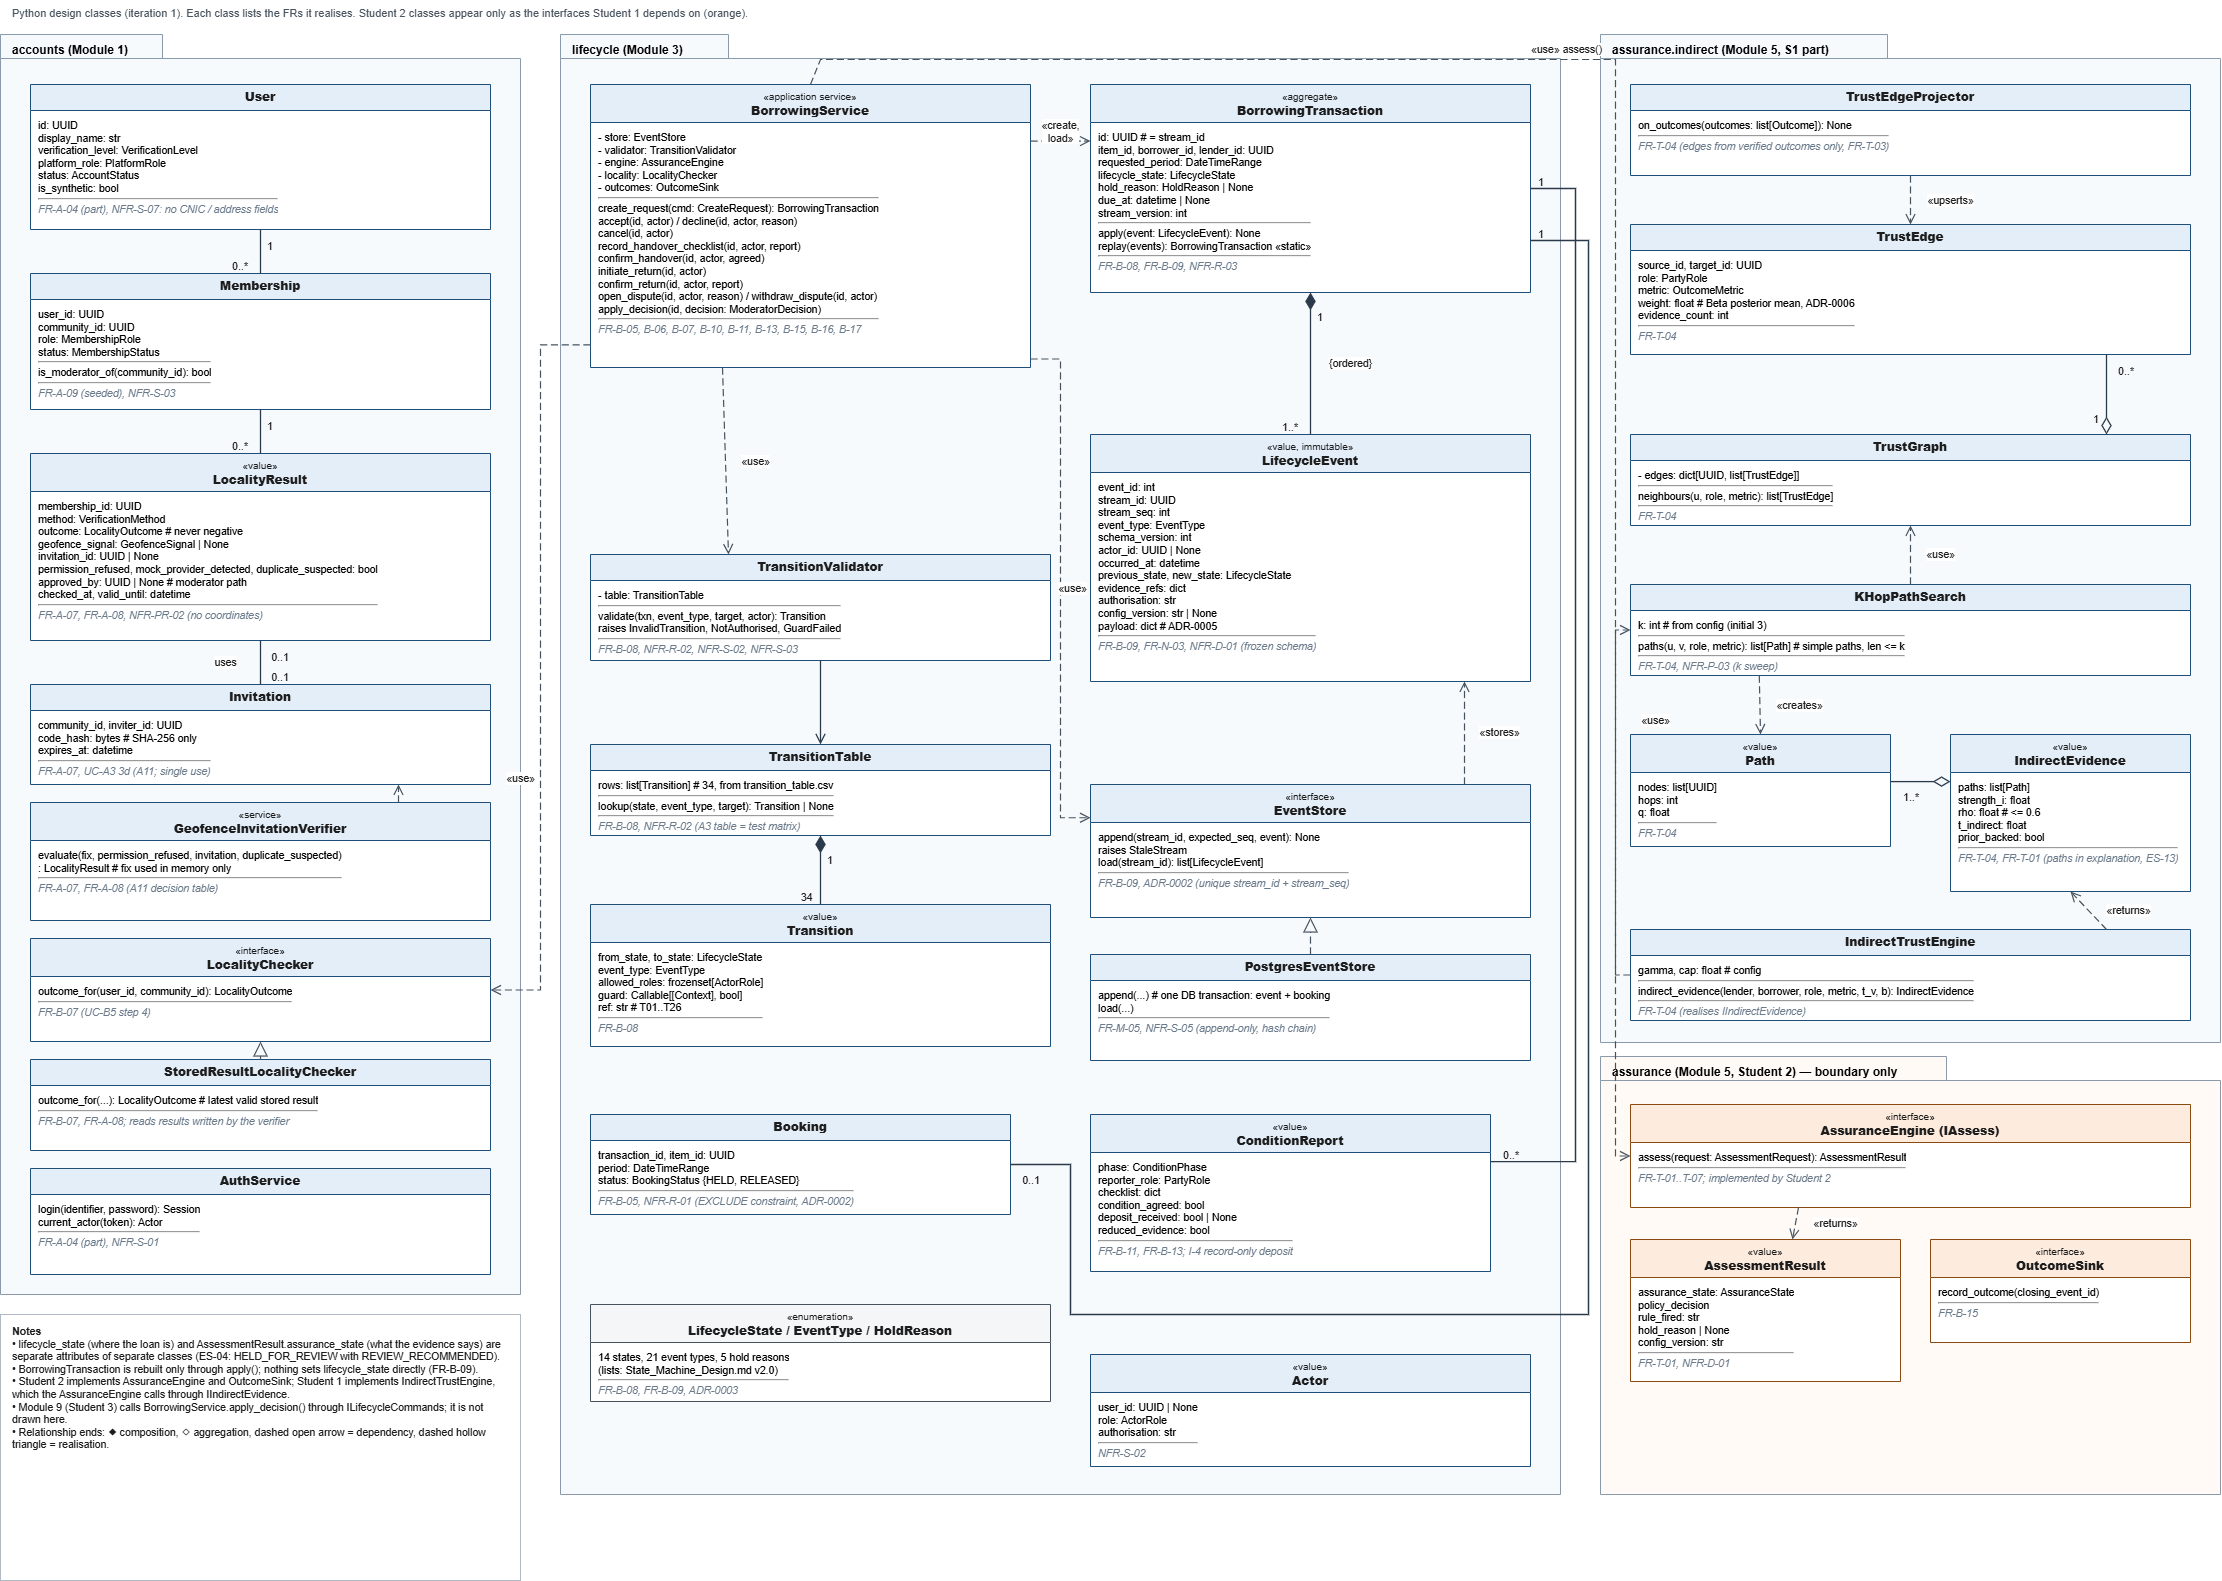
\includegraphics[width=\textheight]{figures/class_s1.png}
\caption{Class diagram, Student 1 packages: accounts and locality, lifecycle and event store, indirect trust}\label{fig:class1}
\end{sidewaysfigure}
\paragraph{Reasoning.} The lifecycle aggregate depends only on the transition table and the ports, so it can be tested without a database; the PostgreSQL event store implements the port. Indirect trust exposes one operation to Student~2's engine. \emph{Serves:} FR-B-05, B-08, B-09, FR-T-04.

\begin{sidewaysfigure}
\centering
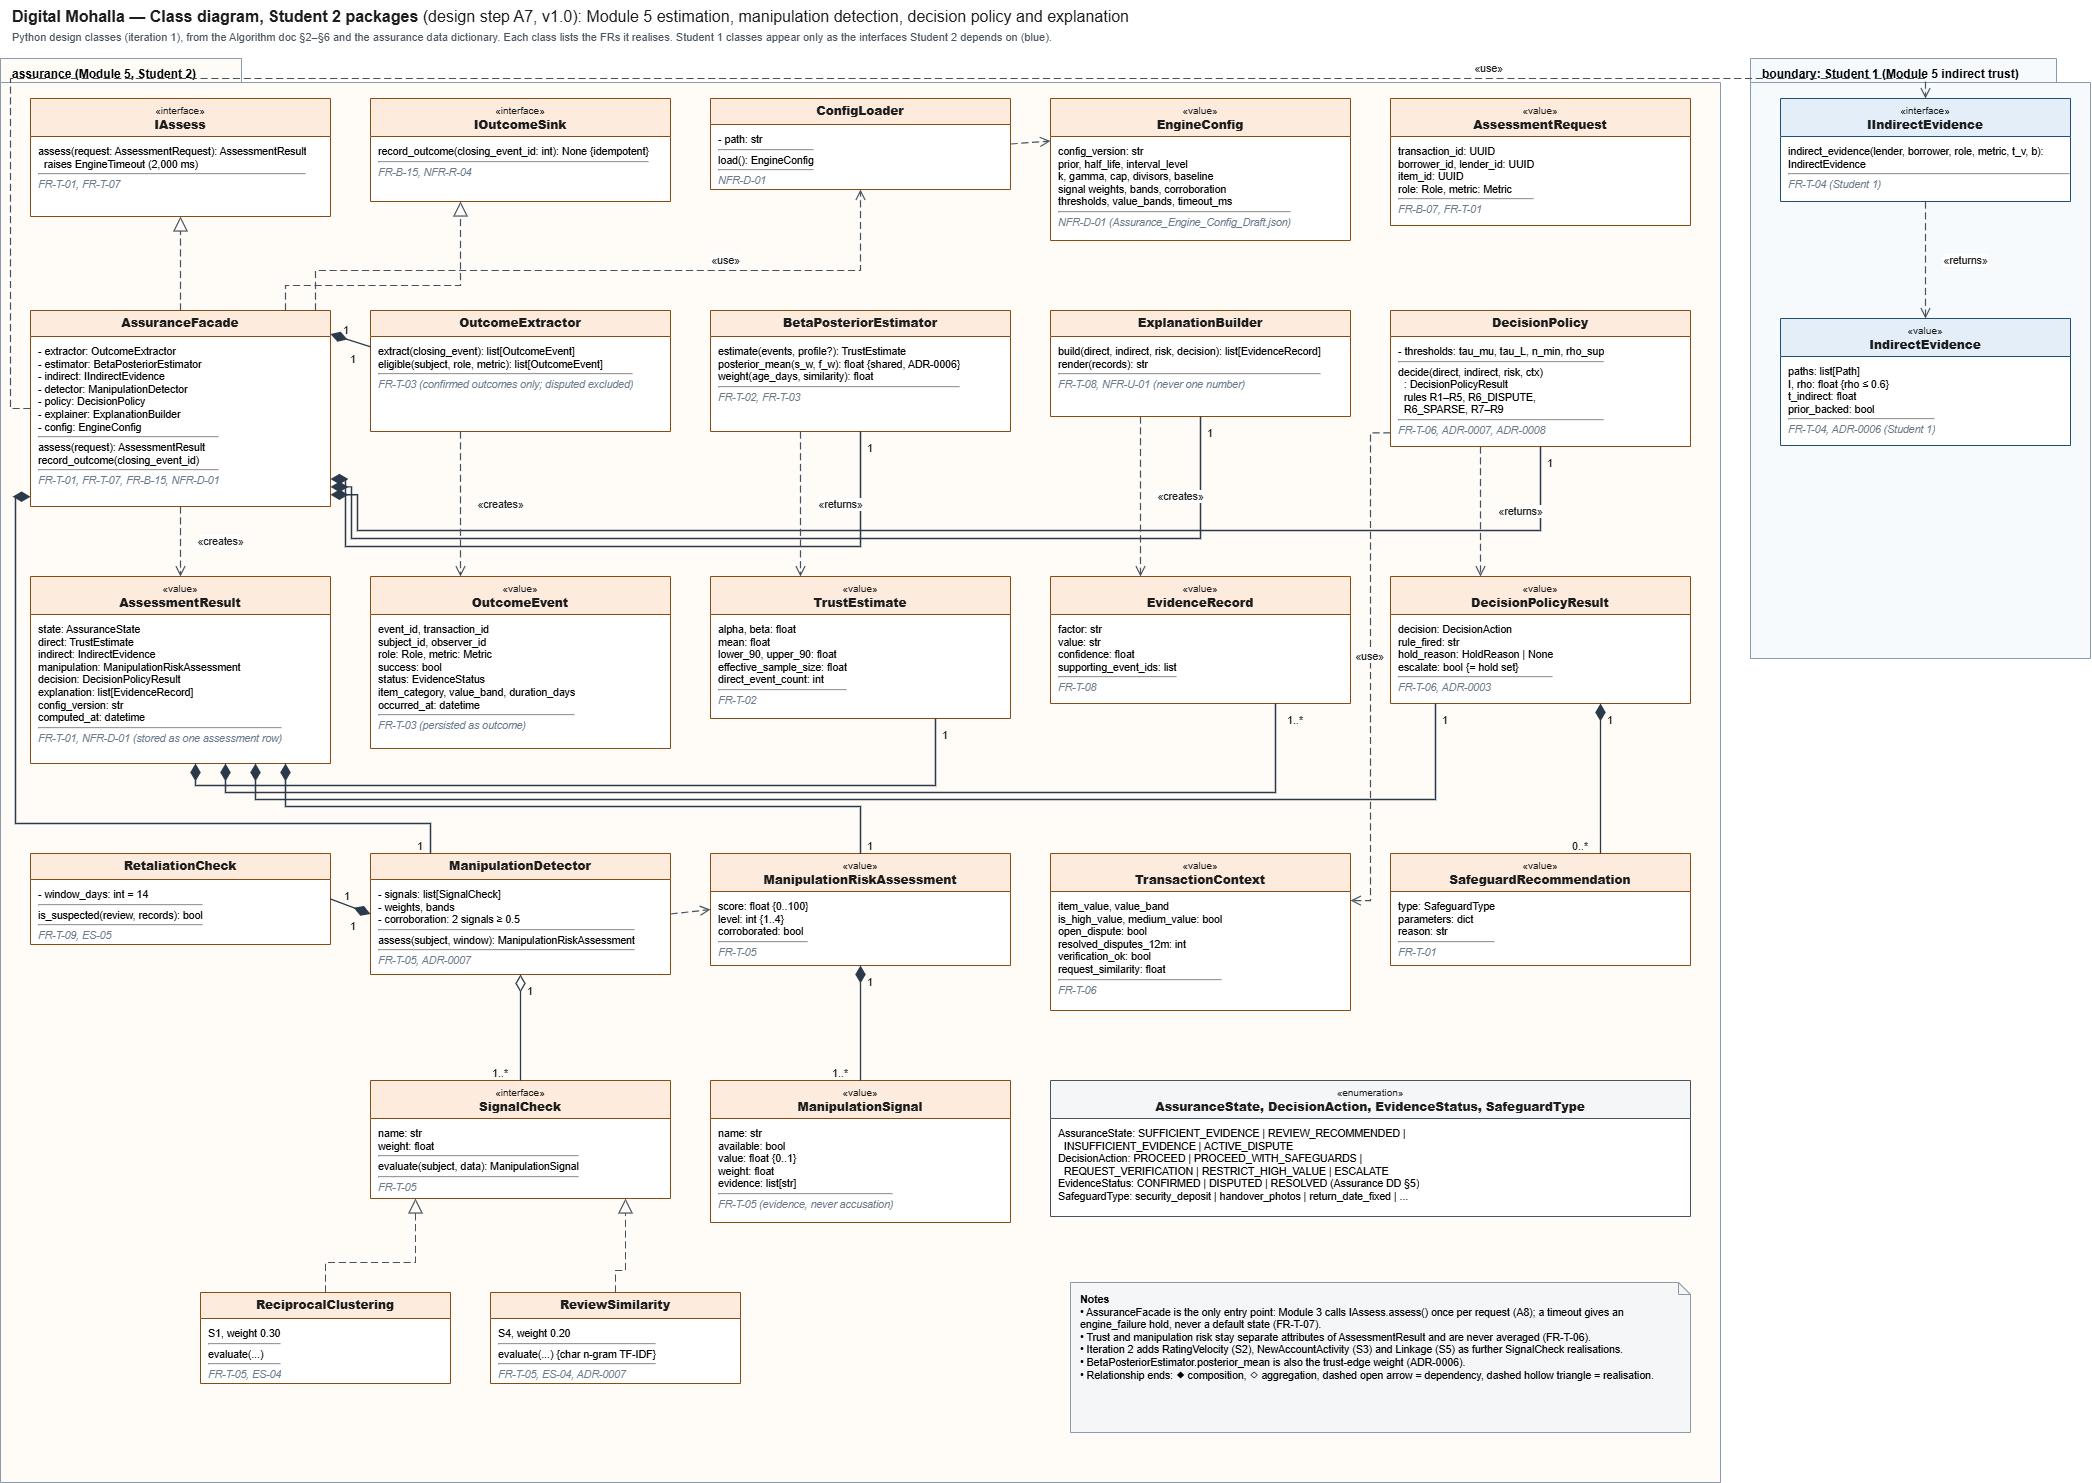
\includegraphics[width=\textheight]{figures/class_s2.png}
\caption{Class diagram, Student 2 packages: estimation, manipulation detection, decision policy and explanation}\label{fig:class2}
\end{sidewaysfigure}
\paragraph{Reasoning.} A single facade runs the pipeline and returns one result object in which trust and manipulation risk are separate attributes, never averaged. Signal checks share one interface so that the Iteration~2 signals (S2, S3, S5) are added without changing the detector. The class named \code{ReciprocalClustering} realises S1, which decision D18 redefined as partner clustering. \emph{Serves:} FR-T-01 to T-08.

\begin{sidewaysfigure}
\centering
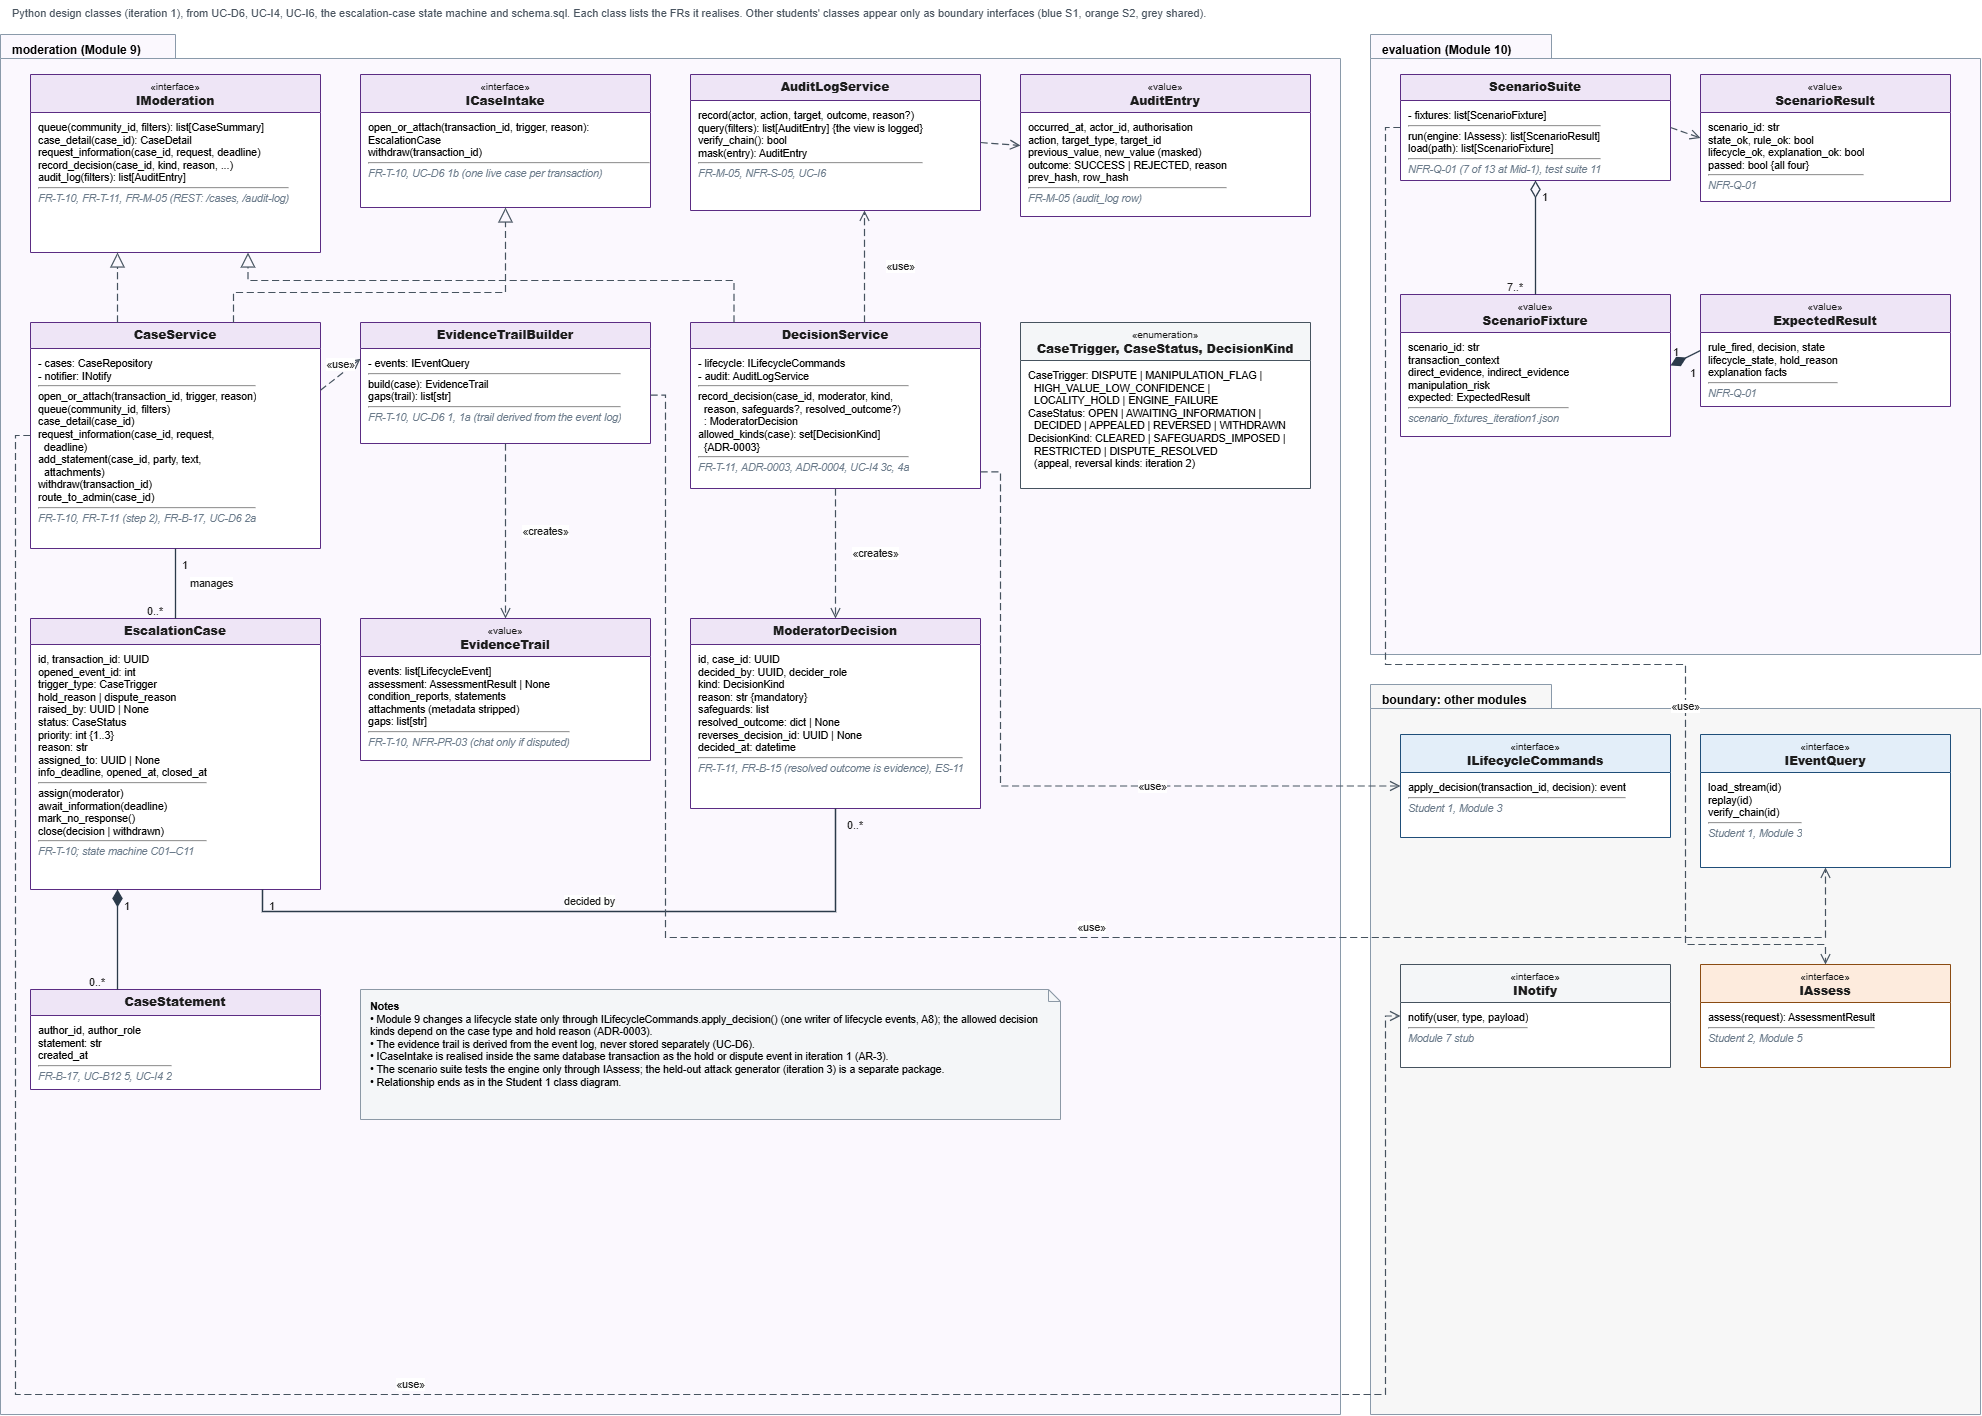
\includegraphics[width=\textheight]{figures/class_s3.png}
\caption{Class diagram, Student 3 packages: cases, decisions and audit (Module 9) and the scenario suite (Module 10)}\label{fig:class3}
\end{sidewaysfigure}
\paragraph{Reasoning.} A moderator decision is a value that the case service turns into exactly one lifecycle command, so moderation cannot bypass the transition rules. \emph{Serves:} FR-T-10, FR-T-11, FR-M-05.

\section{Sequence (b): handover and return to evidence}
\begin{sidewaysfigure}
\centering
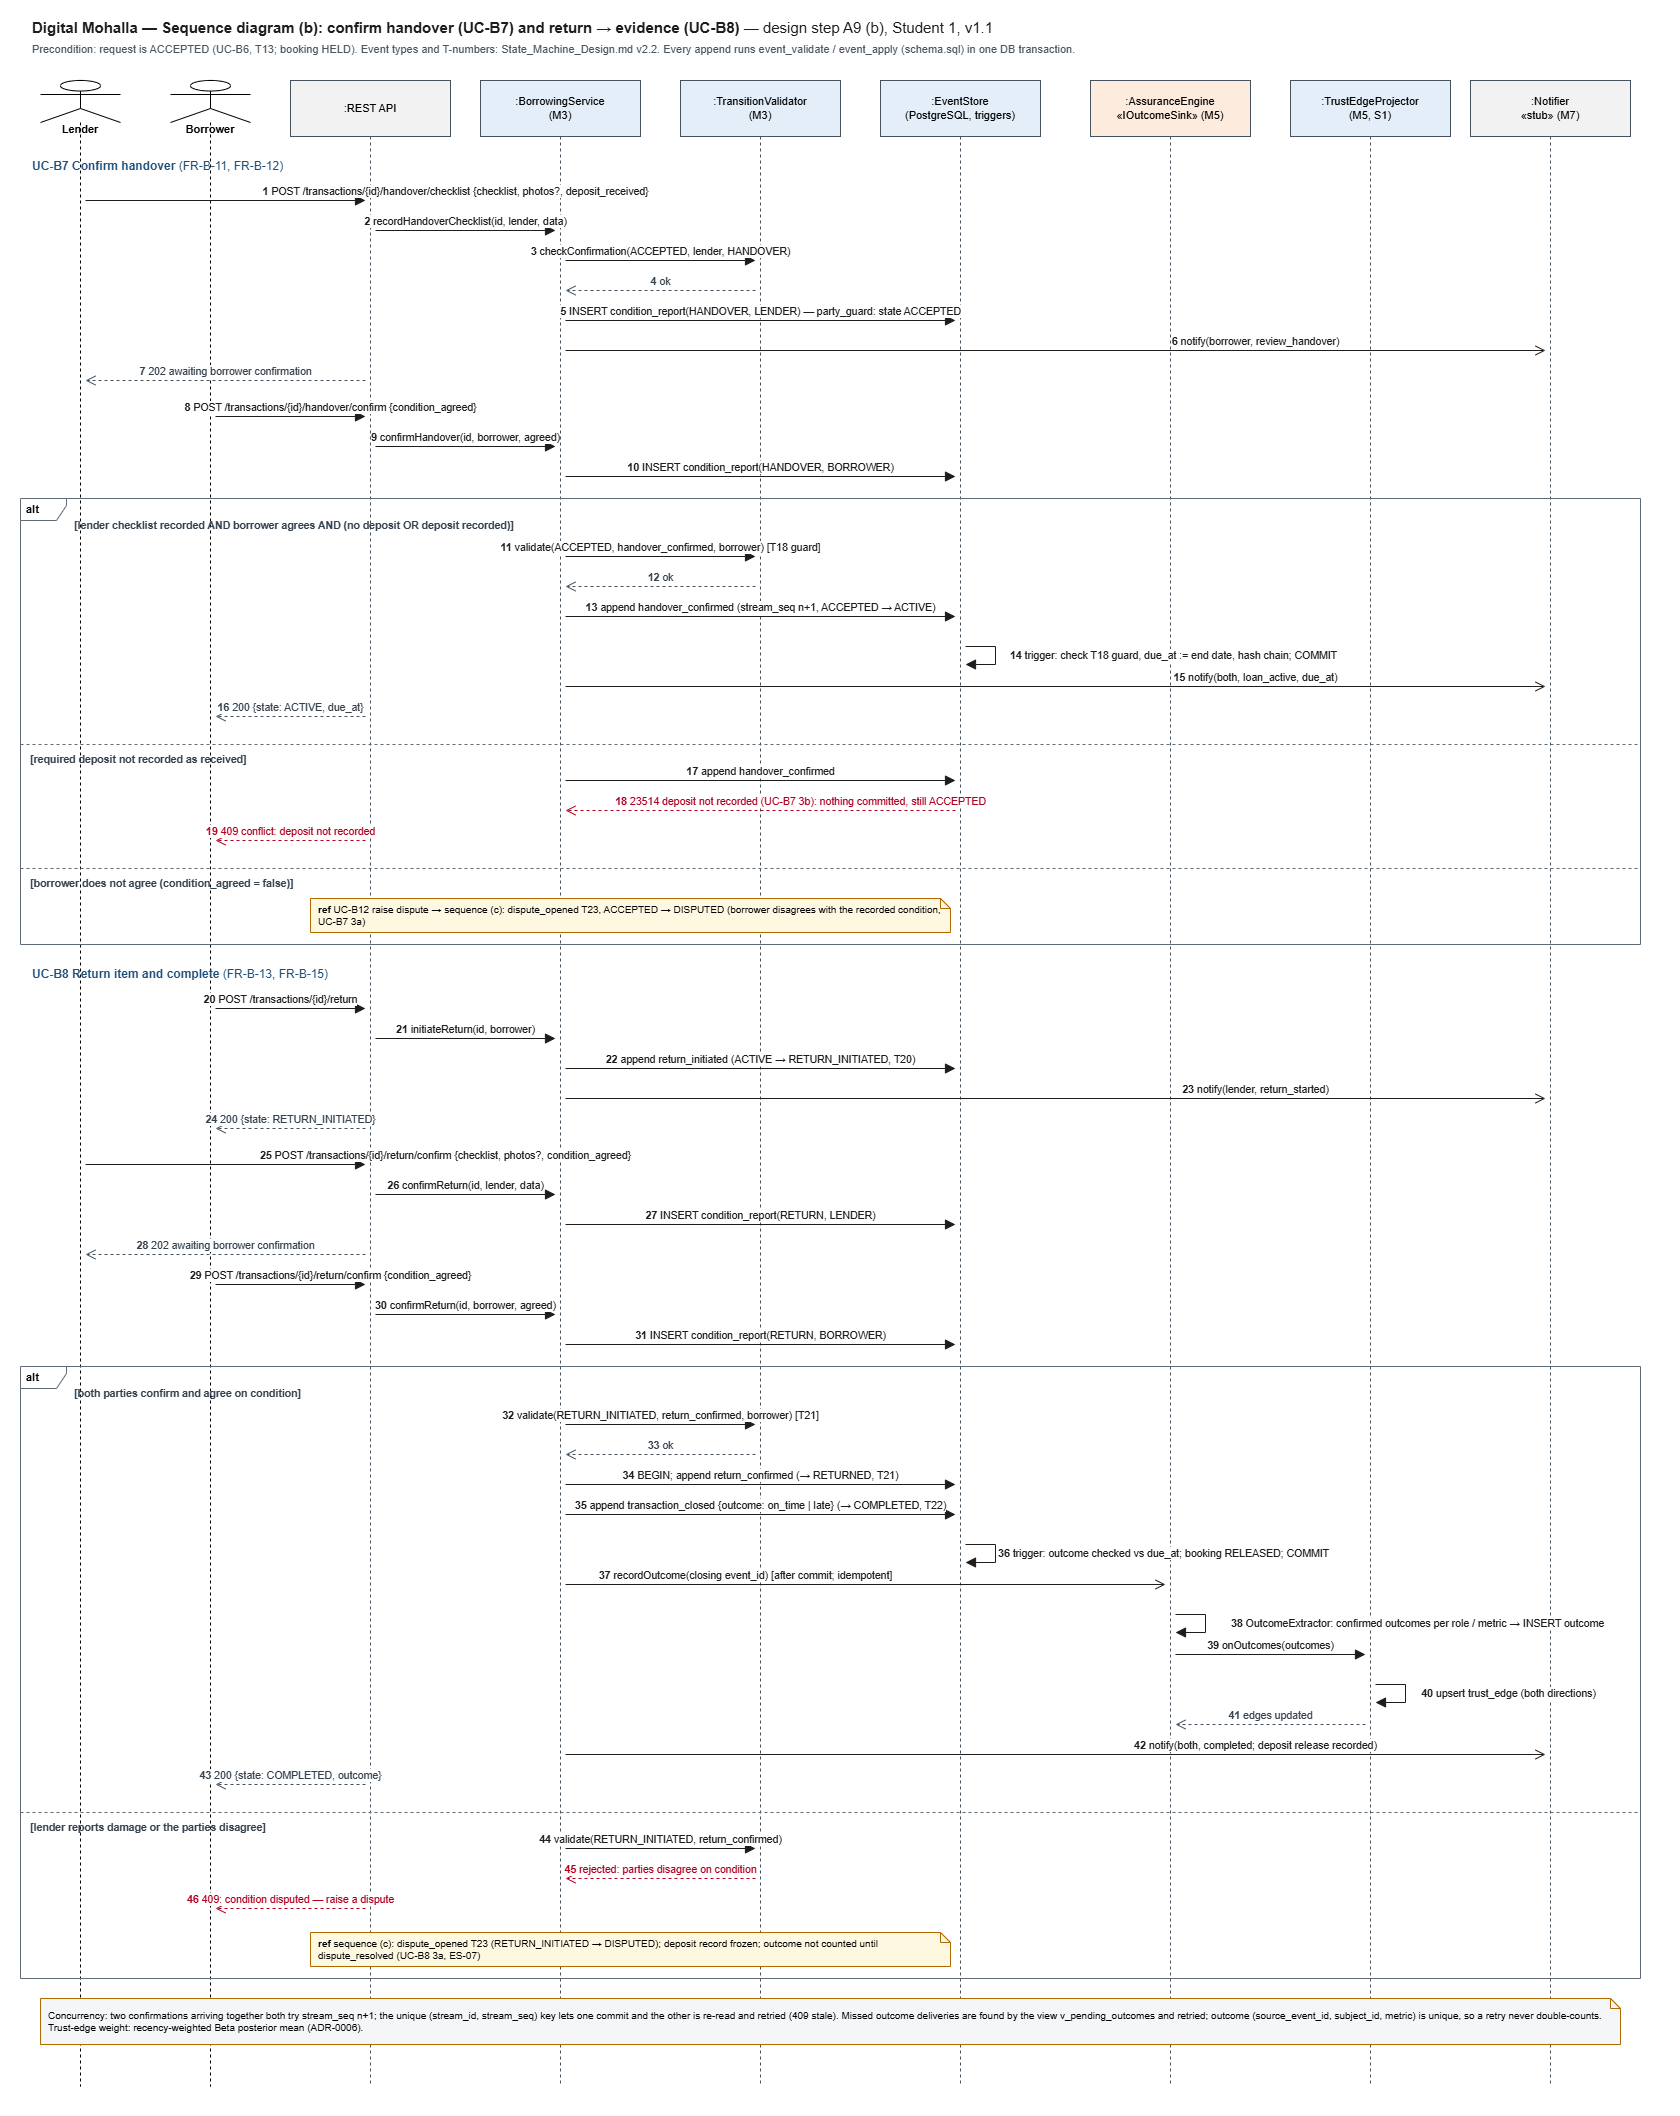
\includegraphics[width=\textheight]{figures/seq_b.png}
\caption{Sequence (b): dual confirmation of handover and return, then outcome to the engine (UC-B7, B8)}\label{fig:seqb}
\end{sidewaysfigure}
\paragraph{Reasoning.} An outcome is written only after both parties have confirmed, which is what makes it ``verified'' evidence (FR-T-03); the close hook writes the outcomes and refreshes the affected trust edges in the same database transaction as \code{transaction\_closed}. \emph{Owner:} S1.

\section{Wireframes}
The wireframes (design step A12, S3) were drawn from the HCI analysis; every screen that shows an assurance state shows its evidence (NFR-U-01). The built screens follow them.

\begin{figure}[H]
\centering
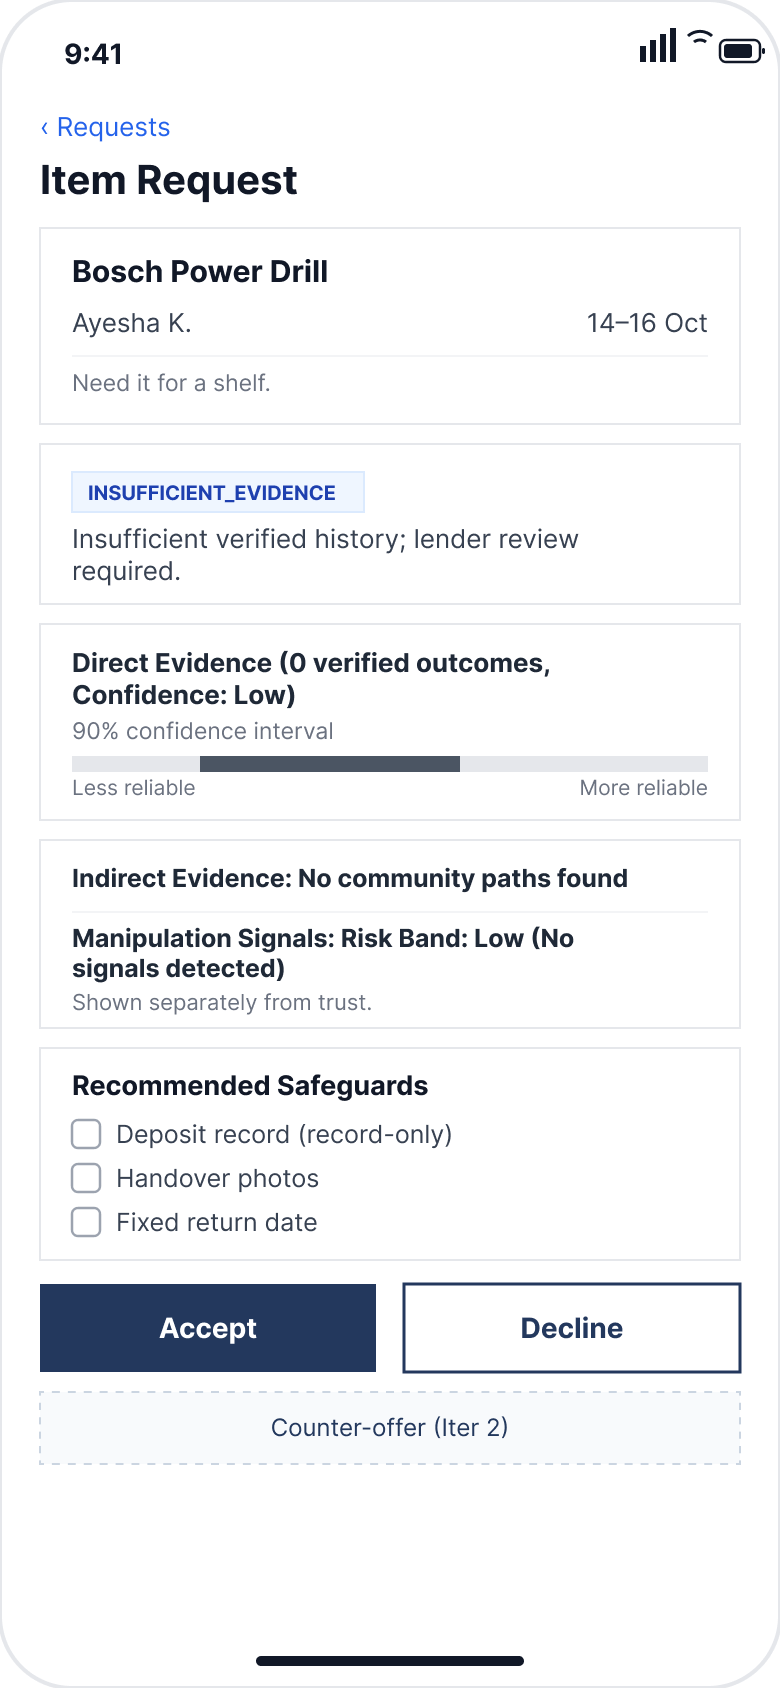
\includegraphics[width=0.45\textwidth]{figures/wf_W1_Lender_Request_Assurance.png}\hfill
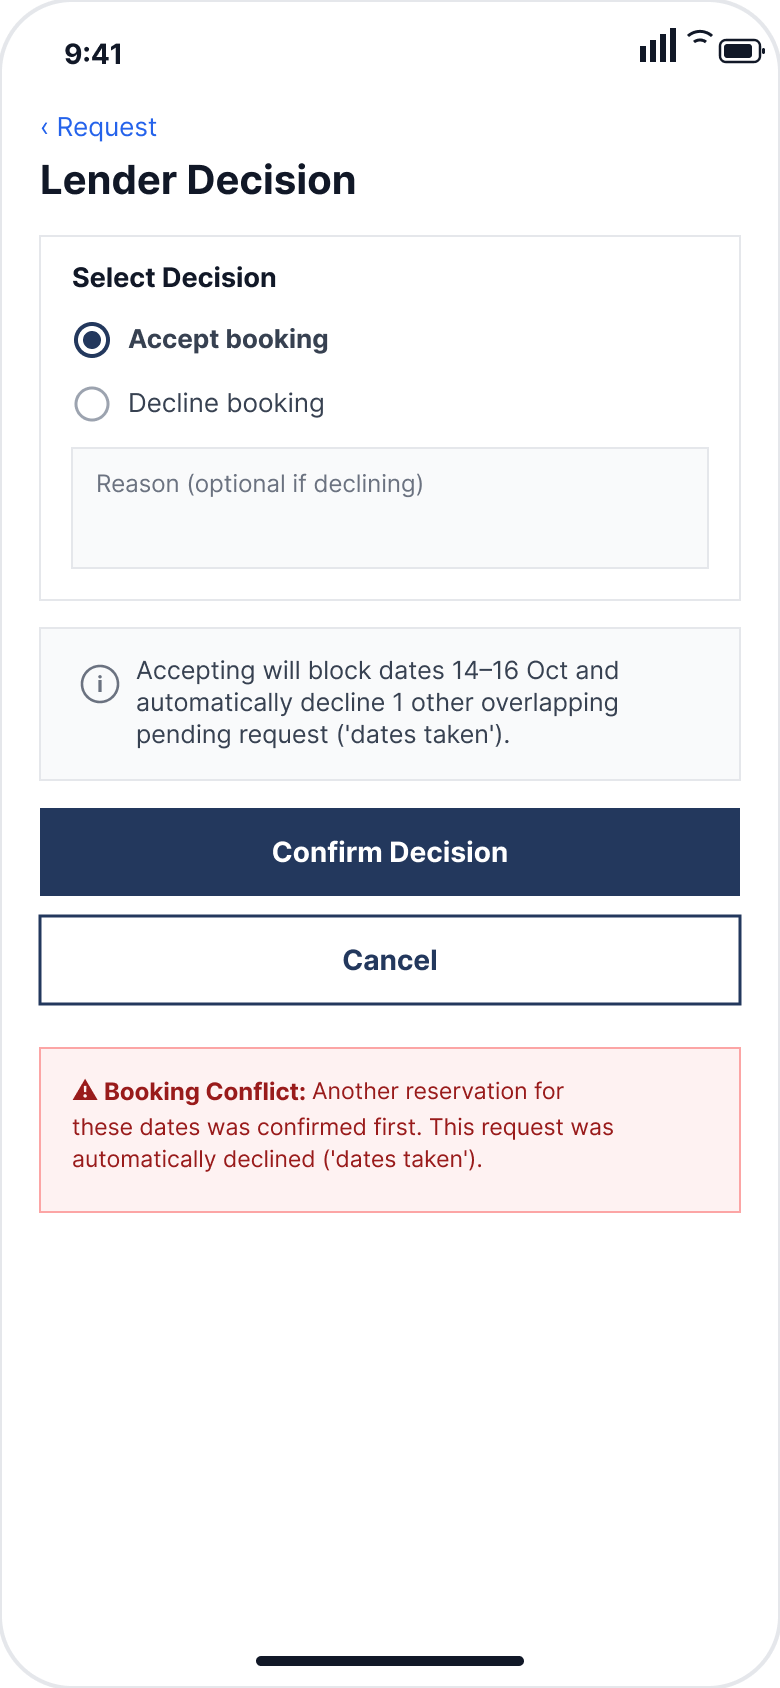
\includegraphics[width=0.45\textwidth]{figures/wf_W2_Lender_Decision_Conflict.png}
\caption{W1 lender request with assurance summary; W2 lender decision and date conflict}\label{fig:w12}
\end{figure}
\begin{figure}[H]
\centering
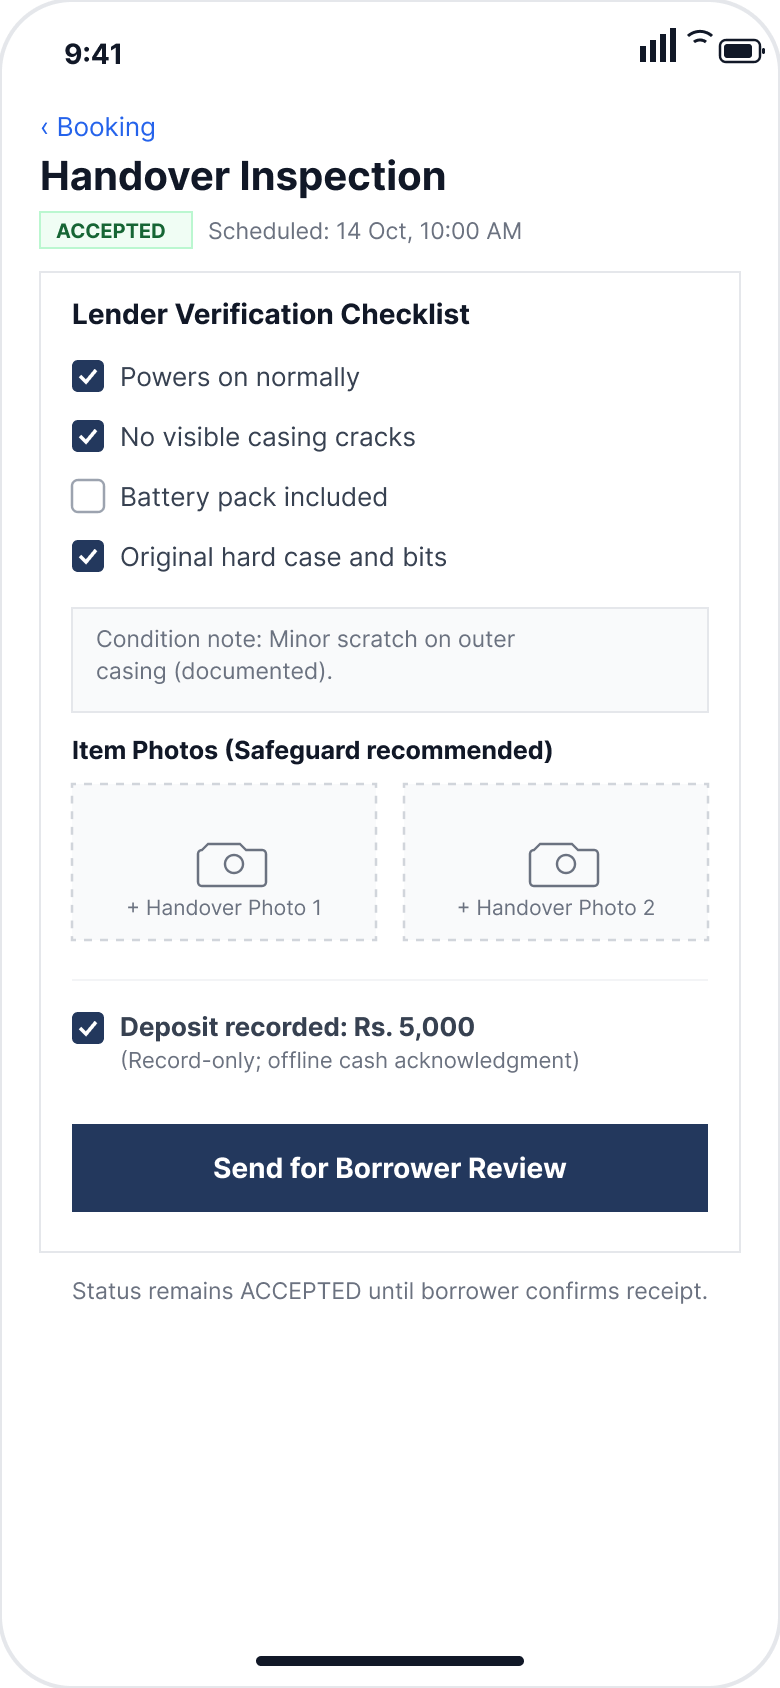
\includegraphics[width=0.45\textwidth]{figures/wf_W3a_Handover_Inspection_Lender.png}\hfill
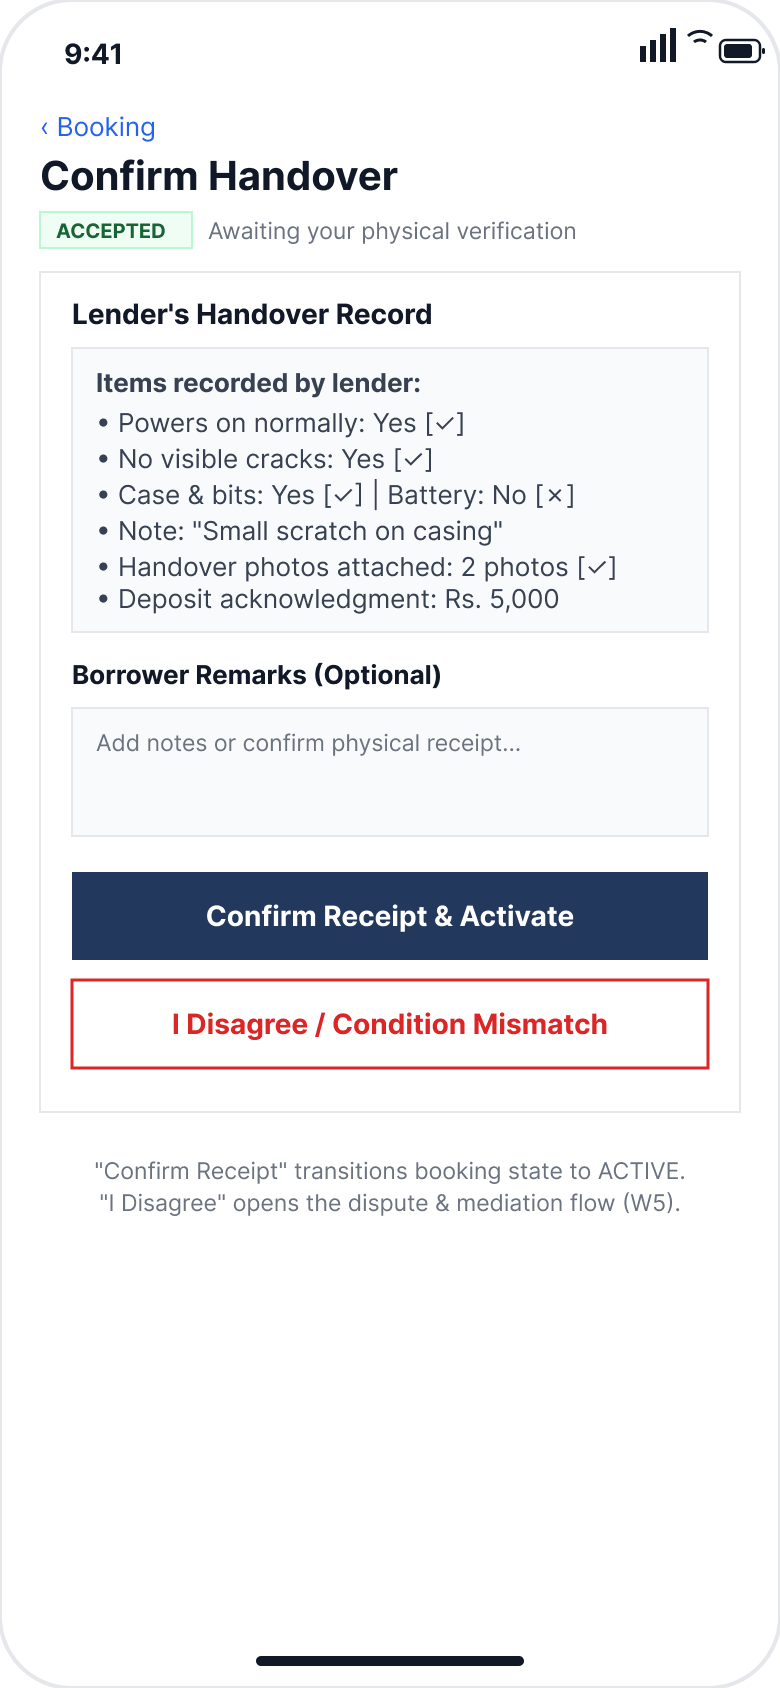
\includegraphics[width=0.45\textwidth]{figures/wf_W3b_Handover_Confirmation_Borrower.png}
\caption{W3a handover inspection (lender); W3b handover confirmation (borrower)}\label{fig:w3}
\end{figure}
\begin{figure}[H]
\centering
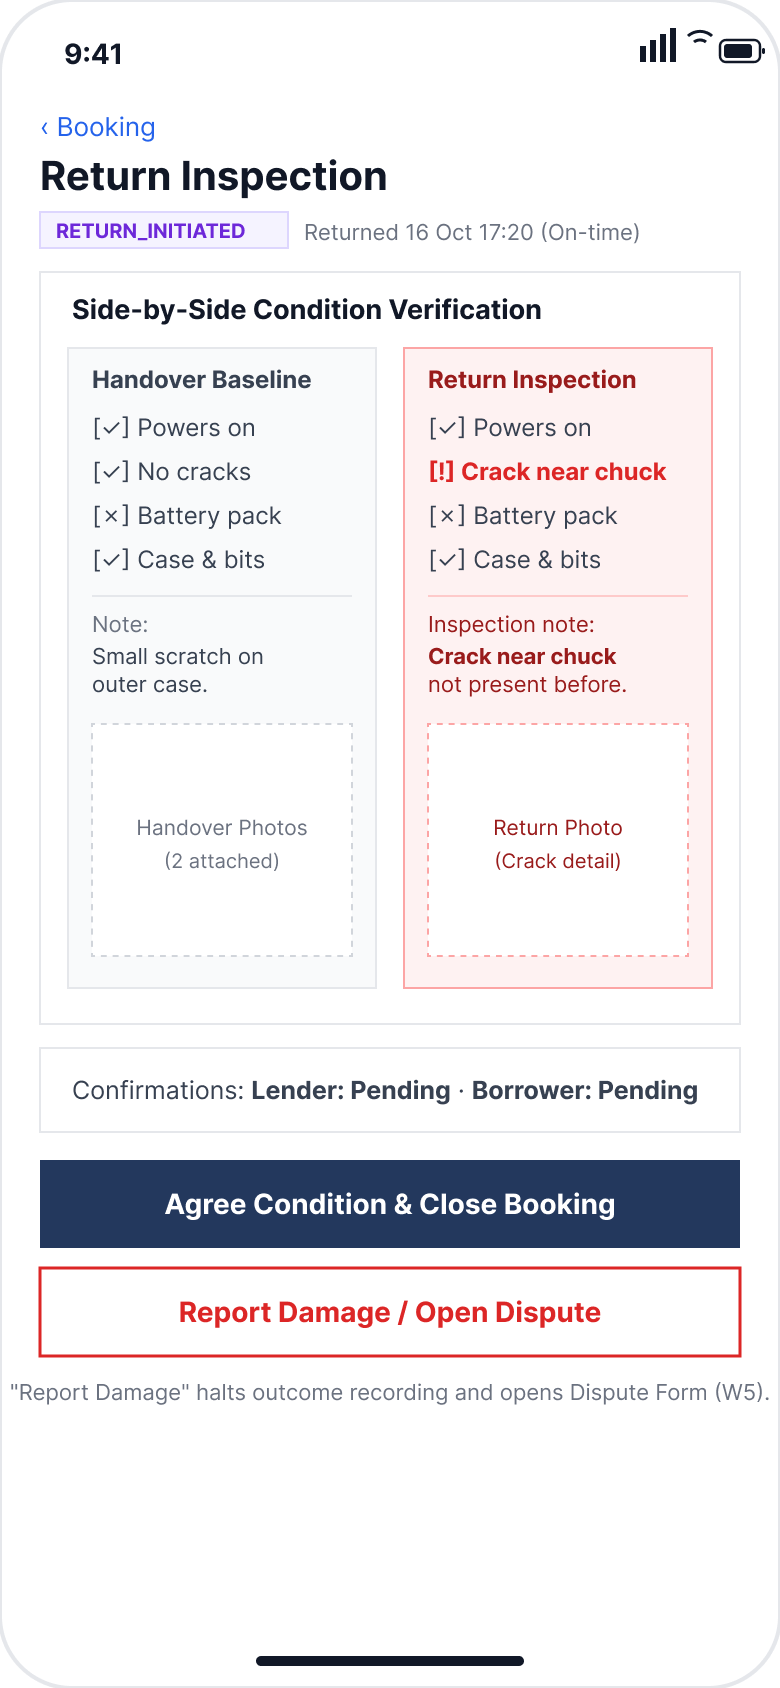
\includegraphics[width=0.45\textwidth]{figures/wf_W4_Return_Inspection_Comparison.png}\hfill
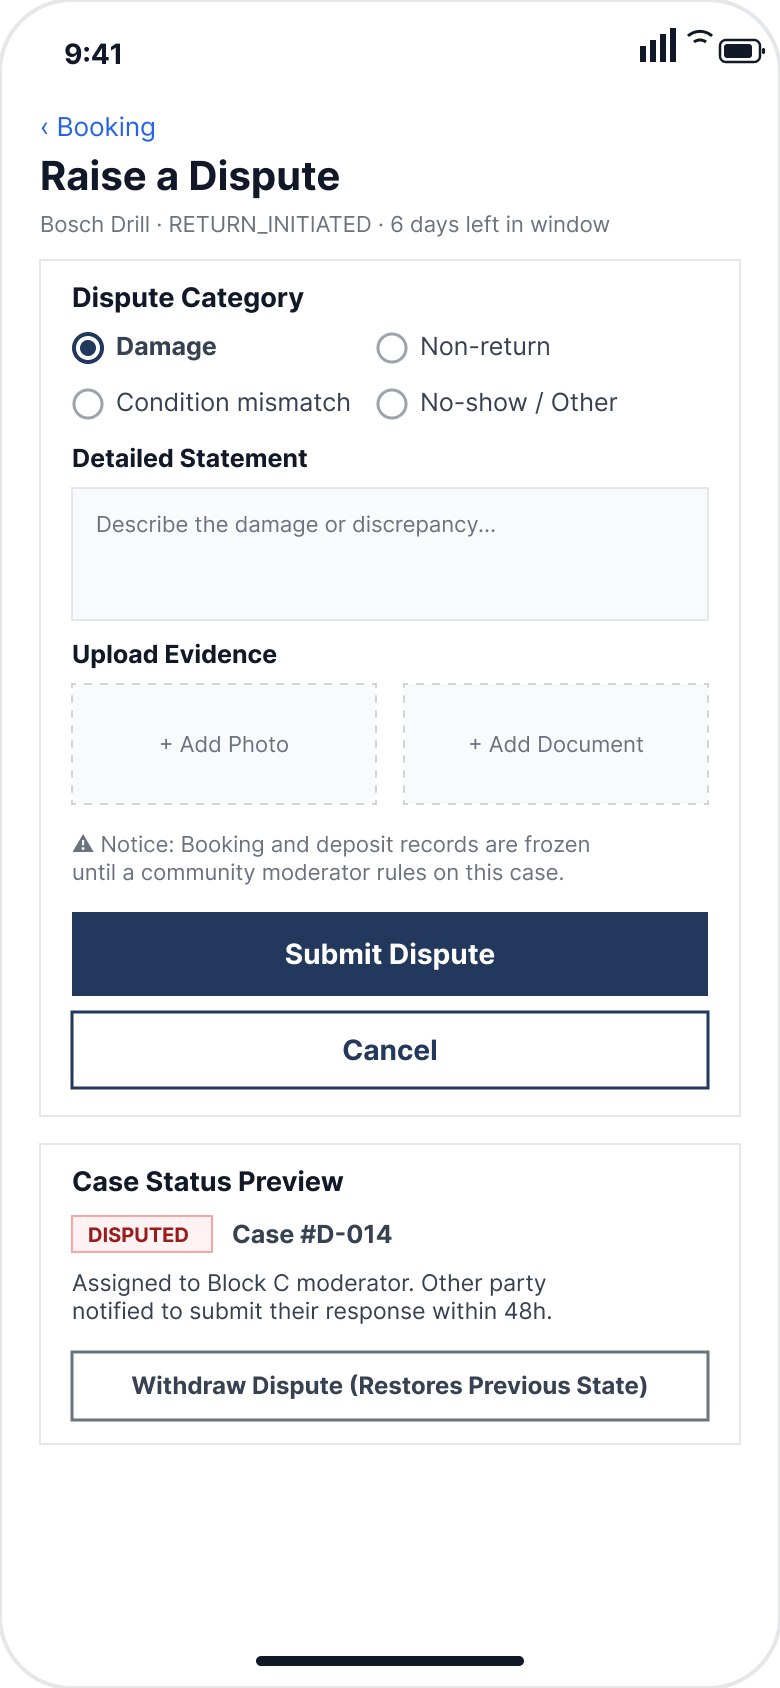
\includegraphics[width=0.45\textwidth]{figures/wf_W5_Dispute_Form_Progress.png}
\caption{W4 return inspection; W5 dispute form and progress}\label{fig:w45}
\end{figure}
\begin{figure}[H]
\centering
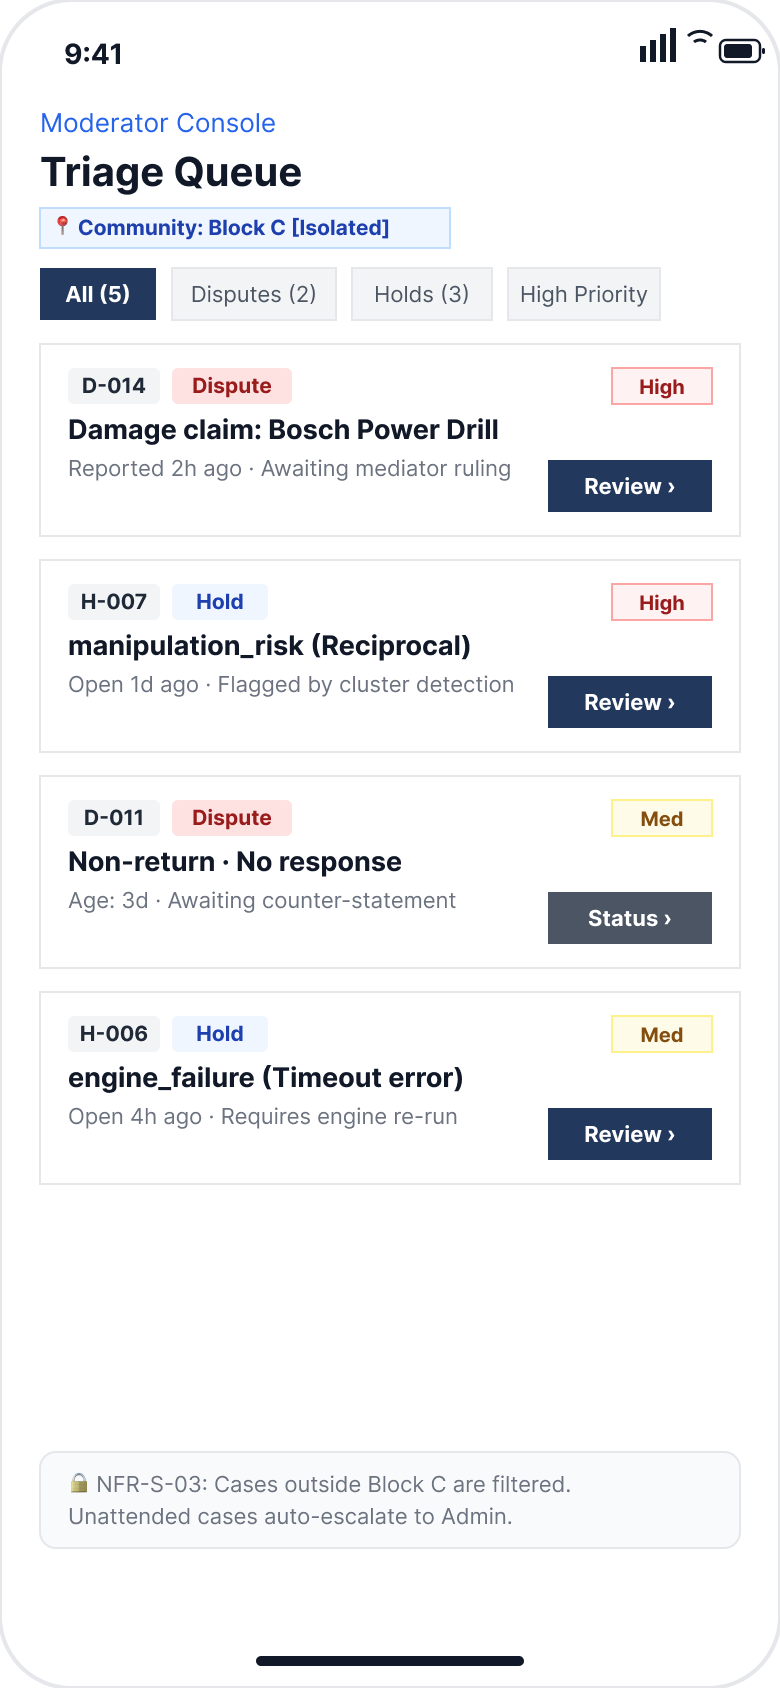
\includegraphics[width=0.45\textwidth]{figures/wf_W6_Moderator_Queue_Mobile.png}\hfill
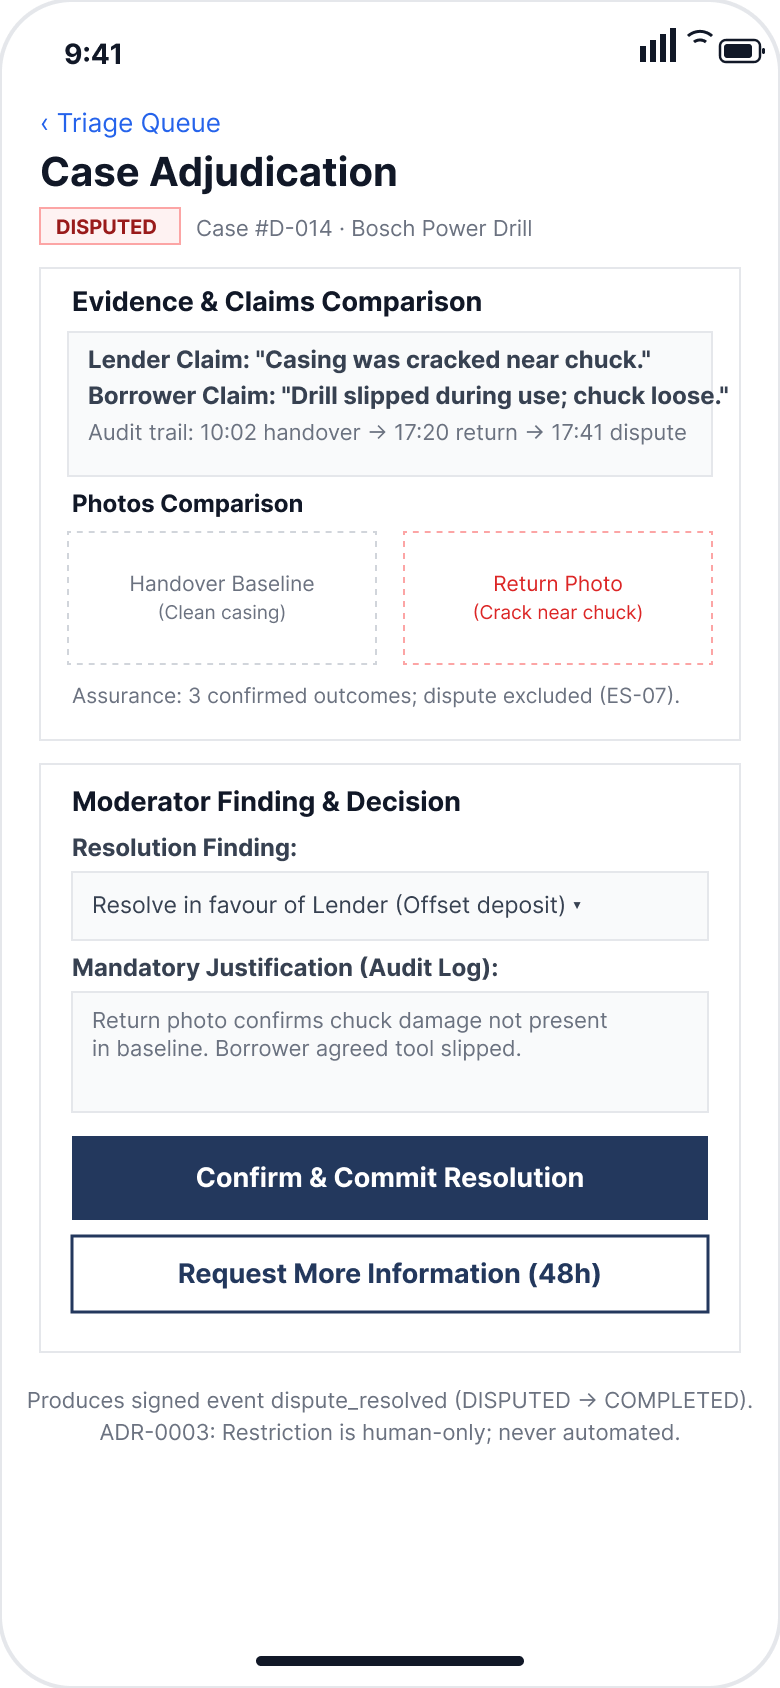
\includegraphics[width=0.45\textwidth]{figures/wf_W7_Moderator_Case_Adjudication_Mobile.png}
\caption{W6 moderator queue; W7 case adjudication}\label{fig:w67}
\end{figure}

\chapter{Meeting and Progress Evidence}\label{app:meeting-progress-evidence}
Team meetings that produced decisions are recorded in \code{docs/design/00_management/}.

\begingroup
\begin{longtable}{@{}L{64pt}L{124pt}L{187pt}@{}}
\caption{Recorded team meetings and reviews}\label{tab:recorded-team-meetings-reviews}\\
\toprule
Date & Record & Outcome \\
\midrule
\endfirsthead
\toprule
Date & Record & Outcome \\
\midrule
\endhead
\bottomrule
\endlastfoot
11 Oct 2026 & Team decisions (design steps A1, A4) & D1--D9: \code{payload} field (ADR-0005); internal event types named; ADR-0001 to 0004 accepted; no disputes from RETURNED; ``RESUME'' dropped; booking hold wording; Request table merged; cancellation from any pending state; case state WITHDRAWN \\
11 Oct 2026 & Integration decisions & The three members' Part A artefacts made one baseline: ADR-0007 and ADR-0008, one vocabulary, engine configuration 1.1.0, privacy boundary at membership, provisional deployment, folder structure \\
11 Oct 2026 & Design review A14 & Every diagram checked against its notation standard; seven faults found and fixed; class diagrams S2 and S3 added \\
13 Oct 2026 & Team decisions (Slice B kickoff) & D10--D16 at kickoff; D17 decided by S2 during B2: edge weight, outcome mapping, thresholds, ES-05 and ES-13 expectations, device scope, test plan use, similarity \\
13--14 Oct 2026 & Team decisions (Slice C) & D18--D20: partner clustering, retaliation handling, upload deferral; confirmed 14 October \\
\end{longtable}
\endgroup


\bibliographystyle{IEEEtran}
\bibliography{references/references}
\end{document}
